\documentclass{solutionclass} % I wrote the design using a4paper, 11pt, twoside, but feel free to change in solutionclass.cls file (line 4)

\pagestyle{plain}

\lstdefinestyle{mystyle}{
	backgroundcolor=\color{backcolour},
	commentstyle=\color{codegreen},
	keywordstyle=\color{magenta},
	numberstyle=\tiny\color{codegray},
	stringstyle=\color{codepurple},
	basicstyle=\ttfamily\normalsize,
	breakatwhitespace=false,
	breaklines=true,
	captionpos=b,
	keepspaces=true,
	numbers=left,
	numbersep=5pt,
	showspaces=false,
	showstringspaces=false,
	showtabs=false,
	tabsize=2
}

\lstset{ %
	language=Python,       % the language of the code
	basicstyle=\footnotesize,       % the size of the fonts that are used for the code
	numbers=left,                   % where to put the line-numbers
	numberstyle=\tiny\color{gray},  % the style that is used for the line-numbers
	stepnumber=1,                   % the step between two line-numbers. If it's 1, each line
	% will be numbered
	numbersep=5pt,                  % how far the line-numbers are from the code
	backgroundcolor=\color{white},  % choose the background color. You must add \usepackage{color}
	showspaces=false,               % show spaces adding particular underscores
	showstringspaces=false,         % underline spaces within strings
	showtabs=false,                 % show tabs within strings adding particular underscores
	frame=single,                   % adds a frame around the code
	rulecolor=\color{black},        % if not set, the frame-color may be changed on line-breaks within not-black text (e.g. commens (green here))
	tabsize=4,                      % sets default tabsize to 2 spaces
	breaklines=true,                % sets automatic line breaking
	breakatwhitespace=false,        % sets if automatic breaks should only happen at whitespace
	% also try caption instead of title
	keywordstyle=\color{blue}, 
    emph=[1]{for,if, end,break},emphstyle=[1]\color{red},         % keyword style
	commentstyle=\color{dkgreen},       % comment style
	stringstyle=\color{mauve},         % string literal style
	escapeinside={\%*}{*)},            % if you want to add a comment within your code
	morekeywords={*,...}               % if you want to add more keywords to the set
}

\hypersetup{
	colorlinks   = true, %Colours links instead of ugly boxes
	urlcolor     = blue, %Colour for external hyperlinks
	linkcolor    = blue, %Colour of internal links
	citecolor   = red %Colour of citations
}

\definecolor{codegreen}{rgb}{0,0.6,0}
\definecolor{codegray}{rgb}{0.5,0.5,0.5}
\definecolor{codepurple}{rgb}{0.58,0,0.82}
\definecolor{backcolour}{rgb}{0.95,0.95,0.92}
\definecolor{mGreen}{rgb}{0,0.6,0}
\definecolor{mGray}{rgb}{0.5,0.5,0.5}
\definecolor{mPurple}{rgb}{0.58,0,0.82}
\definecolor{backgroundColour}{rgb}{0.95,0.95,0.92}

\NewDocumentCommand{\codeword}{v}{
	\texttt{\textcolor{blue}{#1}}
}

\definecolor{dkgreen}{rgb}{0,0.6,0}
\definecolor{gray}{rgb}{0.5,0.5,0.5}
\definecolor{mauve}{rgb}{0.58,0,0.82}

\def\m#1{\boldsymbol{#1}}
\def\co#1{\texttt{#1}}


\begin{document}

\pretitle
{HomeWork 3} % ⟸ Write your main Title here
{Ilia Hashemi Rad}
{99102456}
{AmirMohammad Fakhimi}
{99170531}
{AmirMahdi Namjoo}
{402211467}

% Change your homework number here
\def\homeworkNumber{2}

\makeatletter
    \startcontents[sections]
    \phantomsection
\makeatother
    \def\Solu{Explanations}

\section{Introduction}

\begin{solution}
    In this project, we have implemented a classification problem on sentiment analysis both on a document and text level on the Taaghche comments dataset. Taaghche is an Iranian online ebook marketplace featuring user comments on each book. Based on a dataset of scores and comments from users and other users' likes in the comments, we implemented a classifier for sentiment analysis of the text. We use both base models like LSTM or SVM and also Transfomer-based models.

    In addition, we also wrote a crawler Taaghche website to crawl all the book pages and get the book information like name and author names so that we can have a list of NER for them.
\end{solution}


\section{Crawlers}

\begin{solution}
In the first part, we implemented a crawler on the Taaghche website to get all the book info. The crawler downloads the pages of all books on the website by iterating on the "id" in the URL and saving the result as HTML. We then feed the results into an extractor module written using BeautifulSoup to extract the main parts of book info, including name, publication, author, translator, etc., and save them into CSV files for further use.
\end{solution}

\subsection*{\co{crawler.py}}
\begin{lstlisting}[language=Python]
base_url = "https://taaghche.com/book/"
def save_page(book_id, thread_exceptions):
	url = f"{base_url}{book_id}/"
	try:
		response = requests.get(url)
		
		if response.status_code == 404:
			print(book_id," : 404")
			return
		
		with open(os.path.join(output_dir, f"{book_id}.html"), 'w', encoding='utf-8') as f:
			print(f'Saving book with id: {book_id}')
			f.write(response.text)
	except Exception as e:
		print(e)
		thread_exceptions.append(book_id)

    \end{lstlisting}
\begin{solution}
    This is the main part of the crawler that sends requests to Taagche to get the book pages and save them into files. We also used Python threading features to make the whole process faster.

\end{solution}

\subsection*{\co{extactor.py}}
\begin{lstlisting}[language=Python]
    def extract_data_from_html(file_path):
    with open(file_path, 'r', encoding='utf-8') as file:
        soup = BeautifulSoup(file, 'html.parser')
        script_tag = soup.find('script', type='application/ld+json')
        if script_tag:
            try:
                json_data = json.loads(script_tag.string)
                book_name = json_data.get('name', '')
                authors = ' $ '.join([author['name'] for author in json_data.get('author', [])])
                translators = ' $ '.join(
                    [translator['name'] for translator in json_data.get('workExample', {}).get('translator', [])])
                publisher = json_data.get('workExample', {}).get('publisher', {}).get('name', '')
                data.append({
                    'name': book_name,
                    'author': authors,
                    'translator': translators,
                    'publisher': publisher
                })
            except json.JSONDecodeError:
                pass

    for x in os.listdir(input_dir):
    file_name = x
    file_path = os.path.join(input_dir, file_name)
    if os.path.isfile(file_path) and file_path.endswith('.html'):
        extract_data_from_html(file_path)
    if len(data) >= 10000:
        df = pd.DataFrame(data)
        output_file = os.path.join(output_dir, f'books_data_part_{part_number}.csv')
        df.to_csv(output_file, index=False, encoding='utf-8')
        data = []
        part_number += 1
        print("index put into files: ", file_name)

if data:
    df = pd.DataFrame(data)
    output_file = os.path.join(output_dir, f'books_data_part_{part_number}.csv')
    df.to_csv(output_file, index=False, encoding='utf-8')
    data = []
    part_number += 1
    print("index put into files: ", file_name)
    data = []
\end{lstlisting}

\begin{solution}
The main part of extracor.py is \co{extract\_data\_from\_html} function. This function uses BS4 to find the JSON section that includes book data in the HTML and save data json data into a python dictionary. This data is then fed into a Pandas Dataframe and we save it into a csv file.


\end{solution}

\section{Document Classifier -  Base Model}

The base model is in \co{DocClassifier\_Base.ipynb}. We investigate each segment in the following sections.



Note: Some parts of the explanations of code from here to the end of the document are written by partially ChatGPT to help us write clear and unambiguous descriptions.


\subsection*{Loading and Preparing Data}


\begin{lstlisting}[language=Python]
# Import the pandas library for data manipulation
import pandas as pd

# Load the CSV file into a pandas DataFrame
# The file 'taghche.csv' is located in the 'datasets/' directory
data = pd.read_csv('datasets/taghche.csv')

# Remove any duplicate rows in the DataFrame
data = data.drop_duplicates()

# Drop rows where the 'comment' or 'rate' columns have missing values (NaN)
data.dropna(subset=['comment', 'rate'], inplace=True)

# Print the first 5 rows of the cleaned DataFrame
print(data.head())


def label_sentiment(rate, positive_threshold, neutral_threshold):
"""
Labels sentiment based on rating thresholds.

Args:
- rate (int or float): The numerical rating to evaluate.
- positive_threshold (int or float): The minimum rating value that qualifies as 'positive'.
- neutral_threshold (int or float): The minimum rating value that qualifies as 'neutral'; ratings below this are considered 'negative'.

Returns:
- str: The sentiment label ('positive', 'neutral', or 'negative') based on the rating.
"""
# Check if the rating is greater than or equal to the positive threshold
if rate >= positive_threshold:
return 'positive'
# If the rating is not 'positive', check if it is greater than or equal to the neutral threshold
elif rate >= neutral_threshold:
return 'neutral'
# If the rating is neither 'positive' nor 'neutral', label the sentiment as 'negative'
else:
return 'negative'
\end{lstlisting}

\begin{solution}
At first, we load data using Pandas Library. We then define a fucntion to label the sentiment of each comment based on its rating and threshold. note that we have two thresholds, one for positive, and one for neutral comments. everything below neutral is considered negative.
\end{solution}



\subsection*{Balancing Data}


\begin{lstlisting}[language=Python]
	# Function to prepare data and labels based on given thresholds
def prepare_data(positive_threshold, neutral_threshold):
    """
    Prepares the data and labels based on given thresholds for sentiment classification.

    Args:
    - positive_threshold (int or float): The minimum rating value that qualifies as 'positive'.
    - neutral_threshold (int or float): The minimum rating value that qualifies as 'neutral'; ratings below this are considered 'negative'.

    Returns:
    - tuple: A tuple containing:
        - pandas.Series: The comments from the balanced dataset.
        - pandas.Series: The corresponding sentiment labels from the balanced dataset.
    """
    # Create a copy of the original data to avoid modifying it
    labeled_data = data.copy()
    
    # Apply the label_sentiment function to the 'rate' column to create a new 'sentiment' column
    labeled_data['sentiment'] = labeled_data['rate'].apply(lambda x: label_sentiment(x, positive_threshold, neutral_threshold))
    
    # Combine the 'comment' and 'sentiment' columns into a single DataFrame
    df = pd.concat([labeled_data['comment'], labeled_data['sentiment']], axis=1)

    # Separate the DataFrame into three classes based on sentiment
    positive = df[df['sentiment'] == 'positive']
    neutral = df[df['sentiment'] == 'neutral']
    negative = df[df['sentiment'] == 'negative']

    # Determine the size of the smallest class to balance the dataset
    min_class_size = min(len(positive), len(neutral), len(negative))

    # Downsample each class to the size of the smallest class to ensure balance
    positive_downsampled = resample(positive, replace=False, n_samples=min_class_size, random_state=42)
    neutral_downsampled = resample(neutral, replace=False, n_samples=min_class_size, random_state=42)
    negative_downsampled = resample(negative, replace=False, n_samples=min_class_size, random_state=42)

    # Combine the downsampled classes into a single DataFrame
    df_balanced = pd.concat([positive_downsampled, neutral_downsampled, negative_downsampled])

    # Shuffle the balanced DataFrame to mix the rows
    df_balanced = df_balanced.sample(frac=1, random_state=42).reset_index(drop=True)
    
    # Return the 'comment' and 'sentiment' columns as separate pandas Series
    return df_balanced['comment'], df_balanced['sentiment']
\end{lstlisting}

\begin{solution}
\begin{itemize}
	\item The function starts by creating a copy of the original dataset to avoid modifying it:
	\begin{lstlisting}[language=Python]
		labeled_data = data.copy()
	\end{lstlisting}
	
	\item It applies the \texttt{label\_sentiment} function to the \texttt{rate} column to create a new \texttt{sentiment} column:
	\begin{lstlisting}[language=Python]
		labeled_data['sentiment'] = labeled_data['rate'].apply(lambda x: label_sentiment(x, positive_threshold, neutral_threshold))
	\end{lstlisting}
	
	\item The function then combines the \texttt{comment} and \texttt{sentiment} columns into a single DataFrame:
	\begin{lstlisting}[language=Python]
		df = pd.concat([labeled_data['comment'], labeled_data['sentiment']], axis=1)
	\end{lstlisting}
	
	\item It separates the DataFrame into three classes based on sentiment:
	\begin{lstlisting}[language=Python]
		positive = df[df['sentiment'] == 'positive']
		neutral = df[df['sentiment'] == 'neutral']
		negative = df[df['sentiment'] == 'negative']
	\end{lstlisting}
	
	\item The function determines the size of the smallest class to balance the dataset:
	\begin{lstlisting}[language=Python]
		min_class_size = min(len(positive), len(neutral), len(negative))
	\end{lstlisting}
	
	\item It down-samples each class to the size of the smallest class to ensure balance:
	\begin{lstlisting}[language=Python]
		positive_downsampled = resample(positive, replace=False, n_samples=min_class_size, random_state=42)
		neutral_downsampled = resample(neutral, replace=False, n_samples=min_class_size, random_state=42)
		negative_downsampled = resample(negative, replace=False, n_samples=min_class_size, random_state=42)
	\end{lstlisting}
	
	\item The function combines the down-sampled classes into a single DataFrame:
	\begin{lstlisting}[language=Python]
		df_balanced = pd.concat([positive_downsampled, neutral_downsampled, negative_downsampled])
	\end{lstlisting}
	
	\item It shuffles the balanced DataFrame to mix the rows:
	\begin{lstlisting}[language=Python]
		df_balanced = df_balanced.sample(frac=1, random_state=42).reset_index(drop=True)
	\end{lstlisting}
	
	\item Finally, the function returns the \texttt{comment} and \texttt{sentiment} columns as separate pandas Series:
	\begin{lstlisting}[language=Python]
		return df_balanced['comment'], df_balanced['sentiment']
	\end{lstlisting}
\end{itemize}
\end{solution}




\subsection*{Preprocess}


\begin{lstlisting}[language=Python]
	# Function to preprocess and normalize the text
def preprocess(text):
    """
    Preprocesses and normalizes text data by removing special characters,
    non-Persian characters, digits, and multiple spaces.

    Args:
    - text (str): Input text to be processed.

    Returns:
    - str: Processed text with normalized format.
    """
    # Replace one or more newline characters with a single newline
    pattern = re.compile(r"\n+")
    text = pattern.sub("\n", text)
    
    # Replace '\n' and '\n' with a single space
    text = re.sub(r'\\n|\n', ' ', text)
    
    # Remove non-Persian characters and digits
    text = re.sub(r'[^آ-ی\s]', ' ', text)
    
    # Replace one or more spaces with a single space
    pattern = re.compile(r" +")
    text = pattern.sub(" ", text)
    
    return text

# Apply the preprocess function to the 'comment' column in the DataFrame data
data['comment'] = data['comment'].apply(preprocess)
# Remove any duplicate rows in the DataFrame
data = data.drop_duplicates()

# Drop rows where the 'comment' or 'rate' columns have missing values (NaN)
data.dropna(subset=['comment', 'rate'], inplace=True)
\end{lstlisting}

\begin{solution}
	\begin{itemize}
        \item The function starts by replacing one or more newline characters with a single newline:
        \begin{lstlisting}[language=Python]
        pattern = re.compile(r"\n+")
        text = pattern.sub("\n", text)
        \end{lstlisting}
    
        \item Next, it replaces occurrences of the newline character (\verb*|\n|) and escaped newline (\verb*|\\n|) with a single space:
        \begin{lstlisting}[language=Python]
        text = re.sub(r'\\n|\n', ' ', text)
        \end{lstlisting}
    
        \item The function then removes all non-Persian characters and digits. This is done using a regular expression that matches any character not in the Persian alphabet (آ-ی) or whitespace:
        \begin{lstlisting}[language=Python]
        text = re.sub(r'[^آ-ی\s]', ' ', text)
        \end{lstlisting}
    
        \item Finally, it replaces one or more spaces with a single space to normalize the spacing in the text:
        \begin{lstlisting}[language=Python]
        pattern = re.compile(r" +")
        text = pattern.sub(" ", text)
        \end{lstlisting}
    
        \item The processed text is then returned by the function.
    \end{itemize}
    
    The following lines apply the \texttt{preprocess} function to the \texttt{comment} column of the DataFrame \texttt{data}:
    
    \begin{lstlisting}[language=Python]
    # Apply the preprocess function to the 'comment' column in the DataFrame data
    data['comment'] = data['comment'].apply(preprocess)
    
    # Remove any duplicate rows in the DataFrame
    data = data.drop_duplicates()
    
    # Drop rows where the 'comment' or 'rate' columns have missing values (NaN)
    data.dropna(subset=['comment', 'rate'], inplace=True)
    \end{lstlisting}
    
    \begin{itemize}
        \item The \texttt{preprocess} function is applied to each entry in the \texttt{comment} column to clean and normalize the text.
        \item After preprocessing, any duplicate rows in the DataFrame are removed using:
        \begin{lstlisting}[language=Python]
        data = data.drop_duplicates()
        \end{lstlisting}
        \item Finally, rows where the \texttt{comment} or \texttt{rate} columns have missing values (NaN) are dropped:
        \begin{lstlisting}[language=Python]
        data.dropna(subset=['comment', 'rate'], inplace=True)
        \end{lstlisting}
    \end{itemize}
    
\end{solution}




\subsection*{TF IDF - Logistic Regression}

Next, we implement a TF-IDF vectorizer and use logistic regression for the task. Based on our study and the papers we investigated, logistic regression is the best base model for this task.


\begin{lstlisting}[language=Python]
	# Create a pipeline with TF-IDF and logistic regression
logReg_PL = Pipeline([
    ("tfidf", TfidfVectorizer()),
    ("logreg", LogisticRegression(max_iter=500, solver='newton-cg'))
])

# Define the parameter grid for GridSearchCV
param_grid = {
    'tfidf__ngram_range': [(1, 1), (1, 2), (1, 3)],
    'tfidf__max_features': [5000, 10000],
    'logreg__C': [0.01, 0.1, 1, 10]
}

# Custom GridSearchCV implementation to iterate over parameter grid
best_score = 0
best_params = None

# Thresholds to evaluate
rate_thresholds = [(1, 2), (1, 3), (1, 4), (2, 3), (2, 4), (3, 4)]

# Iterate over each pair of thresholds and perform GridSearchCV
for neutral_threshold, positive_threshold in tqdm(rate_thresholds):
    # Prepare the data using the specified thresholds
    X_prepared, y_prepared = prepare_data(positive_threshold, neutral_threshold)
    
    # Split the data into training and testing sets
    X_train, X_test, y_train, y_test = train_test_split(X_prepared, y_prepared, test_size=0.1, random_state=42)
    
    # Initialize GridSearchCV with the pipeline and parameter grid
    grid_search = GridSearchCV(logReg_PL, param_grid, cv=5, scoring='accuracy')
    
    # Fit GridSearchCV on the training data
    grid_search.fit(X_train, y_train)
    
    # Get the best score and parameters from GridSearchCV
    score = grid_search.best_score_
    
    # Update the best score and best parameters if the current score is better
    if score > best_score:
        best_score = score
        best_params = grid_search.best_params_
        best_params['positive_threshold'] = positive_threshold
        best_params['neutral_threshold'] = neutral_threshold

# Print the best parameters found by GridSearchCV
print("Best parameters for TF-IDF model are:", best_params)

# Prepare the data using the best parameters found from GridSearchCV
X_prepared, y_prepared = prepare_data(best_params['positive_threshold'], best_params['neutral_threshold'])

# Split the prepared data into training and testing sets
X_train, X_test, y_train, y_test = train_test_split(X_prepared, y_prepared, test_size=0.1, random_state=42)

# Create a pipeline for the best Logistic Regression model with the best parameters
best_logReg_model = Pipeline([
    ("tfidf", TfidfVectorizer(ngram_range=best_params['tfidf__ngram_range'], max_features=best_params['tfidf__max_features'])),
    ("logreg", LogisticRegression(C=best_params['logreg__C'], max_iter=500, solver='newton-cg'))
])

# Fit the best Logistic Regression model on the training data
best_logReg_model.fit(X_train, y_train)

# Predict the labels on the test set using the best model
y_test_pred = best_logReg_model.predict(X_test)

# Calculate the accuracy score of the best model on the test set
test_accuracy = accuracy_score(y_test, y_test_pred)

# Print the test accuracy score of the best Logistic Regression model
print("Test accuracy of Logistic Regression model:", test_accuracy)
\end{lstlisting}

\begin{solution}
	\begin{lstlisting}[language=Python]
        logReg_PL = Pipeline([
            ("tfidf", TfidfVectorizer()),
            ("logreg", LogisticRegression(max_iter=500, solver='newton-cg'))
        ])
        \end{lstlisting}
        
        \begin{itemize}
            \item The pipeline \texttt{logReg\_PL} is created with two steps:
            \begin{enumerate}
                \item \texttt{TfidfVectorizer()}: Converts text data into TF-IDF features.
                \item \texttt{LogisticRegression()}: Applies logistic regression for classification, with a maximum of 500 iterations and the 'newton-cg' solver.
            \end{enumerate}
        \end{itemize}
        
        \begin{lstlisting}[language=Python]
        # Define the parameter grid for GridSearchCV
        param_grid = {
            'tfidf__ngram_range': [(1, 1), (1, 2), (1, 3)],
            'tfidf__max_features': [5000, 10000],
            'logreg__C': [0.01, 0.1, 1, 10]
        }
        \end{lstlisting}
        
        \begin{itemize}
            \item The \texttt{param\_grid} defines the hyperparameters for GridSearchCV to search over:
            \begin{itemize}
                \item \texttt{tfidf\_\_ngram\_range}: N-gram ranges (unigrams, bigrams, trigrams).
                \item \texttt{tfidf\_\_max\_features}: Maximum number of features (5000 or 10000).
                \item \texttt{logreg\_\_C}: Inverse of regularization strength (0.01, 0.1, 1, 10).
            \end{itemize}
        \end{itemize}
        
        \begin{lstlisting}[language=Python]
        # Custom GridSearchCV implementation to iterate over parameter grid
        best_score = 0
        best_params = None
        
        # Thresholds to evaluate
        rate_thresholds = [(1, 2), (1, 3), (1, 4), (2, 3), (2, 4), (3, 4)]
        \end{lstlisting}
        
        \begin{itemize}
            \item \texttt{best\_score} and \texttt{best\_params} are initialized to store the best score and corresponding parameters.
            \item \texttt{rate\_thresholds} contains pairs of thresholds to evaluate for neutral and positive sentiment classification.
        \end{itemize}
        
        \begin{lstlisting}[language=Python]
        # Iterate over each pair of thresholds and perform GridSearchCV
        for neutral_threshold, positive_threshold in tqdm(rate_thresholds):
            # Prepare the data using the specified thresholds
            X_prepared, y_prepared = prepare_data(positive_threshold, neutral_threshold)
            
            # Split the data into training and testing sets
            X_train, X_test, y_train, y_test = train_test_split(X_prepared, y_prepared, test_size=0.1, random_state=42)
            
            # Initialize GridSearchCV with the pipeline and parameter grid
            grid_search = GridSearchCV(logReg_PL, param_grid, cv=5, scoring='accuracy')
            
            # Fit GridSearchCV on the training data
            grid_search.fit(X_train, y_train)
            
            # Get the best score and parameters from GridSearchCV
            score = grid_search.best_score_
            
            # Update the best score and best parameters if the current score is better
            if score > best_score:
                best_score = score
                best_params = grid_search.best_params_
                best_params['positive_threshold'] = positive_threshold
                best_params['neutral_threshold'] = neutral_threshold
        
        # Print the best parameters found by GridSearchCV
        print("Best parameters for TF-IDF model are:", best_params)
        \end{lstlisting}
        
        \begin{itemize}
            \item The code iterates over each pair of thresholds in \texttt{rate\_thresholds}.
            \item For each pair:
            \begin{enumerate}
                \item \texttt{prepare\_data} is called to prepare the dataset with the current thresholds.
                \item The data is split into training and testing sets using \texttt{train\_test\_split}.
                \item \texttt{GridSearchCV} is initialized with the pipeline and parameter grid, and fitted to the training data.
                \item The best score and parameters are retrieved from the grid search results.
                \item If the current score is better than the best score, update \texttt{best\_score} and \texttt{best\_params}.
            \end{enumerate}
        \end{itemize}
        
        \begin{lstlisting}[language=Python]
        # Prepare the data using the best parameters found from GridSearchCV
        X_prepared, y_prepared = prepare_data(best_params['positive_threshold'], best_params['neutral_threshold'])
        
        # Split the prepared data into training and testing sets
        X_train, X_test, y_train, y_test = train_test_split(X_prepared, y_prepared, test_size=0.1, random_state=42)
        
        # Create a pipeline for the best Logistic Regression model with the best parameters
        best_logReg_model = Pipeline([
            ("tfidf", TfidfVectorizer(ngram_range=best_params['tfidf__ngram_range'], max_features=best_params['tfidf__max_features'])),
            ("logreg", LogisticRegression(C=best_params['logreg__C'], max_iter=500, solver='newton-cg'))
        ])
        
        # Fit the best Logistic Regression model on the training data
        best_logReg_model.fit(X_train, y_train)
        
        # Predict the labels on the test set using the best model
        y_test_pred = best_logReg_model.predict(X_test)
        
        # Calculate the accuracy score of the best model on the test set
        test_accuracy = accuracy_score(y_test, y_test_pred)
        
        # Print the test accuracy score of the best Logistic Regression model
        print("Test accuracy of Logistic Regression model:", test_accuracy)
        \end{lstlisting}
        
        \begin{itemize}
            \item The data is prepared using the best parameters found by GridSearchCV.
            \item The prepared data is split into training and testing sets.
            \item A pipeline is created for the best logistic regression model with the best parameters.
            \item The model is fitted to the training data.
            \item Predictions are made on the test set.
            \item The accuracy of the model is calculated on the test set.
            \item The test accuracy is printed.
        \end{itemize}
        
\end{solution}




\subsection*{Evaluation Metrics}


\begin{lstlisting}[language=Python]
	def evaluate_model(y_true, y_pred, class_names):
    """
    Evaluates the performance of a classification model using various metrics and visualizations.

    Args:
    - y_true (array-like): True labels of the data.
    - y_pred (array-like): Predicted labels of the data.
    - class_names (list): List of class names in the same order as the confusion matrix.

    Returns:
    - pd.DataFrame: DataFrame containing the classification report.
    """
    # Generate and print the classification report
    report = classification_report(y_true, y_pred, target_names=class_names, output_dict=True)
    report_df = pd.DataFrame(report).transpose()
    print("Classification Report:\n", report_df)

    # Generate and display the confusion matrix as a heatmap
    cm = confusion_matrix(y_true, y_pred)
    plt.figure(figsize=(10, 7))
    sns.heatmap(cm, annot=True, fmt='d', cmap='Blues', xticklabels=class_names, yticklabels=class_names)
    plt.xlabel('Predicted')
    plt.ylabel('True')
    plt.title('Confusion Matrix')
    plt.show()

    # Calculate and print overall metrics: accuracy, precision, recall, and F1 score
    accuracy = accuracy_score(y_true, y_pred)
    precision = precision_score(y_true, y_pred, average='weighted')
    recall = recall_score(y_true, y_pred, average='weighted')
    f1 = f1_score(y_true, y_pred, average='weighted')

    metrics = {
        "Accuracy": accuracy,
        "Precision": precision,
        "Recall": recall,
        "F1 Score": f1
    }

    print("\nOverall Metrics:")
    for metric, value in metrics.items():
        print(f"{metric}: {value:.4f}")
    
    return report_df

# Evaluate the model
report_df = evaluate_model(y_test, y_test_pred, ["Negative", "Neutral", "Positive"])
\end{lstlisting}

\begin{solution}
	The \texttt{evaluate\_model} function evaluates the performance of a classification model using various metrics and visualizations.
\begin{itemize}
    \item The function takes three arguments:
    \begin{itemize}
        \item \texttt{y\_true}: The true labels of the data.
        \item \texttt{y\_pred}: The predicted labels of the data.
        \item \texttt{class\_names}: A list of class names in the same order as the confusion matrix.
    \end{itemize}
    \item The function returns a pandas DataFrame containing the classification report.
\end{itemize}

\subsection*{Classification Report}

\begin{itemize}
    \item The classification report is generated using \texttt{classification\_report} from scikit-learn and printed:
    \begin{lstlisting}[language=Python]
    report = classification_report(y_true, y_pred, target_names=class_names, output_dict=True)
    report_df = pd.DataFrame(report).transpose()
    print("Classification Report:\n", report_df)
    \end{lstlisting}
\end{itemize}

\subsection*{Confusion Matrix}

\begin{itemize}
    \item The confusion matrix is generated and displayed as a heatmap using seaborn:
    \begin{lstlisting}[language=Python]
    cm = confusion_matrix(y_true, y_pred)
    plt.figure(figsize=(10, 7))
    sns.heatmap(cm, annot=True, fmt='d', cmap='Blues', xticklabels=class_names, yticklabels=class_names)
    plt.xlabel('Predicted')
    plt.ylabel('True')
    plt.title('Confusion Matrix')
    plt.show()
    \end{lstlisting}
\end{itemize}

\subsection*{Overall Metrics}

\begin{itemize}
    \item The function calculates and prints overall metrics including accuracy, precision, recall, and F1 score:
    \begin{lstlisting}[language=Python]
    accuracy = accuracy_score(y_true, y_pred)
    precision = precision_score(y_true, y_pred, average='weighted')
    recall = recall_score(y_true, y_pred, average='weighted')
    f1 = f1_score(y_true, y_pred, average='weighted')

    metrics = {
        "Accuracy": accuracy,
        "Precision": precision,
        "Recall": recall,
        "F1 Score": f1
    }

    print("\nOverall Metrics:")
    for metric, value in metrics.items():
        print(f"{metric}: {value:.4f}")
    \end{lstlisting}
    \item These metrics are printed in a readable format.
\end{itemize}

\subsection*{Function Return}

\begin{itemize}
    \item The function returns the classification report DataFrame:
    \begin{lstlisting}[language=Python]
    return report_df
    \end{lstlisting}
\end{itemize}

\subsection*{Model Evaluation}

\begin{itemize}
    \item The \texttt{evaluate\_model} function is called to evaluate the model:
    \begin{lstlisting}[language=Python]
    report_df = evaluate_model(y_test, y_test_pred, ["Negative", "Neutral", "Positive"])
    \end{lstlisting}
\end{itemize}
\end{solution}


\subsection{Results and Interesting Notes}

For the results section, we analyzed different approaches to the data to check whether we could get a better result. At first, we tested it without any special technique and got an accuracy of about 0.61 on the whole data. Another approach we tested is removing stopwords, but it seems stopwords are important for our task, and after removing them, our accuracy dropped.


Another approach was to use a formalizer to change the text into a formal Persian text. We used a formalizer based on T5 using models from previous semesters, but we got worse results. It is predictable, though, because some informal Persian slang can significantly change the sentiment of a sentence, and they lose their meaning even from a human perspective when we formalize them.

We also used another approach for formalization: giving the Persian text to Google Translate to translate it into English and then back to Persian. It didn't work fine either.

One of the things we find in papers that seem good for this task is a lemmatizer. We tried to use it on our data, but unfortunately, Hazm was very slow on our 70K database, so we could not use this technique for our task.

It seems our result is good enough, though. As it is a multiclass classification and the best results are for ParsBERT on a significantly larger database than ours that is near 70\%, it seems our accuracy of 61\% is good enough.


The code used for formalization based on T5 is as follows:

\begin{lstlisting}[language=Python]
    from transformers import (T5ForConditionalGeneration, AutoTokenizer, pipeline)
    import torch
    
    model = T5ForConditionalGeneration.from_pretrained('parsi-ai-nlpclass/PersianTextFormalizer')
    tokenizer = AutoTokenizer.from_pretrained('parsi-ai-nlpclass/PersianTextFormalizer')
    
    pipe = pipeline(task='text2text-generation', model=model, tokenizer=tokenizer)
    def formalizer(text):
      device = torch.device('cuda' if torch.cuda.is_available() else 'cpu')  
      model.to(device) 
      formalized = ""
      for line in text.splitlines():
            
          inputs = tokenizer.encode("informal: " + line, return_tensors='pt', max_length=128, truncation=True, padding='max_length')
          inputs = inputs.to(device) 
    
          outputs = model.generate(inputs, max_length=128, num_beams=4)
          formalized = formalized + tokenizer.decode(outputs[0], skip_special_tokens=True) + " "
      return formalized
    
    data['comment'] = data['comment'].apply(formalizer)
\end{lstlisting}



The code used for formalization based on Google Translate is as follows:

\begin{lstlisting}[language=Python]
    import googletrans as gt
    translator = gt.Translator()
    
    def translation(text):
        en_translated = translator.translate(text, 'en', 'fa')
        fa_translated = translator.translate(en_translated.text, 'fa', 'en')
        return fa_translated.text
    
    data['comment'] = data['comment'].apply(translation)
\end{lstlisting}



\begin{figure}[h!]
    \caption{Results of running Logistic Regression on 10000 rows of dataset - With Formalization}
    \centering
    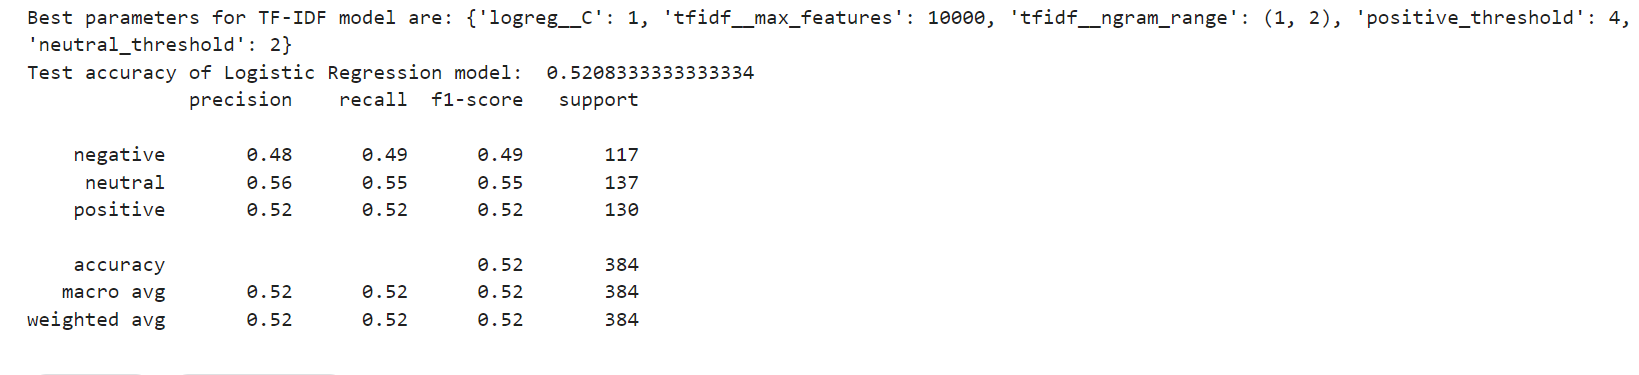
\includegraphics[width=0.5\textwidth]{img/10k_Form.png}
\end{figure}


\begin{figure}[h!]
    \caption{Results of running Logistic Regression on 10000 rows of dataset - Without Formalization}
    \centering
    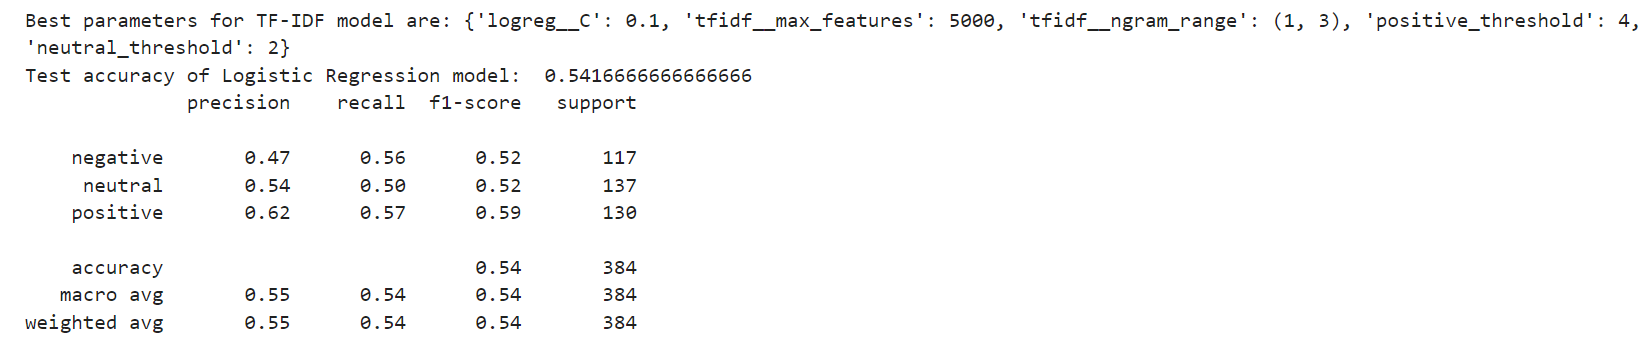
\includegraphics[width=0.5\textwidth]{img/10k_NoForm.png}
\end{figure}



\begin{figure}[h!]
    \caption{Results of running Logistic Regression on 10000 rows of dataset - without stopwords}
    \centering
    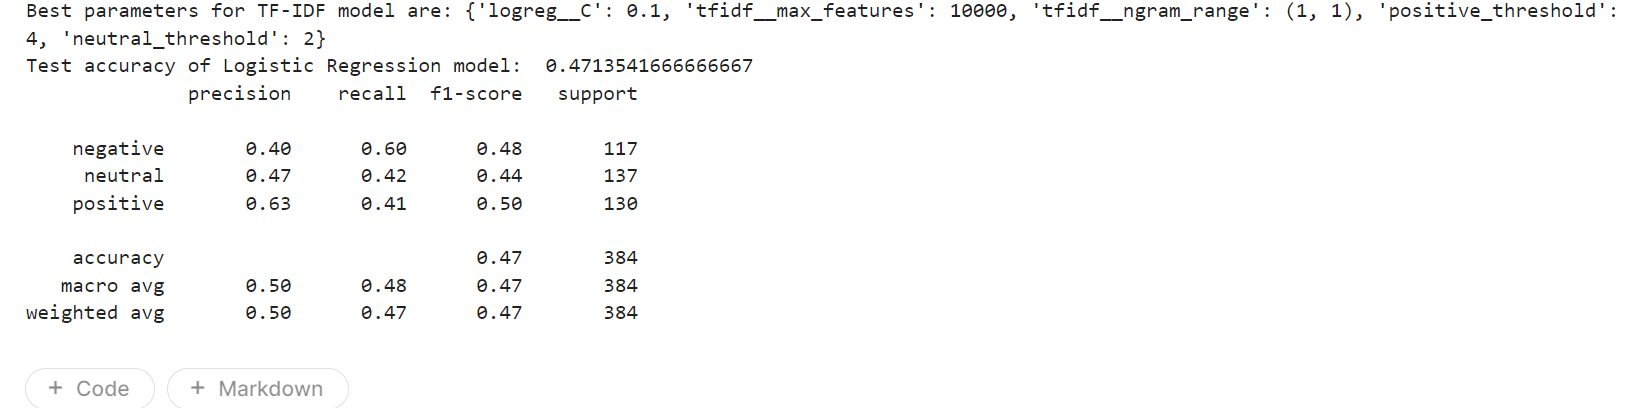
\includegraphics[width=0.5\textwidth]{img/10k_NoSW.png}
\end{figure}


\begin{figure}[h!]
    \caption{Results of running Logistic Regression on 70000 rows of dataset - without stopwords}
    \centering
    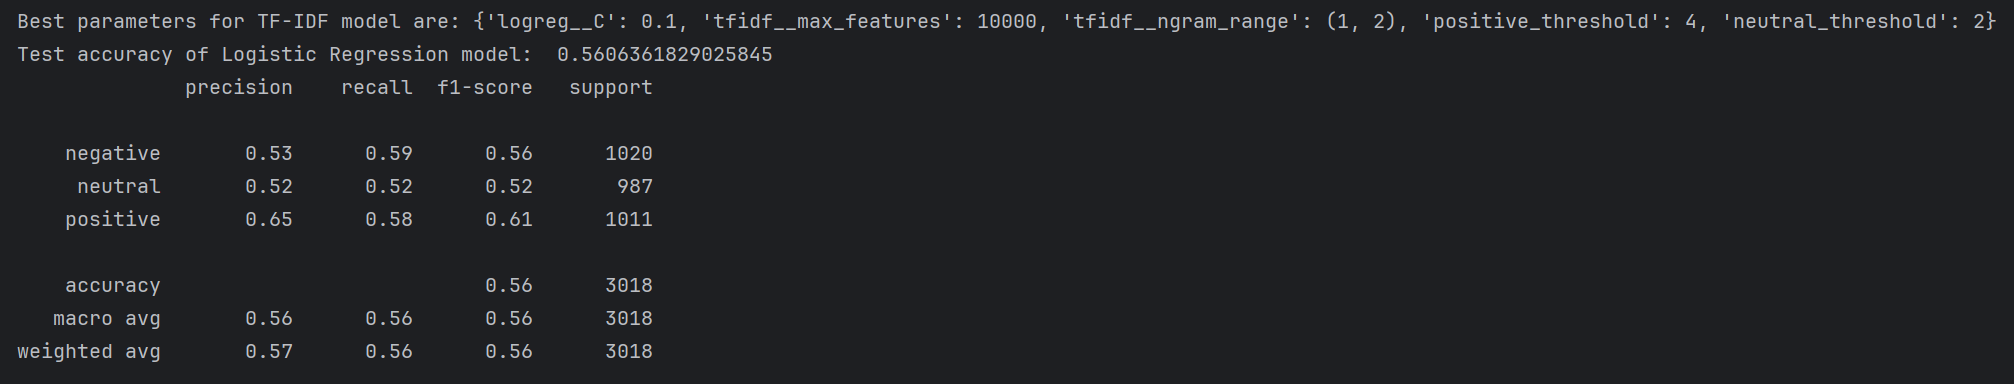
\includegraphics[width=0.5\textwidth]{img/70k_NoSW.png}
\end{figure}



\begin{figure}[h!]
    \caption{Confusion Matrix}
    \centering
    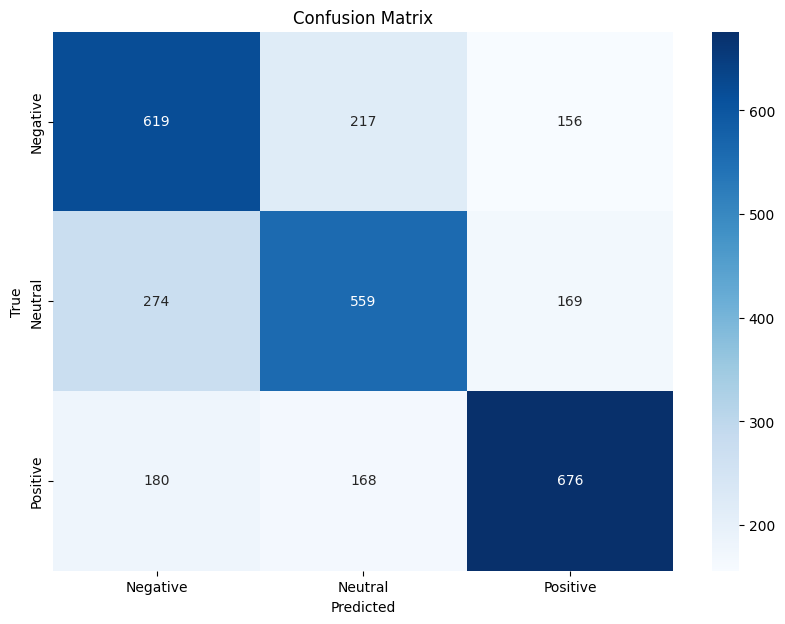
\includegraphics[width=0.5\textwidth]{img/conf.png}
\end{figure}


And the Final Result is as follows:

\begin{verbatim}
    Classification Report:
    precision    recall  f1-score      support
Negative       0.576887  0.623992  0.599516   992.000000
Neutral        0.592161  0.557884  0.574512  1002.000000
Positive       0.675325  0.660156  0.667654  1024.000000
accuracy       0.614314  0.614314  0.614314     0.614314
macro avg      0.614791  0.614011  0.613894  3018.000000
weighted avg   0.615358  0.614314  0.614333  3018.000000

Overall Metrics:
Accuracy: 0.6143
Precision: 0.6154
Recall: 0.6143
F1 Score: 0.6143
\end{verbatim}

\section{Document Classifier -  Transfomer Model}

The Transformer model is in \co{DocClassifier\_transformer.ipynb}. We investigate each segment in the following sections.

The first part of code is simply loading data and doing simple stuff like droping missing values.


\begin{lstlisting}[language=Python]
    # Import required packages
    import numpy as np
    import pandas as pd
    from sklearn.model_selection import train_test_split
    from sklearn.metrics import classification_report
    from sklearn.metrics import f1_score
    from sklearn.utils import shuffle
    import hazm
    from cleantext import clean
    import plotly.express as px
    import plotly.graph_objects as go
    from tqdm.notebook import tqdm
    import os
    import re
    import json
    import copy
    import collections
    import seaborn as sns
    import matplotlib.pyplot as plt
    from sklearn.metrics import classification_report, confusion_matrix, accuracy_score, precision_score, recall_score, f1_score
    from transformers import BertConfig, BertTokenizer
    from transformers import TFBertModel, TFBertForSequenceClassification
    from transformers import glue_convert_examples_to_features
    import tensorflow as tf
    
    # Import the pandas library for data manipulation and analysis
    import pandas as pd
    
    # Load the CSV file into a DataFrame
    data = pd.read_csv('/kaggle/input/taghchemain/taghche.csv')
    
    # Select only the 'comment' and 'rate' columns for further analysis
    data = data[['comment', 'rate']]
    
    # Display the first 10 rows of the DataFrame to get an overview of the data
    data.head(10)
    
    # Print the general information about the DataFrame
    print('data information')
    print(data.info(), '\n')
    
    # Print the statistics of missing values in the DataFrame
    print('missing values stats')
    print(data.isnull().sum(), '\n')
    
    # Print the first 5 rows where the 'rate' column has missing values
    print('some missing values')
    print(data[data['rate'].isnull()].iloc[:5], '\n')
    
    
    # Handle conflicts in the dataset structure
    # For simplicity, remove invalid data combinations
    
    # Replace ratings that are 6 or higher with None
    # This assumes that valid ratings should be between 0 and 5
    data['rate'] = data['rate'].apply(lambda r: r if r < 6 else None)
    
    # Drop rows where the 'rate' column has missing values
    data = data.dropna(subset=['rate'])
    
    # Drop rows where the 'comment' column has missing values
    data = data.dropna(subset=['comment'])
    
    # Remove duplicate comments, keeping only the first occurrence
    data = data.drop_duplicates(subset=['comment'], keep='first')
    
    # Reset the index of the DataFrame
    data = data.reset_index(drop=True)
    
    # Print the general information about the DataFrame
    print('data information')
    print(data.info(), '\n')
    
    # Print the statistics of missing values in the DataFrame
    print('missing values stats')
    print(data.isnull().sum(), '\n')
    
    # Print the first 5 rows where the 'rate' column has missing values
    print('some missing values')
    print(data[data['rate'].isnull()].iloc[:5], '\n')
\end{lstlisting}


\subsection*{Preprocess}



\begin{solution}
    \subsection*{Preprocessing}

    The comments have different lengths based on words. Detecting the most normal range could help us find the maximum length of the sequences for the preprocessing step. On the other hand, we suppose that the minimum word combination for having a meaningful phrase for our learning process is 1.
    
    \begin{lstlisting}[language=Python, basicstyle=\ttfamily\footnotesize, keywordstyle=\color{blue}, commentstyle=\color{gray}]
    # Calculate the length of comments based on the number of words
    # This uses hazm's word_tokenize function to split comments into words and then counts the number of words
    data['comment_len_by_words'] = data['comment'].apply(lambda t: len(hazm.word_tokenize(t)))
    
    # Determine the minimum and maximum comment lengths
    # This provides insights into the range of comment lengths in the dataset
    min_max_len = data["comment_len_by_words"].min(), data["comment_len_by_words"].max()
    
    # Print the minimum and maximum comment lengths
    # This helps understand the variation in comment lengths
    print(f'Min: {min_max_len[0]} \tMax: {min_max_len[1]}')
    \end{lstlisting}
    
    First, the code calculates the length of each comment based on the number of words. It uses the \texttt{word\_tokenize} function from the \texttt{hazm} library to split comments into words. The minimum and maximum lengths of the comments are then determined and printed to understand the variation in comment lengths.
    
    \begin{lstlisting}[language=Python, basicstyle=\ttfamily\footnotesize, keywordstyle=\color{blue}, commentstyle=\color{gray}]
    def data_gl_than(data, less_than=100.0, greater_than=0.0, col='comment_len_by_words'):
        """
        Calculate the percentage of comments with lengths greater than 'greater_than' and less than or equal to 'less_than'.
    
        Parameters:
        data (DataFrame): The DataFrame containing the data.
        less_than (float): The upper bound for the comment length.
        greater_than (float): The lower bound for the comment length.
        col (str): The column name that contains the comment lengths.
    
        Returns:
        None
        """
        # Extract the lengths of the comments from the specified column
        data_length = data[col].values
    
        # Count the number of comments that have a length greater than 'greater_than' and less than or equal to 'less_than'
        data_glt = sum([1 for length in data_length if greater_than < length <= less_than])
    
        # Calculate the percentage of such comments relative to the total number of comments
        data_glt_rate = (data_glt / len(data_length)) * 100
    
        # Print the result
        print(f'Texts with word length of greater than {greater_than} and less than {less_than} includes {data_glt_rate:.2f}% of the whole!')
    
    # Call the function with specific bounds
    data_gl_than(data, 256, 0)
    \end{lstlisting}
    
    The function \texttt{data\_gl\_than} calculates the percentage of comments with lengths greater than a specified lower bound and less than or equal to an upper bound. This is used to analyze the distribution of comment lengths within a specified range.
    
    \begin{lstlisting}[language=Python, basicstyle=\ttfamily\footnotesize, keywordstyle=\color{blue}, commentstyle=\color{gray}]
    # Define minimum and maximum limits for comment length
    minlim, maxlim = 0, 256
    
    # Remove comments with a length of fewer than three words or more than 256 words
    data['comment_len_by_words'] = data['comment_len_by_words'].apply(lambda len_t: len_t if minlim < len_t <= maxlim else None)
    
    # Drop rows where the 'comment_len_by_words' column has missing values
    data = data.dropna(subset=['comment_len_by_words'])
    
    # Reset the index of the DataFrame
    data = data.reset_index(drop=True)
    \end{lstlisting}
    
    Comments with a length of fewer than three words or more than 256 words are removed. The DataFrame is then updated to drop rows with missing values in the \texttt{comment\_len\_by\_words} column, and the index is reset.
    
    \begin{lstlisting}[language=Python, basicstyle=\ttfamily\footnotesize, keywordstyle=\color{blue}, commentstyle=\color{gray}]
    # This initializes an empty figure to which we will add traces
    fig = go.Figure()
    
    # Add a histogram trace to the figure
    # The x-axis data is taken from the 'comment_len_by_words' column
    fig.add_trace(go.Histogram(
        x=data['comment_len_by_words'],
        marker=dict(
            color='rgb(0, 123, 255)',  # Set bar color to a blue shade
            line=dict(
                color='rgb(8, 48, 107)',  # Set bar border color to a darker blue
                width=1.5,  # Set the width of the bar borders
            ),
        ),
        opacity=0.75,  # Set the opacity of the bars for a slight transparency effect
    ))
    
    # Update the layout of the figure
    # This includes setting titles for the plot and axes, and customizing the appearance
    fig.update_layout(
        title=dict(
            text='Distribution of Word Counts Within Comments',  # Set the title of the plot
            font=dict(size=24),  # Set the font size of the title
            x=0.5,  # Center the title on the plot
        ),
        xaxis=dict(
            title=dict(
                text='Word Count',  # Set the x-axis title
                font=dict(size=18),  # Set the font size of the x-axis title
            ),
            tickfont=dict(size=14),  # Set the font size of the x-axis tick labels
        ),
        yaxis=dict(
            title=dict(
                text='Frequency',  # Set the y-axis title
                font=dict(size=18),  # Set the font size of the y-axis title
            ),
            tickfont=dict(size=14),  # Set the font size of the y-axis tick labels
        ),
        bargap=0.2,  # Set the gap between individual bars
        bargroupgap=0.2,  # Set the gap between groups of bars
        template='plotly_white'  # Use the 'plotly_white' template for a cleaner look
    )
    
    # Show the figure
    fig.show()
    \end{lstlisting}
    
    A histogram is created to visualize the distribution of word counts within comments. The layout of the figure is customized, including setting titles for the plot and axes, and using the \texttt{plotly\_white} template for a cleaner look. The figure is then displayed.
    
    \begin{lstlisting}[language=Python, basicstyle=\ttfamily\footnotesize, keywordstyle=\color{blue}, commentstyle=\color{gray}]
    # Extract unique 'rate' values from the 'data' DataFrame, sort them, and convert them into a list
    unique_rates = list(sorted(data['rate'].unique()))
    
    # Print the number of unique rates and the list of unique rates
    print(f'We have {len(unique_rates)} unique rates: {unique_rates}')
    
    
    # Create a figure for the plot
    fig = go.Figure()
    
    # Group the data by 'rate' and count the occurrences of each rate
    groupby_rate = data.groupby('rate')['rate'].count()
    
    # Add a bar trace to the figure
    fig.add_trace(go.Bar(
        x=list(sorted(groupby_rate.index)),  # Set the x-axis data to the sorted unique rates
        y=groupby_rate.tolist(),  # Set the y-axis data to the frequency counts of each rate
        text=groupby_rate.tolist(),  # Display the frequency counts as text on the bars
        textposition='auto',  # Automatically position the text within the bars
        marker=dict(
            color='rgb(255, 123, 0)',  # Set bar color to an orange shade
            line=dict(
                color='rgb(107, 48, 8)',  # Set bar border color to a darker orange/brown
                width=1.5,  # Set the width of the bar borders
            ),
        ),
        opacity=0.75  # Set the opacity of the bars for a slight transparency effect
    ))
    
    # Update the layout of the figure
    # This includes titles for the plot and axes, as well as setting bar gaps
    fig.update_layout(
        title=dict(
            text='Distribution of Rates Within Comments',  # Set the title of the plot
            font=dict(size=24),  # Set title font size
            x=0.5,  # Center the title
        ),
        xaxis=dict(
            title=dict(
                text='Rate',  # Set the x-axis title
                font=dict(size=18),  # Set x-axis title font size
            ),
            tickfont=dict(size=14),  # Set x-axis tick font size
        ),
        yaxis=dict(
            title=dict(
                text='Frequency',  # Set the y-axis title
                font=dict(size=18),  # Set y-axis title font size
            ),
            tickfont=dict(size=14),  # Set y-axis tick font size
        ),
        bargap=0.2,  # Set the gap between individual bars
        bargroupgap=0.2,  # Set the gap between groups of bars
        template='plotly_white'  # Set the plot template for a cleaner look
    )
    
    # Show the figure
    fig.show()
    \end{lstlisting}
    
    A bar chart is created to visualize the distribution of rates within comments. The layout of the figure is customized, including setting titles for the plot and axes, and using the \texttt{plotly\_white} template for a cleaner look. The figure is then displayed.
    
    \begin{lstlisting}[language=Python, basicstyle=\ttfamily\footnotesize, keywordstyle=\color{blue}, commentstyle=\color{gray}]
    # Function to label the sentiment based on rating thresholds
    def label_sentiment(rate, positive_threshold, neutral_threshold):
        """
        Labels sentiment based on rating thresholds.
    
        Args:
        - rate (int or float): The numerical rating to evaluate.
        - positive_threshold (int or float): The minimum rating value that qualifies as 'positive'.
        - neutral_threshold (int or float): The minimum rating value that qualifies as 'neutral'; ratings below this are considered 'negative'.
    
        Returns:
        - str: The sentiment label ('positive', 'neutral', or 'negative') based on the rating.
        """
        # Check if the rating is greater than or equal to the positive threshold
        if rate >= positive_threshold:
            return 'positive'
        # If the rating is not 'positive', check if it is greater than or equal to the neutral threshold
        elif rate >= neutral_threshold:
            return 'neutral'
        # If the rating is neither 'positive' nor 'neutral', label the sentiment as 'negative'
        else:
            return 'negative'
        
    # Apply the label_sentiment function to the 'rate' column to create a new 'label' column
    data['label'] = data['rate'].apply(lambda t: label_sentiment(t, 4.0, 2.0))
    # Print unique labels
    labels = list(sorted(data['label'].unique()))
    # Display the first 5 rows of the DataFrame to get an overview of the data
    data.head()
    \end{lstlisting}
    
    The function \texttt{label\_sentiment} is defined to label the sentiment based on rating thresholds. Ratings are classified as \textit{positive}, \textit{neutral}, or \textit{negative} based on specified thresholds. The function is applied to the \texttt{rate} column to create a new \texttt{label} column.
    
    \begin{lstlisting}[language=Python, basicstyle=\ttfamily\footnotesize, keywordstyle=\color{blue}, commentstyle=\color{gray}]
    def preprocess(text):
        """
        Preprocess and normalize the given text string by performing several transformations.
        
        Args:
        text (str): The text string to be preprocessed.
        
        Returns:
        str: The preprocessed and normalized text string.
        """
        # Define a regular expression pattern that matches one or more newline characters
        pattern = re.compile(r"\n+")
        
        # Replace multiple newlines with a single newline
        text = pattern.sub("\n", text)
        
        # Remove special characters and replace newline characters with spaces
        text = re.sub(r'\\n|\n', ' ', text)
        
        # Remove non-Persian characters and digits
        text = re.sub(r'[^آ-ی\s\u200c]', ' ', text)
        
        # Define a regular expression pattern that matches one or more spaces
        pattern = re.compile(r" +")
        
        # Replace multiple spaces with a single space
        text = pattern.sub(" ", text)
        
        return text
    
    # Apply the preprocess function to the 'comment' column of the DataFrame
    data['cleaned_comment'] = data['comment'].apply(preprocess)
    
    # Remove duplicate rows from the DataFrame
    data = data.drop_duplicates()
    
    # Drop rows with empty or NaN values in the 'comment' or 'rate' columns
    data.dropna(subset=['comment', 'rate'], inplace=True)
    
    # Display the first 10 rows of the cleaned DataFrame
    data.head(10)
    \end{lstlisting}
    
    The function \texttt{preprocess} is defined to preprocess and normalize the text. It performs several transformations, including replacing multiple newlines with a single newline, removing special characters, and removing non-Persian characters and digits. The function is applied to the \texttt{comment} column. Duplicate rows are removed from the DataFrame, and rows with empty or NaN values in the \texttt{comment} or \texttt{rate} columns are dropped.

    

    \begin{lstlisting}[language=Python, basicstyle=\ttfamily\footnotesize, keywordstyle=\color{blue}, commentstyle=\color{gray}]
        # Create a figure for the plot
        fig = go.Figure()
        
        # Group the data by 'label' and count the occurrences of each label
        groupby_label = data.groupby('label')['label'].count()
        
        # Add a bar trace to the figure
        fig.add_trace(go.Bar(
            x=list(sorted(groupby_label.index)),  # Set the x-axis data to the sorted unique labels
            y=groupby_label.tolist(),  # Set the y-axis data to the frequency counts of each label
            text=groupby_label.tolist(),  # Display the frequency counts as text on the bars
            textposition='auto',  # Automatically position the text within the bars
            marker=dict(
                color='rgb(0, 123, 255)',  # Set bar color to a blue shade
                line=dict(
                    color='rgb(8, 48, 107)',  # Set bar border color to a darker blue
                    width=1.5,  # Set the width of the bar borders
                ),
            ),
            opacity=0.75  # Set the opacity of the bars for a slight transparency effect
        ))
        
        # Update the layout of the figure
        fig.update_layout(
            title=dict(
                text='Distribution of Labels Within Comments',  # Set the title of the plot
                font=dict(size=24),  # Set title font size
                x=0.5,  # Center the title
            ),
            xaxis=dict(
                title=dict(
                    text='Label',  # Set the x-axis title
                    font=dict(size=18),  # Set x-axis title font size
                ),
                tickfont=dict(size=14),  # Set x-axis tick font size
            ),
            yaxis=dict(
                title=dict(
                    text='Frequency',  # Set the y-axis title
                    font=dict(size=18),  # Set y-axis title font size
                ),
                tickfont=dict(size=14),  # Set y-axis tick font size
            ),
            bargap=0.2,  # Set the gap between individual bars
            bargroupgap=0.2,  # Set the gap between groups of bars
            template='plotly_white'  # Set the plot template for a cleaner look
        )
        
        # Show the figure
        fig.show()
        \end{lstlisting}
        
        The code creates a bar chart to visualize the distribution of sentiment labels within the comments. The layout is customized, and the plot is displayed.
        
        \subsection*{Balancing the Labels via Resampling}
        
        \begin{lstlisting}[language=Python, basicstyle=\ttfamily\footnotesize, keywordstyle=\color{blue}, commentstyle=\color{gray}]
        # Filter data into separate DataFrames based on 'label' values
        negative_data = data[data['label'] == 'negative']
        positive_data = data[data['label'] == 'positive']
        neutral_data = data[data['label'] == 'neutral']
        
        # Determine the smallest length among the three filtered DataFrames
        cutting_point = min(len(negative_data), len(positive_data), len(neutral_data))
        
        # If the cutting_point is less than or equal to the length of negative_data, sample down negative_data
        if cutting_point <= len(negative_data):
            negative_data = negative_data.sample(n=cutting_point).reset_index(drop=True)
        
        # If the cutting_point is less than or equal to the length of positive_data, sample down positive_data
        if cutting_point <= len(positive_data):
            positive_data = positive_data.sample(n=cutting_point).reset_index(drop=True)
        
        # If the cutting_point is less than or equal to the length of neutral_data, sample down neutral_data
        if cutting_point <= len(neutral_data):
            neutral_data = neutral_data.sample(n=cutting_point).reset_index(drop=True)
        
        # Concatenate the sampled DataFrames back into a single DataFrame
        new_data = pd.concat([negative_data, positive_data, neutral_data])
        
        # Shuffle the rows of the new DataFrame
        new_data = new_data.sample(frac=1).reset_index(drop=True)
        
        # Display summary information about the new DataFrame
        new_data.info()
        \end{lstlisting}
        
        The code balances the dataset by resampling each sentiment label to have an equal number of samples. This is done by determining the smallest length among the sentiment labels and sampling down the other labels to match this length. The DataFrames are concatenated, and the rows are shuffled.
        
        \subsection*{Distribution of Labels Within Comments After Balancing}
        
        \begin{lstlisting}[language=Python, basicstyle=\ttfamily\footnotesize, keywordstyle=\color{blue}, commentstyle=\color{gray}]
        # Create a figure for the plot
        fig = go.Figure()
        
        # Group the data by 'label' and count the occurrences of each label
        groupby_label = new_data.groupby('label')['label'].count()
        
        # Add a bar trace to the figure
        fig.add_trace(go.Bar(
            x=list(sorted(groupby_label.index)),  # Set the x-axis data to the sorted unique labels
            y=groupby_label.tolist(),  # Set the y-axis data to the frequency counts of each label
            text=groupby_label.tolist(),  # Display the frequency counts as text on the bars
            textposition='auto',  # Automatically position the text within the bars
            marker=dict(
                color='rgb(0, 123, 255)',  # Set bar color to a blue shade
                line=dict(
                    color='rgb(8, 48, 107)',  # Set bar border color to a darker blue
                    width=1.5,  # Set the width of the bar borders
                ),
            ),
            opacity=0.75  # Set the opacity of the bars for a slight transparency effect
        ))
        
        # Update the layout of the figure
        fig.update_layout(
            title=dict(
                text='Distribution of Labels Within Comments After Balancing Labels via Resampling',  # Set the title of the plot
                font=dict(size=24),  # Set title font size
                x=0.5,  # Center the title
            ),
            xaxis=dict(
                title=dict(
                    text='Label',  # Set the x-axis title
                    font=dict(size=18),  # Set x-axis title font size
                ),
                tickfont=dict(size=14),  # Set x-axis tick font size
            ),
            yaxis=dict(
                title=dict(
                    text='Frequency',  # Set the y-axis title
                    font=dict(size=18),  # Set y-axis title font size
                ),
                tickfont=dict(size=14),  # Set y-axis tick font size
            ),
            bargap=0.2,  # Set the gap between individual bars
            bargroupgap=0.2,  # Set the gap between groups of bars
            template='plotly_white'  # Set the plot template for a cleaner look
        )
        
        # Show the figure
        fig.show()
        \end{lstlisting}
        
        A second bar chart is created to visualize the distribution of sentiment labels within the comments after balancing the dataset via resampling. The layout is customized, and the plot is displayed.

\end{solution}




\subsection*{Training Configuration}



\begin{solution}

    \subsection*{Mapping Labels to Numerical IDs and Data Splitting}

    \begin{lstlisting}[language=Python, basicstyle=\ttfamily\footnotesize, keywordstyle=\color{blue}, commentstyle=\color{gray}]
    # Map labels to numerical ids and add a new column 'label_id' to new_data
    new_data['label_id'] = new_data['label'].apply(lambda t: labels.index(t))
    
    # Split new_data into train and test sets (80% train, 20% test), stratified by 'label'
    train, test = train_test_split(new_data, test_size=0.2, random_state=1, stratify=new_data['label'])
    
    # Further split test set into test and validation sets (50% test, 50% validation), stratified by 'label'
    test, valid = train_test_split(test, test_size=0.5, random_state=1, stratify=test['label'])
    
    # Reset index for train, validation, and test sets to ensure continuous integer indices
    train = train.reset_index(drop=True)
    valid = valid.reset_index(drop=True)
    test = test.reset_index(drop=True)
    
    # Extract comments and label_ids for train, validation, and test sets
    x_train, y_train = train['comment'].values.tolist(), train['label_id'].values.tolist()
    x_valid, y_valid = valid['comment'].values.tolist(), valid['label_id'].values.tolist()
    x_test, y_test = test['comment'].values.tolist(), test['label_id'].values.tolist()
    
    # Print shapes of train, validation, and test sets to verify sizes
    print(train.shape)
    print(valid.shape)
    print(test.shape)
    \end{lstlisting}
    
    The code maps the text labels to numerical IDs and adds a new column 'label\_id' to the DataFrame. The data is then split into train (80\%), test (20\%), and validation (50\% of the test set) sets, ensuring stratification by label to maintain the distribution of classes in each subset. The indices of each set are reset, and the comments and label IDs are extracted for each set. Finally, the shapes of the train, validation, and test sets are printed to verify the sizes.
    
    \subsection*{Configuration Parameters for BERT Model Training}
    
    \begin{lstlisting}[language=Python, basicstyle=\ttfamily\footnotesize, keywordstyle=\color{blue}, commentstyle=\color{gray}]
    # General configuration parameters
    MAX_LEN = 128              # Maximum sequence length
    TRAIN_BATCH_SIZE = 64      # Batch size for training
    VALID_BATCH_SIZE = 64      # Batch size for validation
    TEST_BATCH_SIZE = 64       # Batch size for testing
    
    EPOCHS = 3                 # Number of epochs for training
    EVERY_EPOCH = 1000        # Number of steps to print progress during each epoch
    LEARNING_RATE = 2e-5       # Learning rate for the optimizer
    CLIP = 0.0                 # Gradient clipping threshold
    
    MODEL_NAME_OR_PATH = 'HooshvareLab/bert-fa-base-uncased'  # Pre-trained model name or path
    OUTPUT_PATH = '/content/bert-fa-base-uncased-sentiment-taaghceh/pytorch_model.bin'  # Path to save the trained model
    
    # Create the directory to save the trained model if it does not exist
    os.makedirs(os.path.dirname(OUTPUT_PATH), exist_ok=True)
    \end{lstlisting}
    
    The general configuration parameters for training the BERT model are defined. This includes the maximum sequence length, batch sizes for training, validation, and testing, the number of epochs, learning rate, gradient clipping threshold, the pre-trained model path, and the path to save the trained model. The output directory is created if it does not already exist.
    
    \subsection*{Label Mapping Dictionaries and BERT Configuration}
    
    \begin{lstlisting}[language=Python, basicstyle=\ttfamily\footnotesize, keywordstyle=\color{blue}, commentstyle=\color{gray}]
    # Create a dictionary mapping labels to numerical ids
    label2id = {label: i for i, label in enumerate(labels)}
    
    # Create a dictionary mapping numerical ids back to labels
    id2label = {v: k for k, v in label2id.items()}
    
    # Print label2id dictionary
    print(f'label2id: {label2id}')
    
    # Print id2label dictionary
    print(f'id2label: {id2label}')
    
    # Initialize a BERT tokenizer using the pre-trained model specified in MODEL_NAME_OR_PATH
    tokenizer = BertTokenizer.from_pretrained(MODEL_NAME_OR_PATH, force_download=True)
    
    # Create a BERT configuration object using the pre-trained model and additional custom settings
    config = BertConfig.from_pretrained(
        MODEL_NAME_OR_PATH,  # Specify the pre-trained model name or path
        **{                  # Additional custom settings passed as keyword arguments
            'label2id': label2id,  # Mapping from labels to numerical ids
            'id2label': id2label   # Mapping from numerical ids back to labels
        })
    
    # Print the configuration details in JSON format
    print(config.to_json_string())
    \end{lstlisting}
    
    Label mapping dictionaries are created to map labels to numerical IDs and vice versa. These mappings are printed for verification. A BERT tokenizer and configuration object are initialized using the specified pre-trained model path and the custom label mappings. The configuration details are printed in JSON format.
    

\end{solution}




\subsection*{Input Embedding and Training}


\begin{solution}
    \subsection*{Preparing Datasets for BERT Model Training}

    \begin{lstlisting}[language=Python, basicstyle=\ttfamily\footnotesize, keywordstyle=\color{blue}, commentstyle=\color{gray}]
    import tensorflow as tf
    import numpy as np
    from tqdm import tqdm
    from transformers import glue_convert_examples_to_features
    
    class InputExample:
        """ A single example for simple sequence classification. """
        
        def __init__(self, guid, text_a, text_b=None, label=None):
            """ Constructs an InputExample. """
            self.guid = guid
            self.text_a = text_a
            self.text_b = text_b
            self.label = label
    
    def make_examples(tokenizer, x, y=None, maxlen=128, output_mode="classification", is_tf_dataset=True):
        """
        Converts input texts and labels into examples and features suitable for BERT model training.
    
        Args:
        tokenizer (transformers.PreTrainedTokenizer): Tokenizer object for tokenizing input texts.
        x (list): List of input texts or tuples of input texts (for sequence classification).
        y (list, optional): List of labels corresponding to input texts. Default is None.
        maxlen (int, optional): Maximum sequence length for input texts. Default is 128.
        output_mode (str, optional): Output mode for the task (e.g., "classification"). Default is "classification".
        is_tf_dataset (bool, optional): Whether to return a TensorFlow dataset or numpy arrays. Default is True.
    
        Returns:
        tf.data.Dataset or tuple of numpy arrays: Depending on is_tf_dataset, returns either a TensorFlow dataset
                                                 or a tuple of numpy arrays containing input_ids, attention_masks,
                                                 token_type_ids, and labels.
        list: List of features converted from InputExamples.
        """
        examples = []
        y = y if isinstance(y, list) or isinstance(y, np.ndarray) else [None] * len(x)
    
        # Create InputExamples from input texts and labels
        for i, (_x, _y) in tqdm(enumerate(zip(x, y)), position=0, total=len(x)):
            guid = "%s" % i
            label = int(_y)
    
            if isinstance(_x, str):
                text_a = _x
                text_b = None
            else:
                assert len(_x) == 2
                text_a = _x[0]
                text_b = _x[1]
    
            examples.append(InputExample(guid=guid, text_a=text_a, text_b=text_b, label=label))
    
        # Convert InputExamples to features using glue_convert_examples_to_features function
        features = glue_convert_examples_to_features(
            examples,
            tokenizer,
            maxlen,
            output_mode=output_mode,
            label_list=list(np.unique(y)))
    
        all_input_ids = []
        all_attention_masks = []
        all_token_type_ids = []
        all_labels = []
    
        # Process features into input arrays for TensorFlow dataset or numpy arrays
        for f in tqdm(features, position=0, total=len(examples)):
            if is_tf_dataset:
                all_input_ids.append(tf.constant(f.input_ids))
                all_attention_masks.append(tf.constant(f.attention_mask))
                all_token_type_ids.append(tf.constant(f.token_type_ids))
                all_labels.append(tf.constant(f.label))
            else:
                all_input_ids.append(f.input_ids)
                all_attention_masks.append(f.attention_mask)
                all_token_type_ids.append(f.token_type_ids)
                all_labels.append(f.label)
    
        if is_tf_dataset:
            # Create TensorFlow dataset from input arrays
            dataset = tf.data.Dataset.from_tensor_slices(({
                'input_ids': all_input_ids,
                'attention_mask': all_attention_masks,
                'token_type_ids': all_token_type_ids
            }, all_labels))
    
            return dataset, features
    
        # Return tuple of numpy arrays if is_tf_dataset=False
        xdata = [np.array(all_input_ids), np.array(all_attention_masks), np.array(all_token_type_ids)]
        ydata = all_labels
    
        return [xdata, ydata], features
    
    # Create training dataset and examples using make_examples function
    train_dataset_base, train_examples = make_examples(tokenizer, x_train, y_train, maxlen=128)
    
    # Create validation dataset and examples using make_examples function
    valid_dataset_base, valid_examples = make_examples(tokenizer, x_valid, y_valid, maxlen=128)
    
    # Create test dataset and examples using make_examples function
    test_dataset_base, test_examples = make_examples(tokenizer, x_test, y_test, maxlen=128)
    
    # Create test dataset and examples as numpy arrays (not TensorFlow dataset)
    [xtest, ytest], test_examples = make_examples(tokenizer, x_test, y_test, maxlen=128, is_tf_dataset=False)
    
    # Iterate over the first example in the train_dataset_base
    for value in train_dataset_base.take(1):
        # Print input_ids tensor
        print(f'     input_ids: {value[0]["input_ids"]}')
        # Print attention_mask tensor
        print(f'attention_mask: {value[0]["attention_mask"]}')
        # Print token_type_ids tensor
        print(f'token_type_ids: {value[0]["token_type_ids"]}')
        # Print target (label) tensor
        print(f'        target: {value[1]}')
    \end{lstlisting}
    
    The code defines an `InputExample` class for creating input examples for sequence classification and a `make\_examples` function to convert texts and labels into examples and features suitable for BERT model training. It creates TensorFlow datasets for training, validation, and testing, and prints the first example in the training dataset to verify correctness.
    
    \subsection*{Building and Training the BERT Model}
    
    \begin{lstlisting}[language=Python, basicstyle=\ttfamily\footnotesize, keywordstyle=\color{blue}, commentstyle=\color{gray}]
    def get_training_dataset(dataset, batch_size):
        """
        Creates a training dataset pipeline.
    
        Args:
        dataset (tf.data.Dataset): TensorFlow dataset containing training examples.
        batch_size (int): Batch size for training.
    
        Returns:
        tf.data.Dataset: Processed training dataset ready for model training.
        """
        # Repeat the dataset indefinitely
        dataset = dataset.repeat()
        # Shuffle the dataset with a buffer size of 2048
        dataset = dataset.shuffle(2048)
        # Batch the dataset with the specified batch size
        dataset = dataset.batch(batch_size)
    
        return dataset
    
    def get_validation_dataset(dataset, batch_size):
        """
        Creates a validation dataset pipeline.
    
        Args:
        dataset (tf.data.Dataset): TensorFlow dataset containing validation examples.
        batch_size (int): Batch size for validation.
    
        Returns:
        tf.data.Dataset: Processed validation dataset ready for model evaluation.
        """
        # Batch the dataset with the specified batch size
        dataset = dataset.batch(batch_size)
    
        return dataset
    
    # Create training dataset using get_training_dataset function
    train_dataset = get_training_dataset(train_dataset_base, TRAIN_BATCH_SIZE)
    
    # Create validation dataset using get_validation_dataset function
    valid_dataset = get_validation_dataset(valid_dataset_base, VALID_BATCH_SIZE)
    
    # Calculate steps per epoch for training and validation
    train_steps = len(train_examples) // TRAIN_BATCH_SIZE
    valid_steps = len(valid_examples) // VALID_BATCH_SIZE
    
    # Print the calculated steps for training and validation
    print(train_steps, valid_steps)
    
    def build_model(model_name, config, learning_rate=3e-5):
        """
        Builds a TensorFlow model for sequence classification using a pre-trained BERT model.
    
        Args:
        model_name (str): Pre-trained model name or path.
        config (transformers.PretrainedConfig): Configuration object for the BERT model.
        learning_rate (float, optional): Learning rate for optimizer. Default is 3e-5.
    
        Returns:
        tf.keras.Model: Compiled BERT-based model for sequence classification.
        """
        # Load pre-trained BERT model for sequence classification
        model = TFBertForSequenceClassification.from_pretrained(model_name, force_download=True, config=config)
    
        # Define optimizer, loss function, and metrics for the model
        optimizer = tf.keras.optimizers.Adam(learning_rate=learning_rate)
        loss = tf.keras.losses.SparseCategoricalCrossentropy(from_logits=True)
        metric = tf.keras.metrics.SparseCategoricalAccuracy('accuracy')
    
        # Compile the model with optimizer, loss function, and metrics
        model.compile(optimizer=optimizer, loss=loss, metrics=[metric])
    
        return model
    
    # Build BERT-based model for sequence classification
    model = build_model(MODEL_NAME_OR_PATH, config, learning_rate=LEARNING_RATE)
    
    %%time
    
    # Train the BERT-based model
    r = model.fit(
        train_dataset,                           # Training dataset
        validation_data=valid_dataset,           # Validation dataset
        steps_per_epoch=train_steps,             # Number of steps per epoch for training
        batch_size=128,                          # Batch size for training
        validation_steps=valid_steps,            # Number of steps per epoch for validation
        epochs=EPOCHS,                           # Number of epochs
        verbose=1                                # Verbosity mode (1 for progress bar)
    )
    
    # Extract validation accuracy from training history
    final_accuracy = r.history['val_accuracy']
    print('FINAL ACCURACY MEAN: ', np.mean(final_accuracy))
    
    # Save the trained model
    model.save_pretrained(os.path.dirname(OUTPUT_PATH))
    \end{lstlisting}
    
    The `get\_training\_dataset` and `get\_validation\_dataset` functions create data pipelines for training and validation. The `build\_model` function builds and compiles a BERT-based model for sequence classification. The model is then trained, and its validation accuracy is printed and the trained model is saved.
\end{solution}



\subsection{Results}

Results are generated using the following code



\begin{solution}
    \begin{lstlisting}[language=Python, basicstyle=\ttfamily\footnotesize, keywordstyle=\color{blue}, commentstyle=\color{gray}]
        def evaluate_model(y_true, y_pred, class_names):
            """
            Evaluates the performance of a classification model using various metrics and visualizations.
        
            Args:
            - y_true (array-like): True labels of the data.
            - y_pred (array-like): Predicted labels of the data.
            - class_names (list): List of class names in the same order as the confusion matrix.
        
            Returns:
            - pd.DataFrame: DataFrame containing the classification report.
            """
            # Generate and print the classification report
            report = classification_report(y_true, y_pred, target_names=class_names, output_dict=True)
            report_df = pd.DataFrame(report).transpose()
            print("Classification Report:\n", report_df)
        
            # Generate and display the confusion matrix as a heatmap
            cm = confusion_matrix(y_true, y_pred)
            plt.figure(figsize=(10, 7))
            sns.heatmap(cm, annot=True, fmt='d', cmap='Blues', xticklabels=class_names, yticklabels=class_names)
            plt.xlabel('Predicted')
            plt.ylabel('True')
            plt.title('Confusion Matrix')
            plt.show()
        
            # Calculate and print overall metrics: accuracy, precision, recall, and F1 score
            accuracy = accuracy_score(y_true, y_pred)
            precision = precision_score(y_true, y_pred, average='weighted')
            recall = recall_score(y_true, y_pred, average='weighted')
            f1 = f1_score(y_true, y_pred, average='weighted')
        
            metrics = {
                "Accuracy": accuracy,
                "Precision": precision,
                "Recall": recall,
                "F1 Score": f1
            }
        
            print("\nOverall Metrics:")
            for metric, value in metrics.items():
                print(f"{metric}: {value:.4f}")
            
            return report_df
        
        # Perform predictions on the test dataset
        predictions = model.predict(xtest)
        
        # Extract predicted labels from predictions
        ypred = predictions[0].argmax(axis=-1).tolist()
        
        # Evaluate the model
        report_df = evaluate_model(ytest, ypred, ["Negative", "Neutral", "Positive"])
        \end{lstlisting}
        
        The `evaluate\_model` function assesses the performance of a classification model using various metrics and visualizations. It generates a classification report, displays a confusion matrix as a heatmap, and calculates overall metrics such as accuracy, precision, recall, and F1 score. The function prints these metrics and returns the classification report as a DataFrame.
        
        The code performs predictions on the test dataset using the trained BERT model, extracts the predicted labels, and evaluates the model's performance by calling the `evaluate\_model` function. The function is provided with the true labels, predicted labels, and class names for evaluation.
        
        The following steps are performed:
        \begin{enumerate}
        \item The `evaluate\_model` function generates a classification report and displays it.
        \item A confusion matrix is generated and visualized as a heatmap.
        \item Overall metrics (accuracy, precision, recall, and F1 score) are calculated and printed.
        \item The classification report is returned as a DataFrame.
                \end{enumerate}
\end{solution}


\begin{figure}[h!]
    \caption{Results of running Transformer on Dataset}
    \centering
    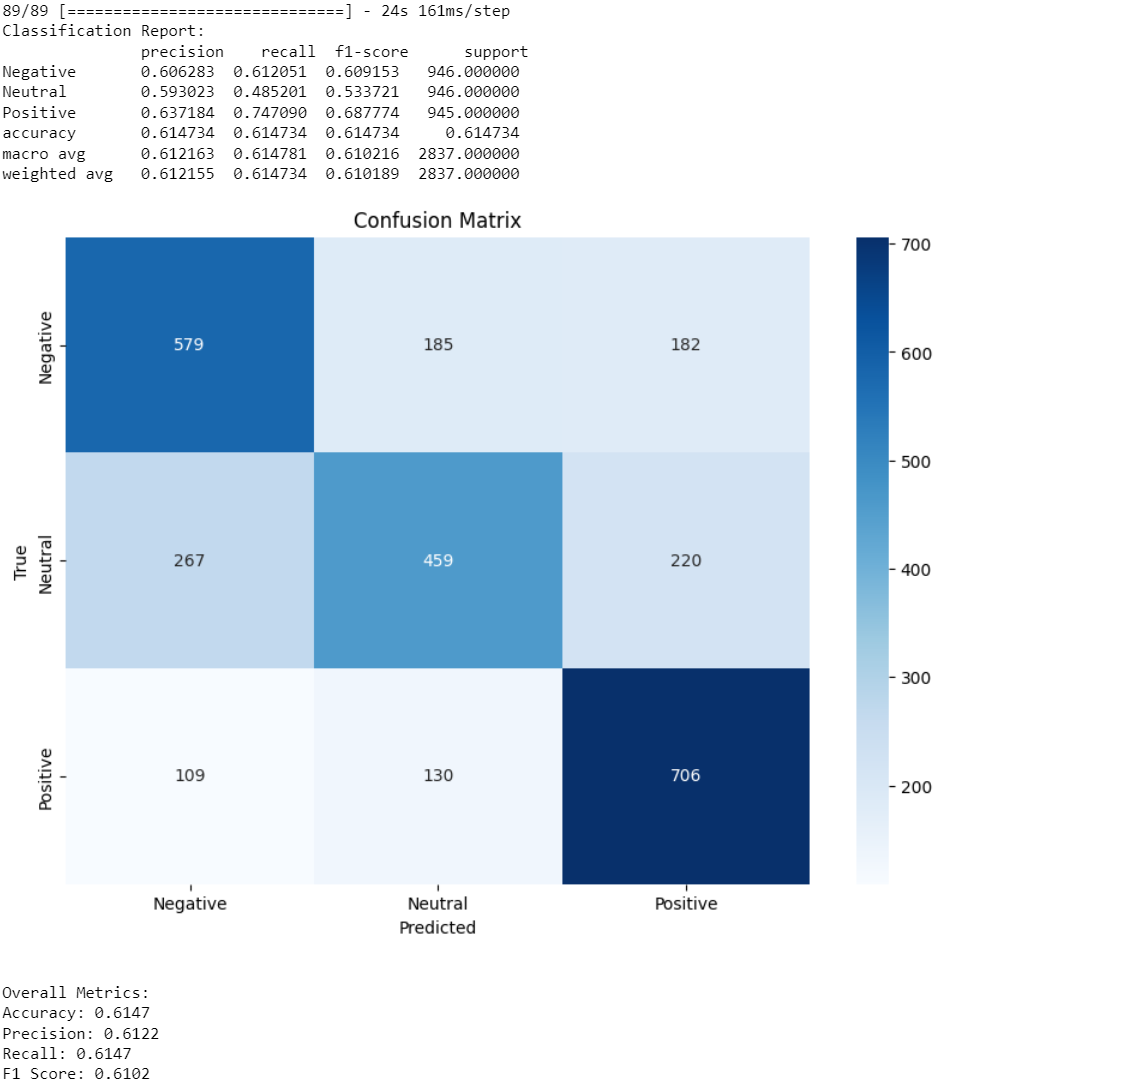
\includegraphics[width=0.5\textwidth]{img/transformer1.png}
\end{figure}



\section{Word Classifier - Base Model}
The base model is in \co{WordClassifier\_Base.ipynb}. We investigate each segment in the following sections.


\subsection*{Initial Preprocessing}



\begin{solution}

    \begin{lstlisting}
        prepared_data: pd.DataFrame = pd.read_csv(url + 'datasets/taghche.csv')
        prepared_data = prepared_data[['comment', 'bookname', 'bookID']]
        \end{lstlisting}
        
        The script reads a CSV file containing text data and selects specific columns: \texttt{comment}, \texttt{bookname}, and \texttt{bookID}.
        
        \begin{lstlisting}
        chars_stop_words = ''
        with open(url + 'stopwords/chars (without digits).txt', 'r', encoding='utf-8') as file:
            chars_stop_words = ''.join(file.read().splitlines())
        
        chars_stop_words = chars_stop_words.replace('[', '\[')
        chars_stop_words = chars_stop_words.replace(']', '\]')
        chars_pattern = re.compile(f'[{chars_stop_words}]')
        chars_pattern
        \end{lstlisting}
        
        The script reads a file containing stop words (characters to be removed) and creates a regular expression pattern to match these characters.
        
        \begin{lstlisting}
        emojis_pattern = re.compile("["
                                    u"\U0001F600-\U0001F64F"  # emoticons
                                    u"\U0001F300-\U0001F5FF"  # symbols & pictographs
                                    u"\U0001F680-\U0001F6FF"  # transport & map symbols
                                    u"\U0001F1E0-\U0001F1FF"  # flags (iOS)
                                    "]+")
        \end{lstlisting}
        
        The script defines a regular expression pattern to match emojis using Unicode ranges.
        
        \begin{lstlisting}
        def elementary_preprocess(text):
            global chars_pattern, emojis_pattern
        
            text = str(text)
            text = chars_pattern.sub(r' ', text)
            text = emojis_pattern.sub(r' ', text)
            return text.translate(str.maketrans('0123456789', '۰۱۲۳۴۵۶۷۸۹'))
        \end{lstlisting}
        
        The \texttt{elementary\_preprocess} function removes unwanted characters and emojis from the text and translates digits to Persian numerals.
        
        \begin{lstlisting}
        def higher_preprocess(text, is_informal=False):
            global normalizer
        
            text = str(text)
            
            if is_informal:
                text = informal_normalizer_function(text)
                # progress_bar.update(1)
            else:
                text = normalizer.normalize(text)
            
            text = word_tokenize(text)
            return text
        \end{lstlisting}
        
        The \texttt{higher\_preprocess} function normalizes the text. If \texttt{is\_informal} is \texttt{True}, it uses an informal normalizer; otherwise, it uses a standard normalizer. The function tokenizes the normalized text.
        
        \begin{lstlisting}
        def informal_normalizer_function(text):
            global informal_normalizer
            text = str(text)
        
            informal_normalizer = InformalNormalizer()
            text = Normalizer.normalize(informal_normalizer, text)
            sents = [
                informal_normalizer.word_tokenizer.tokenize(sentence)
                for sentence in informal_normalizer.sent_tokenizer.tokenize(text)
            ]
        
            normalized = [[informal_normalizer.normalized_word(word)[0] for word in sent] for sent in sents]
            normalized = np.array(normalized, dtype=object)
            return np.hstack(normalized)
        
        normalizer = Normalizer()
        informal_normalizer = InformalNormalizer()
        \end{lstlisting}
        
        The \texttt{informal\_normalizer\_function} customizes the normalization process for informal text. It tokenizes sentences and words, then normalizes each word.
        
        \begin{lstlisting}
        for column in prepared_data.columns:
            if column == 'bookID':
                continue
            
            print(f'Column: {column}')
            prepared_data[column] = prepared_data[column].progress_apply(elementary_preprocess)
        \end{lstlisting}
        
        The script applies the \texttt{elementary\_preprocess} function to each column of the data except \texttt{bookID}.
        
        \begin{lstlisting}
        for column in prepared_data.columns:
            if column == 'bookID':
                continue
            
            print(f'Column: {column}')
            prepared_data[column] = prepared_data[column].progress_apply(higher_preprocess)
        \end{lstlisting}
        
        Next, the script applies the \texttt{higher\_preprocess} function to each column of the data except \texttt{bookID}.
        
        \begin{lstlisting}
        before_dropping = len(prepared_data)
        prepared_data = prepared_data[prepared_data['comment'].apply(lambda x: len(x)) != 0]
        print(f'Dropped {before_dropping - len(prepared_data)} rows with empty comment.')
        
        before_dropping = len(prepared_data)
        prepared_data = prepared_data.dropna(subset=['bookID'])
        print(f'Dropped {before_dropping - len(prepared_data)} rows with NaN bookID.')
        \end{lstlisting}
        
        Finally, the script removes rows with empty comments and rows with missing \texttt{bookID} values, printing the number of dropped rows.
        
\end{solution}






\subsection*{Using Crawled Data}



\begin{solution}
    The following Python script processes and normalizes a dataset containing book data. It combines multiple CSV files into a single DataFrame, sorts and processes author names, removes duplicates and rows with missing IDs, and normalizes text data.

    \begin{lstlisting}
    ALL_PARTS_LEN = 19
    crawled_data: pd.DataFrame = pd.read_csv(url + 'datasets/books data/books_data_part_1.csv')
    for i in range(2, ALL_PARTS_LEN + 1):
        crawled_data = pd.concat([crawled_data, pd.read_csv(url + f'datasets/books data/books_data_part_{i}.csv')],
                                 ignore_index=True)
    \end{lstlisting}
    
    The script first reads the initial CSV file into a DataFrame called \texttt{crawled\_data}. It then iteratively reads and concatenates additional CSV files into this DataFrame. The variable \texttt{ALL\_PARTS\_LEN} determines the number of parts to be combined.
    
    \begin{lstlisting}
    new_author_function = lambda x: ' $ '.join(sorted(str(x).split(' $ ')))
    crawled_data['author'] = crawled_data['author'].apply(new_author_function)
    \end{lstlisting}
    
    This section of the code defines a lambda function to sort the author names within each entry. The authors are separated by the delimiter \texttt{' \$ '}. The lambda function sorts the names alphabetically and joins them back together with the same delimiter.
    
    \begin{lstlisting}
    before_dropping = len(crawled_data)
    crawled_data = crawled_data.drop_duplicates()
    print(f'Dropped {before_dropping - len(crawled_data)} duplicates.')
    \end{lstlisting}
    
    The script removes duplicate rows from \texttt{crawled\_data} and prints the number of duplicates dropped.
    
    \begin{lstlisting}
    before_dropping = len(crawled_data)
    crawled_data = crawled_data.dropna(subset=['id'])
    print(f'Dropped {before_dropping - len(crawled_data)} rows with NaN id.')
    \end{lstlisting}
    
    Rows with missing \texttt{id} values are dropped, and the number of such rows is printed.
    
    \begin{lstlisting}
    new_author_function = lambda x: set(x.split(' $ '))
    crawled_data['author'] = crawled_data['author'].apply(new_author_function)
    \end{lstlisting}
    
    The script redefines the lambda function to convert the list of authors into a set, effectively eliminating duplicate authors within each entry.
    
    \begin{lstlisting}
    crawled_data = crawled_data.explode('author')
    crawled_data = crawled_data.reset_index(drop=True)
    \end{lstlisting}
    
    The \texttt{explode} method is used to transform each author into a separate row, enabling independent processing of each author in the comments. The index is reset to maintain a clean DataFrame.
    
    \begin{lstlisting}
    for column in crawled_data.columns:
        if column == 'id':
            continue
        
        print(f'Column: {column}')
        crawled_data[column] = crawled_data[column].progress_apply(elementary_preprocess)
    \end{lstlisting}
    
    The script applies the \texttt{elementary\_preprocess} function to each column of the \texttt{crawled\_data} DataFrame, excluding the \texttt{id} column. This function removes unwanted characters and emojis and translates digits to Persian numerals.
    
    \begin{lstlisting}
    for column in crawled_data.columns:
        if column == 'id':
            continue
            
        print(f'Column: {column}')
        crawled_data[column] = crawled_data[column].progress_apply(higher_preprocess)
    \end{lstlisting}
    
    The script then applies the \texttt{higher\_preprocess} function to each column of the \texttt{crawled\_data} DataFrame, again excluding the \texttt{id} column. This function normalizes and tokenizes the text.
    


    The following Python script merges two datasets, identifies unavailable books, and saves a list of unavailable book IDs to a file. The datasets are preprocessed to remove duplicates and missing values before being merged.

\begin{lstlisting}
data: pd.DataFrame = pd.merge(prepared_data, crawled_data, left_on='bookID', right_on='id')
data = data.drop(columns=['bookID'])

print(f'Prepared data: {len(prepared_data)}\nCrawled data: {len(crawled_data)}\nMerged data: {len(data)}')
data.head()
\end{lstlisting}

The script merges the \texttt{prepared\_data} and \texttt{crawled\_data} DataFrames using a common key: \texttt{bookID} from \texttt{prepared\_data} and \texttt{id} from \texttt{crawled\_data}. After merging, the \texttt{bookID} column is dropped from the merged DataFrame. The script then prints the lengths of the prepared, crawled, and merged datasets and displays the first few rows of the merged dataset.

\begin{lstlisting}
crawled_books = set(crawled_data['id'].values)
prepared_books = prepared_data[['bookID']].copy()

unavailable_books = prepared_books[~prepared_books['bookID'].apply(lambda x: x in crawled_books)]
unavailable_books = unavailable_books.drop_duplicates()
print(f'Unavailable books (The page has 404 error): {len(unavailable_books)}')
unavailable_books
\end{lstlisting}

The script identifies books in the \texttt{prepared\_data} DataFrame that are not present in the \texttt{crawled\_data} DataFrame. It creates a set of book IDs from \texttt{crawled\_data} and compares it to the \texttt{bookID} column in \texttt{prepared\_data}. Books not found in \texttt{crawled\_data} are considered unavailable. The script removes duplicate entries and prints the number of unavailable books.

\begin{lstlisting}
with open('unavailable_books_list.txt', 'w', encoding='utf-8') as file:
    unavailable_books_list = unavailable_books['bookID'].values.flatten()
    unavailable_books_list = unavailable_books_list[~np.isnan(unavailable_books_list)]
    unavailable_books_list = unavailable_books_list.astype(int)
    unavailable_books_list = unavailable_books_list.tolist()
    unavailable_books_list = sorted(list(set(unavailable_books_list)))
    file.write(str(unavailable_books_list))
\end{lstlisting}

The script writes the list of unavailable book IDs to a text file. It flattens the array of book IDs, removes any NaN values, converts the IDs to integers, and sorts them. Finally, it saves the sorted list of unique unavailable book IDs to a file named \texttt{unavailable\_books\_list.txt}.

    
\end{solution}




\subsection*{Labeling}




\begin{solution}

    The following Python script processes a dataset to label parts of text related to books, authors, translators, and publishers. It then visualizes the distribution of these labels and removes rows with insufficient labels.

    \begin{lstlisting}
    labeled_data = data.copy()
    labeled_data['label'] = [[0]] * len(labeled_data)
    labeled_data.head()
    
    tags = ['name', 'author', 'translator', 'publisher']
    \end{lstlisting}
    
    The script begins by copying the \texttt{data} DataFrame to \texttt{labeled\_data} and initializes a new column, \texttt{label}, with zero values. It also defines a list of tags representing different entities in the dataset.
    
    \begin{lstlisting}
    def get_label(tag):
        if tag == 'name':
            return 'Book'
        elif tag == 'author':
            return 'Author'
        elif tag == 'translator':
            return 'Translator'
        elif tag == 'publisher':
            return 'Publisher'
        else:
            return None
    \end{lstlisting}
    
    The \texttt{get\_label} function maps each tag to its corresponding entity label. This function helps in converting tag names to more descriptive labels.
    
    \begin{lstlisting}
    def convert_index_to_label(index, tag):
        labels = []
    
        for i in range(len(index)):
            if index[i] == -1:
                labels.append('O')
            else:
                if i == 0 or index[i - 1] == -1 or index[i] - index[i - 1] != 1:
                    labels.append(f'B-{get_label(tag)}')
                else:
                    labels.append(f'I-{get_label(tag)}')
    
        return labels
    \end{lstlisting}
    
    The \texttt{convert\_index\_to\_label} function converts a list of indexes to labels. It uses the BIO (Beginning, Inside, Outside) tagging scheme to mark the beginning (\texttt{B-}) and continuation (\texttt{I-}) of entities. If the index is -1, it assigns the label \texttt{O} (Outside).
    
    \begin{lstlisting}
    def combine_labels(labels):
        global tags
    
        result = []
    
        for i in range(len(labels[tags[0]])):
            name = labels[tags[0]][i] if len(labels[tags[0]]) > 0 else 'O'
            author = labels[tags[1]][i] if len(labels[tags[1]]) > 0 else 'O'
            translator = labels[tags[2]][i] if len(labels[tags[2]]) > 0 else 'O'
            publisher = labels[tags[3]][i] if len(labels[tags[3]]) > 0 else 'O'
    
            if name != 'O':
                result.append(name)
            elif author != 'O':
                result.append(author)
            elif translator != 'O':
                result.append(translator)
            elif publisher != 'O':
                result.append(publisher)
            else:
                result.append('O')
    
        return result
    \end{lstlisting}
    
    The \texttt{combine\_labels} function combines labels for different tags into a single list. It prioritizes the \texttt{name} tag, followed by \texttt{author}, \texttt{translator}, and \texttt{publisher}, and assigns the label \texttt{O} if no other label is present.
    
    \begin{lstlisting}
    def get_labels(row):
        indexes = {
            tag: []
            for tag in tags
        }
        labels = {
            tag: []
            for tag in tags
        }
    
        for tag in tags:
            cell = row[tag]
            if cell == {np.nan}:
                continue
    
            filled_indexes = set()
            for word in row['comment']:
                try:
                    current_index = cell.index(word)
                    if current_index in filled_indexes:
                        raise ValueError
                    indexes[tag].append(current_index)
                    filled_indexes.add(current_index)
                except ValueError:
                    indexes[tag].append(-1)
    
            labels[tag] = convert_index_to_label(indexes[tag], tag)
    
        return combine_labels(labels)
    
    labeled_data['label'] = labeled_data.progress_apply(get_labels, axis=1)
    \end{lstlisting}
    
    The \texttt{get\_labels} function generates labels for each row in the dataset. It finds the indexes of words in the \texttt{comment} column for each tag and converts them to labels using the \texttt{convert\_index\_to\_label} function. The labels are then combined using the \texttt{combine\_labels} function. The \texttt{progress\_apply} method is used to apply this function to each row in \texttt{labeled\_data}.
    
    \begin{lstlisting}
    percentage_of_o = [len([tag for tag in label if tag == 'O']) / len(label) for label in labeled_data['label']]
    fig = px.histogram(percentage_of_o, title='Percentage of O in Each Label List Histogram')
    fig.update_layout(showlegend=False)
    fig.show()
    \end{lstlisting}
    
    The script calculates the percentage of \texttt{O} labels in each label list and creates a histogram to visualize this distribution using Plotly.
    
    \begin{lstlisting}
    before_dropping = len(labeled_data)
    labeled_data = labeled_data[[percentage < 0.99 for percentage in percentage_of_o]]
    print(f'Dropped {before_dropping - len(labeled_data)} rows with more than 99% O.')
    print(f'New length: {len(labeled_data)}')
    \end{lstlisting}
    
    Finally, the script removes rows from \texttt{labeled\_data} where the percentage of \texttt{O} labels exceeds 99%. It prints the number of rows dropped and the new length of the dataset.
    
\end{solution}




\subsection*{Training}




\begin{solution}

    \begin{lstlisting}
        import tensorflow as tf
        from sklearn.model_selection import train_test_split
        from sklearn.preprocessing import LabelEncoder
        from sklearn.metrics import classification_report
        from tensorflow.keras.preprocessing.sequence import pad_sequences
        from tensorflow.keras.models import Sequential
        from tensorflow.keras.layers import Embedding, LSTM, Bidirectional, SpatialDropout1D, InputLayer
        from tensorflow.keras.callbacks import ModelCheckpoint, EarlyStopping, TensorBoard
        from livelossplot.tf_keras import PlotLossesCallback
        
        words = list(set([word for comment in labeled_data['comment'] for word in comment]))
        words.append('STARTPAD')
        words_size = len(words)
        words_size
        
        tags = sorted(list(set([tag for label in labeled_data['label'] for tag in label])))
        tags_size = len(tags)
        tags_size, tags
        
        sentences = labeled_data.progress_apply(
            lambda row: [(word, label) for word, label in zip(row['comment'], row['label'])], axis=1)
        sentences = sentences.progress_apply(lambda sentence: sentence + [('STARTPAD', 'O')])
        
        word2idx = {word: idx for idx, word in enumerate(words)}
        tag2idx = {tag: idx for idx, tag in enumerate(tags)}
        idx2tag = {idx: tag for tag, idx in tag2idx.items()}
        
        fig = px.histogram([len(sentence) for sentence in sentences], title='Sentence Length Histogram')
        fig.update_layout(showlegend=False)
        fig.show()
        \end{lstlisting}
        
        The script begins by importing necessary libraries and defining words and tags used in the labeled data. It calculates the unique words and tags and their respective sizes. It then creates a list of sentences from the labeled data and appends a special token 'STARTPAD' to each sentence. It also maps words and tags to unique indices.
        
        \begin{lstlisting}
        # Based on the last hist.
        max_length = 210
        
        comments_less_than_max_length = len([sentence for sentence in sentences if len(sentence) <= max_length])
        print(f'Number of comments less than {max_length}: {comments_less_than_max_length}')
        print(f'Remainder: {len(sentences) - comments_less_than_max_length}')
        \end{lstlisting}
        
        The script determines the maximum sentence length based on the histogram of sentence lengths and counts the number of sentences that are shorter than this maximum length.
        
        \begin{lstlisting}
        X = [[word2idx[word[0]] for word in sentence] for sentence in sentences]
        X = pad_sequences(X, maxlen=max_length, padding='post', value=words_size-1)
        
        y = [[tag2idx[word[1]] for word in sentence] for sentence in sentences]
        y = pad_sequences(y, maxlen=max_length, padding='post', value=tag2idx['O'])
        
        X_train, X_test, y_train, y_test = train_test_split(X, y, test_size=0.2, random_state=42)
        X_val, X_test, y_val, y_test = train_test_split(X_test, y_test, test_size=0.5, random_state=42)
        \end{lstlisting}
        
        Next, the script converts the sentences into sequences of word indices and pads them to ensure uniform length. It also converts the tags into sequences of tag indices and pads them similarly. The data is then split into training, validation, and test sets.
        
        \begin{lstlisting}
        ## Create Bidirectional LSTM Model
        
        model = Sequential()
        model.add(InputLayer((max_length)))
        model.add(Embedding(input_dim=words_size, output_dim=max_length, input_length=max_length))
        model.add(SpatialDropout1D(0.1))
        model.add(Bidirectional(LSTM(units=300, return_sequences=True)))
        
        model.compile(optimizer='adam', loss='sparse_categorical_crossentropy', metrics=['accuracy'])
        model.summary()
        
        tf.keras.utils.plot_model(
            model, to_file='resources/model.png', show_shapes=True, show_dtype=False,
            show_layer_names=True, rankdir='LR', expand_nested=True, dpi=300,
        )
        \end{lstlisting}
        
        The script defines a Bidirectional LSTM model using TensorFlow's Keras API. The model consists of an embedding layer, a spatial dropout layer, and a bidirectional LSTM layer. The model is compiled with the Adam optimizer and sparse categorical cross-entropy loss. A summary of the model architecture is displayed, and the model is visualized and saved as an image.
        
        \begin{lstlisting}
        logdir = 'logs/'
        tensorboard_callback = TensorBoard(log_dir=logdir)
        
        model_checkpoint = ModelCheckpoint('resources/model.keras', monitor='val_loss', verbose=1, save_best_only=True,
                                           save_weights_only=True)
        early_stopping = EarlyStopping(monitor='val_accuracy', min_delta=0, patience=1, verbose=1, mode='max', baseline=None)
        plot_losses = PlotLossesCallback()
        
        history = model.fit(X_train[:10], y_train[:10], validation_data=(X_val[:10], y_val[:10]), batch_size=32, epochs=3, verbose=1,
                            callbacks=[tensorboard_callback, model_checkpoint, early_stopping, plot_losses])
        \end{lstlisting}
        
        The script sets up callbacks for TensorBoard logging, model checkpointing, early stopping, and live loss plotting. Finally, the model is trained on a subset of the data with the specified callbacks, batch size, and number of epochs. The training process includes validation on a separate validation set.

        

\end{solution}




\subsection*{Evaluation}


\begin{solution}

    The following Python script is used to make predictions with a trained Bidirectional LSTM model and evaluate its performance. It includes functions for predicting and printing predictions, as well as evaluating the model on a test dataset.

    \begin{lstlisting}
    def pred_y(x):
        p = model.predict(np.array([x]))
        p = np.argmax(p, axis=-1)
        return p
    
    def print_prediction(x, y):
        print("{:15}{:5}\t {}\n".format("Word", "True", "Pred"))
        print("-" *30)
        for w, true, pred in zip(x, y, pred_y(x)):
            try:
                print("{:15}{}\t{}".format(words[w-1], tags[true], tags[pred]))
            except IndexError:
                print("{:15}{}\t{}".format(words[w-1], tags[true], 'O'))
    \end{lstlisting}
    
    The \texttt{pred\_y} function takes an input sequence \texttt{x}, makes a prediction using the trained model, and returns the predicted tags. The \texttt{print\_prediction} function prints the words along with their true and predicted tags for a given input sequence.
    
    \begin{lstlisting}
    sample_X = 'some persian text'
    sample_X = higher_preprocess(elementary_preprocess(sample_X))
    sample_X = [[word2idx[word] if word in word2idx else -1 for word in sample_X]]
    sample_X = pad_sequences(sample_X, maxlen=max_length, padding='post', value=words_size-1)
    
    p = pred_y(sample_X[0])
    print("{:15}\t {}\n".format("Word", "Pred"))
    print("-" *30)
    for w, pred in zip(sample_X[0], p[0]):
        try:
            print("{:15}\t{}".format(words[w-1], tags[pred]))
        except IndexError:
            print("{:15}\t{}".format(words[w-1], 'O'))
    \end{lstlisting}
    
    A sample Persian sentence is preprocessed using the \texttt{higher\_preprocess} and \texttt{elementary\_preprocess} functions. The sentence is converted to a sequence of word indices and padded to the maximum sequence length. Predictions are made for the sample sentence, and the words along with their predicted tags are printed.
    
    \begin{lstlisting}
    i = np.random.randint(0, X_test.shape[0])
    print("This is sentence:",i)
    p = model.predict(np.array([X_test[i]]))
    p = np.argmax(p, axis=-1)
    
    print("{:15}{:5}\t {}\n".format("Word", "True", "Pred"))
    print("-" *30)
    for w, true, pred in zip(X_test[i], y_test[i], p[0]):
        try:
            print("{:15}{}\t{}".format(words[w-1], tags[true], tags[pred]))
        except IndexError:
            print("{:15}{}\t{}".format(words[w-1], tags[true], 'O'))
    \end{lstlisting}
    
    A random sentence from the test set is selected, and predictions are made for it. The words along with their true and predicted tags are printed.
    
    \begin{lstlisting}
    y_pred = model.predict(X_test)
    
    y_pred_index = np.argmax(y_pred, axis=-1)
    
    X_test_list = X_test.tolist()
    y_test_list = y_test.tolist()
    y_pred_list = y_pred_index.tolist()
    
    start_pad_index = word2idx['STARTPAD']
    # progress_bar = tqdm(range(len(X_test)))
    for i in range(len(X_test_list)):
        x_start_pad = X_test_list[i].index(start_pad_index)
        X_test_list[i] = X_test_list[i][:x_start_pad]
        y_test_list[i] = y_test_list[i][:x_start_pad]
        
        y_pred_list[i] = y_pred_list[i][:x_start_pad]
        y_pred_list[i] = [tag if tag <= 8 else 8 for tag in y_pred_list[i]]
    \end{lstlisting}
    
    The script then makes predictions for the entire test set. It converts the predictions to tag indices and removes the padding from the sequences. It ensures that any tag indices greater than the maximum tag index are set to the maximum tag index.
    
    \begin{lstlisting}
    y_test_flatten = []
    for y in y_test_list:
        y_test_flatten.extend(y)
    
    y_pred_flatten = []
    for y in y_pred_list:
        y_pred_flatten.extend(y)
    
    print(classification_report(y_test_flatten, y_pred_flatten))
    \end{lstlisting}
    
    Finally, the true and predicted tags are flattened, and a classification report is generated to evaluate the model's performance.
    
\end{solution}


\begin{figure}[h!]
    \caption{Percentage of O in Each Label List Histogram}
    \centering
    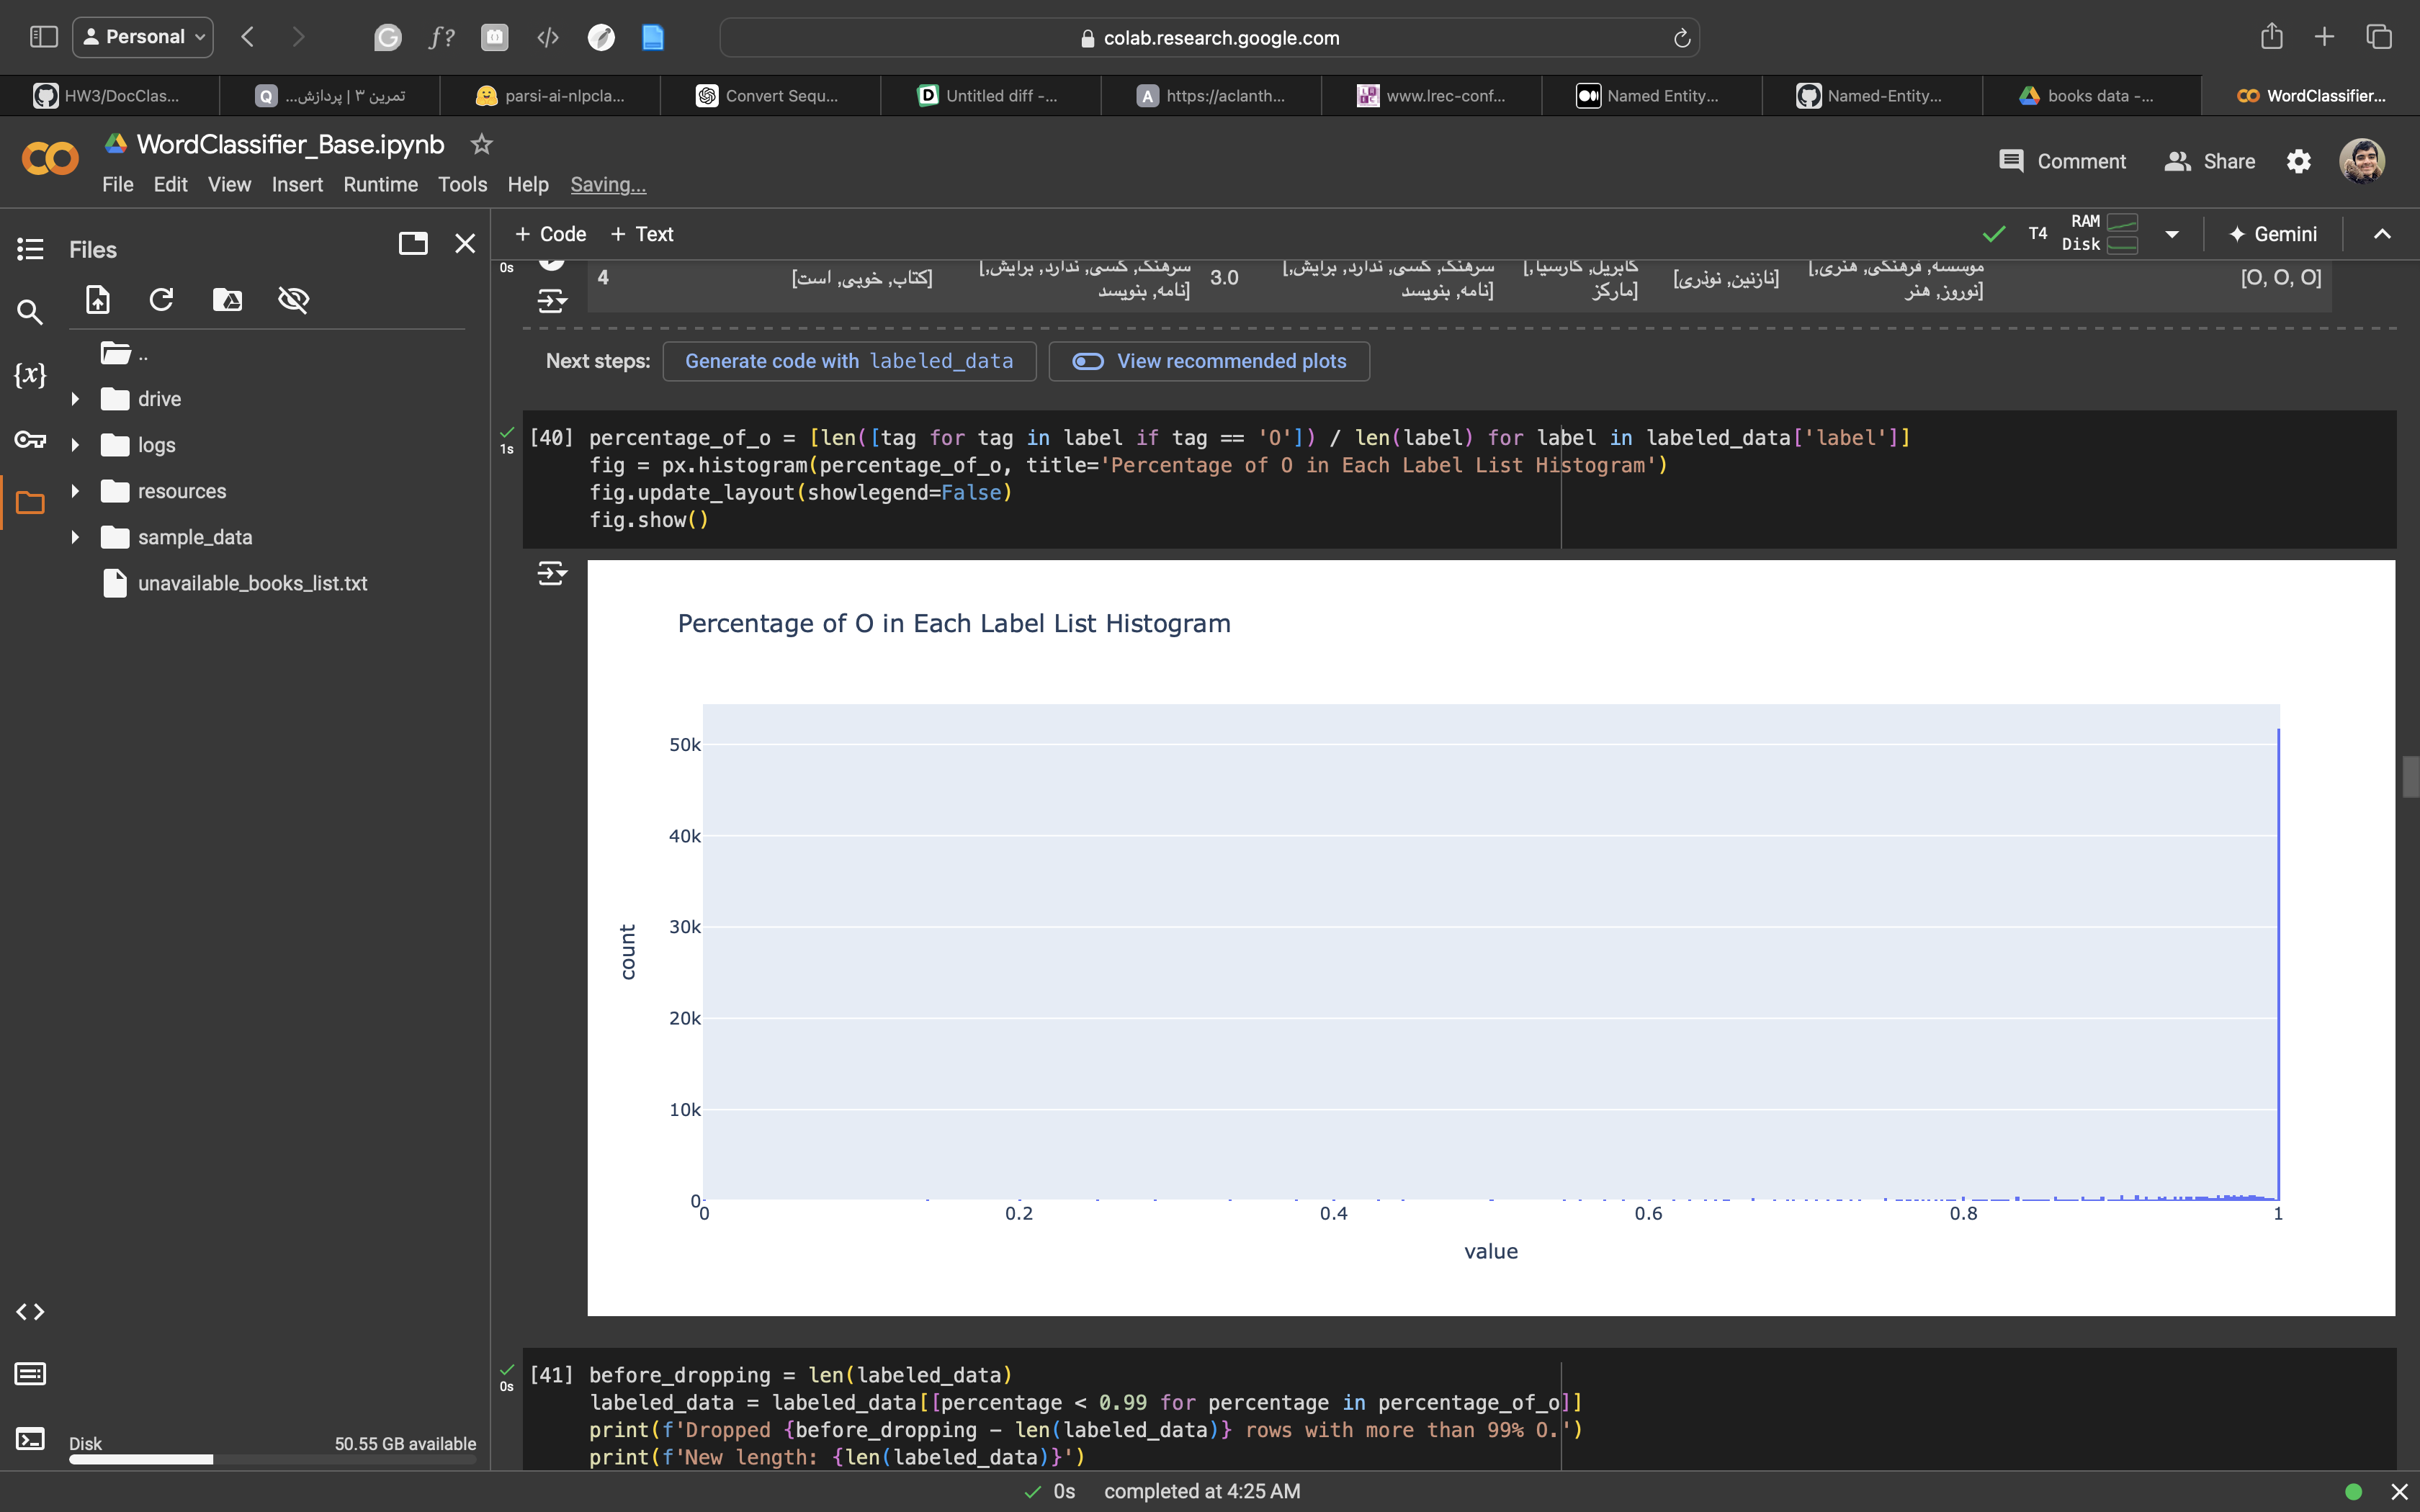
\includegraphics[width=0.5\textwidth]{img/1/1.png}
\end{figure}

\begin{figure}[h!]
    \caption{ Tag Distribution with O}
    \centering
    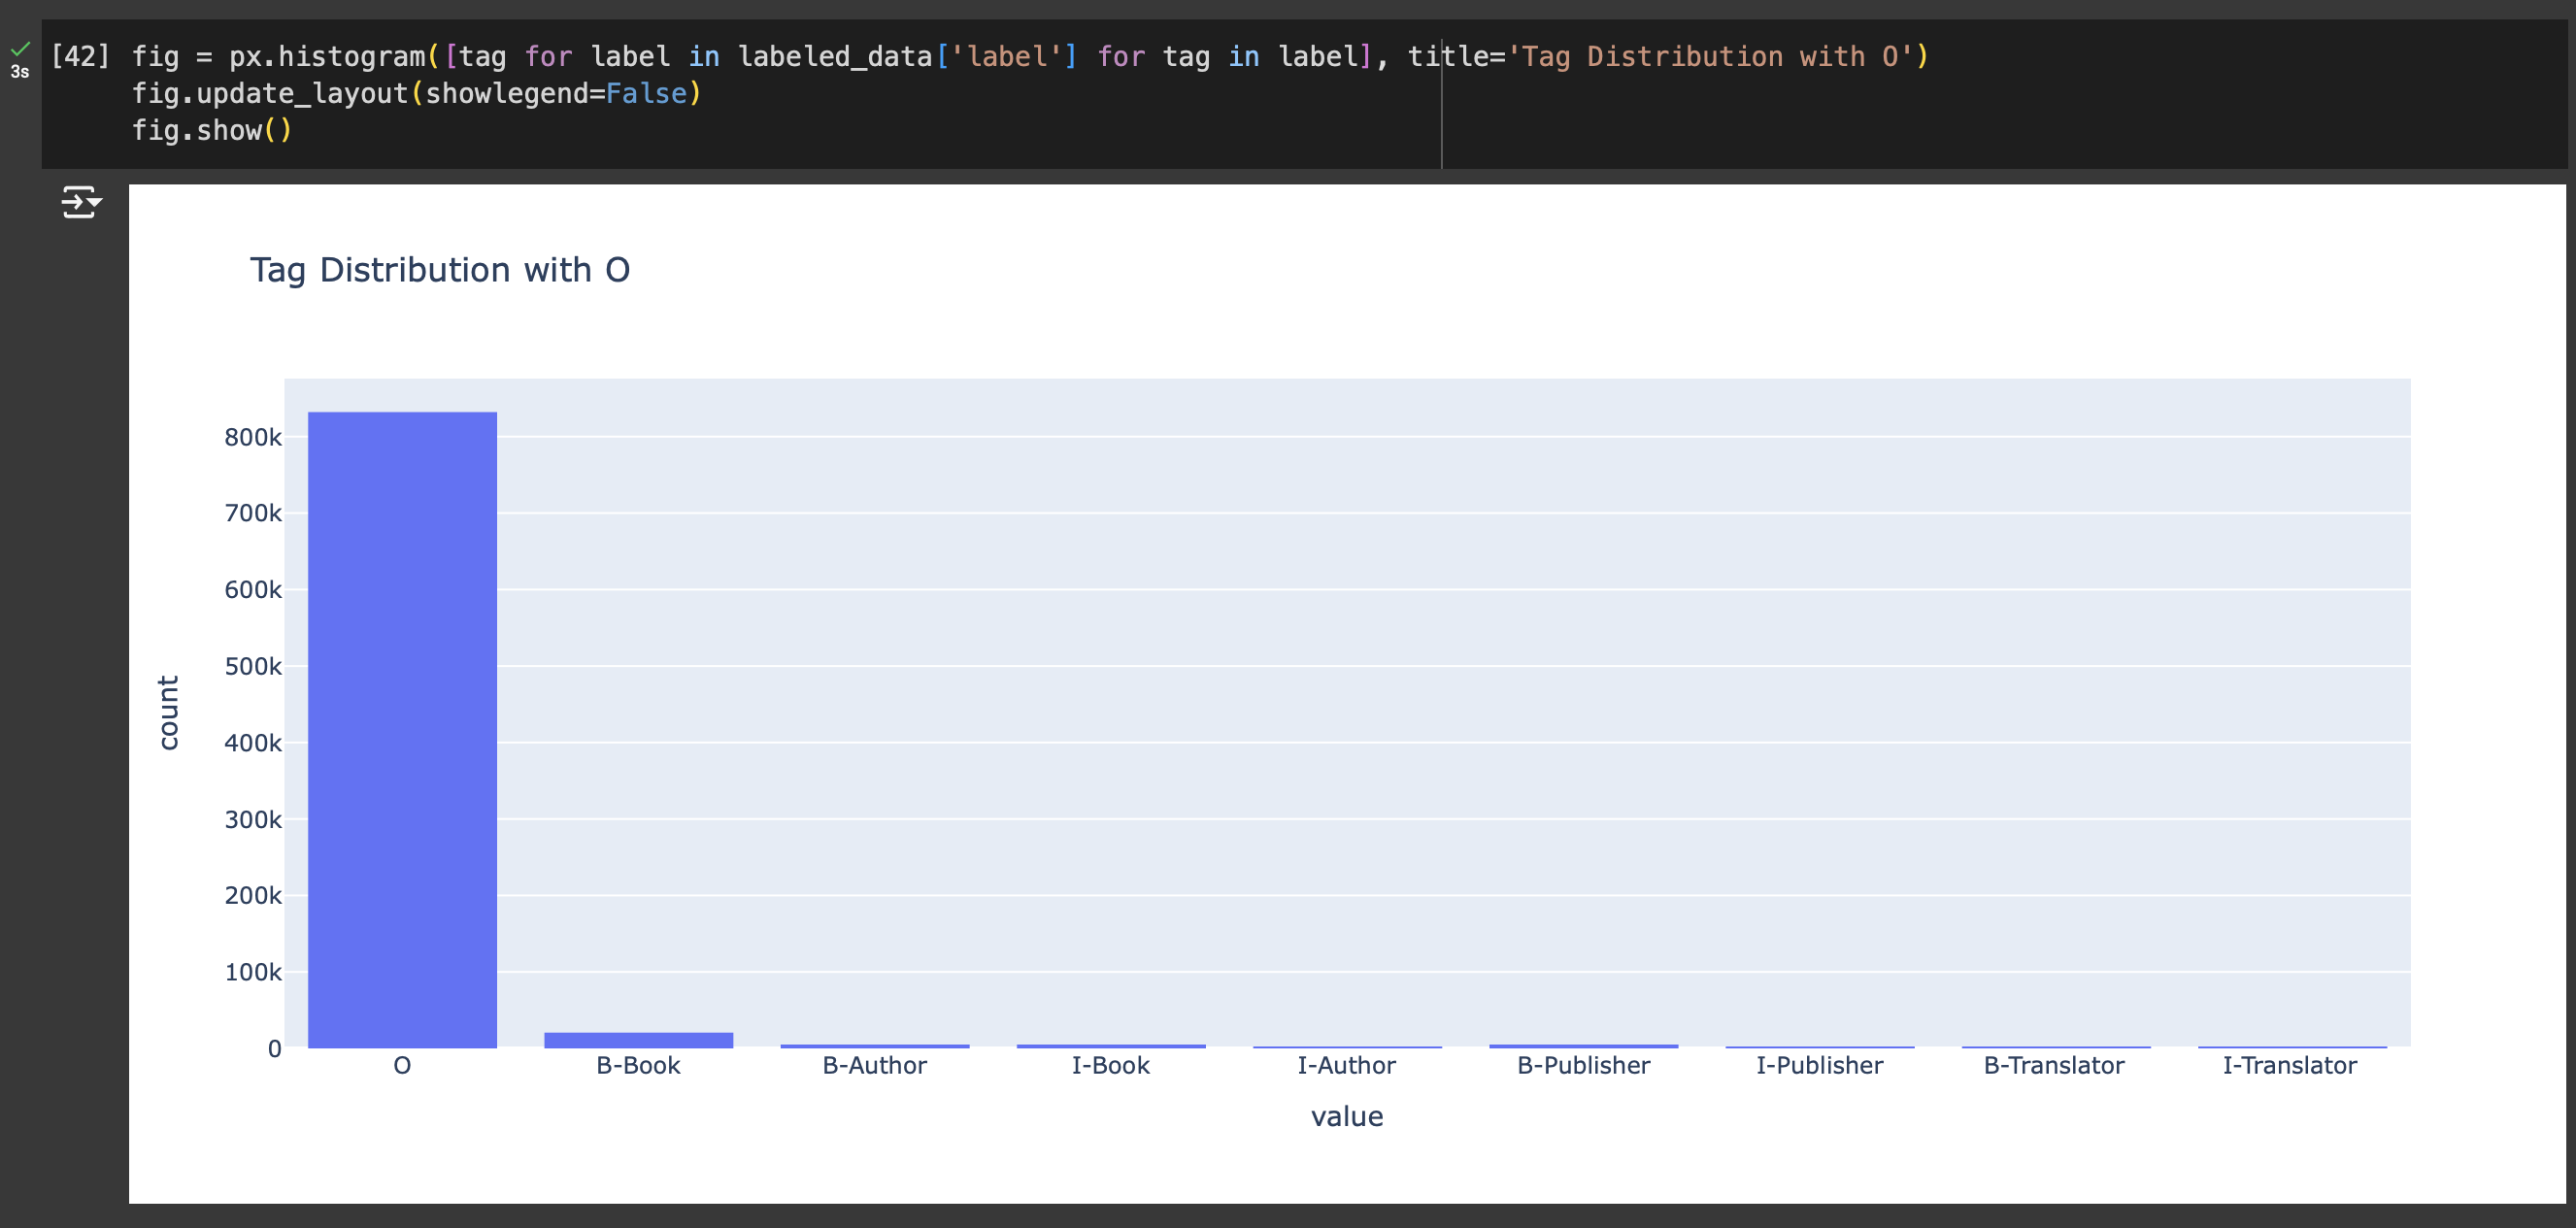
\includegraphics[width=0.5\textwidth]{img/1/2.png}
\end{figure}


\begin{figure}[h!]
    \caption{Tag distribution without O}
    \centering
    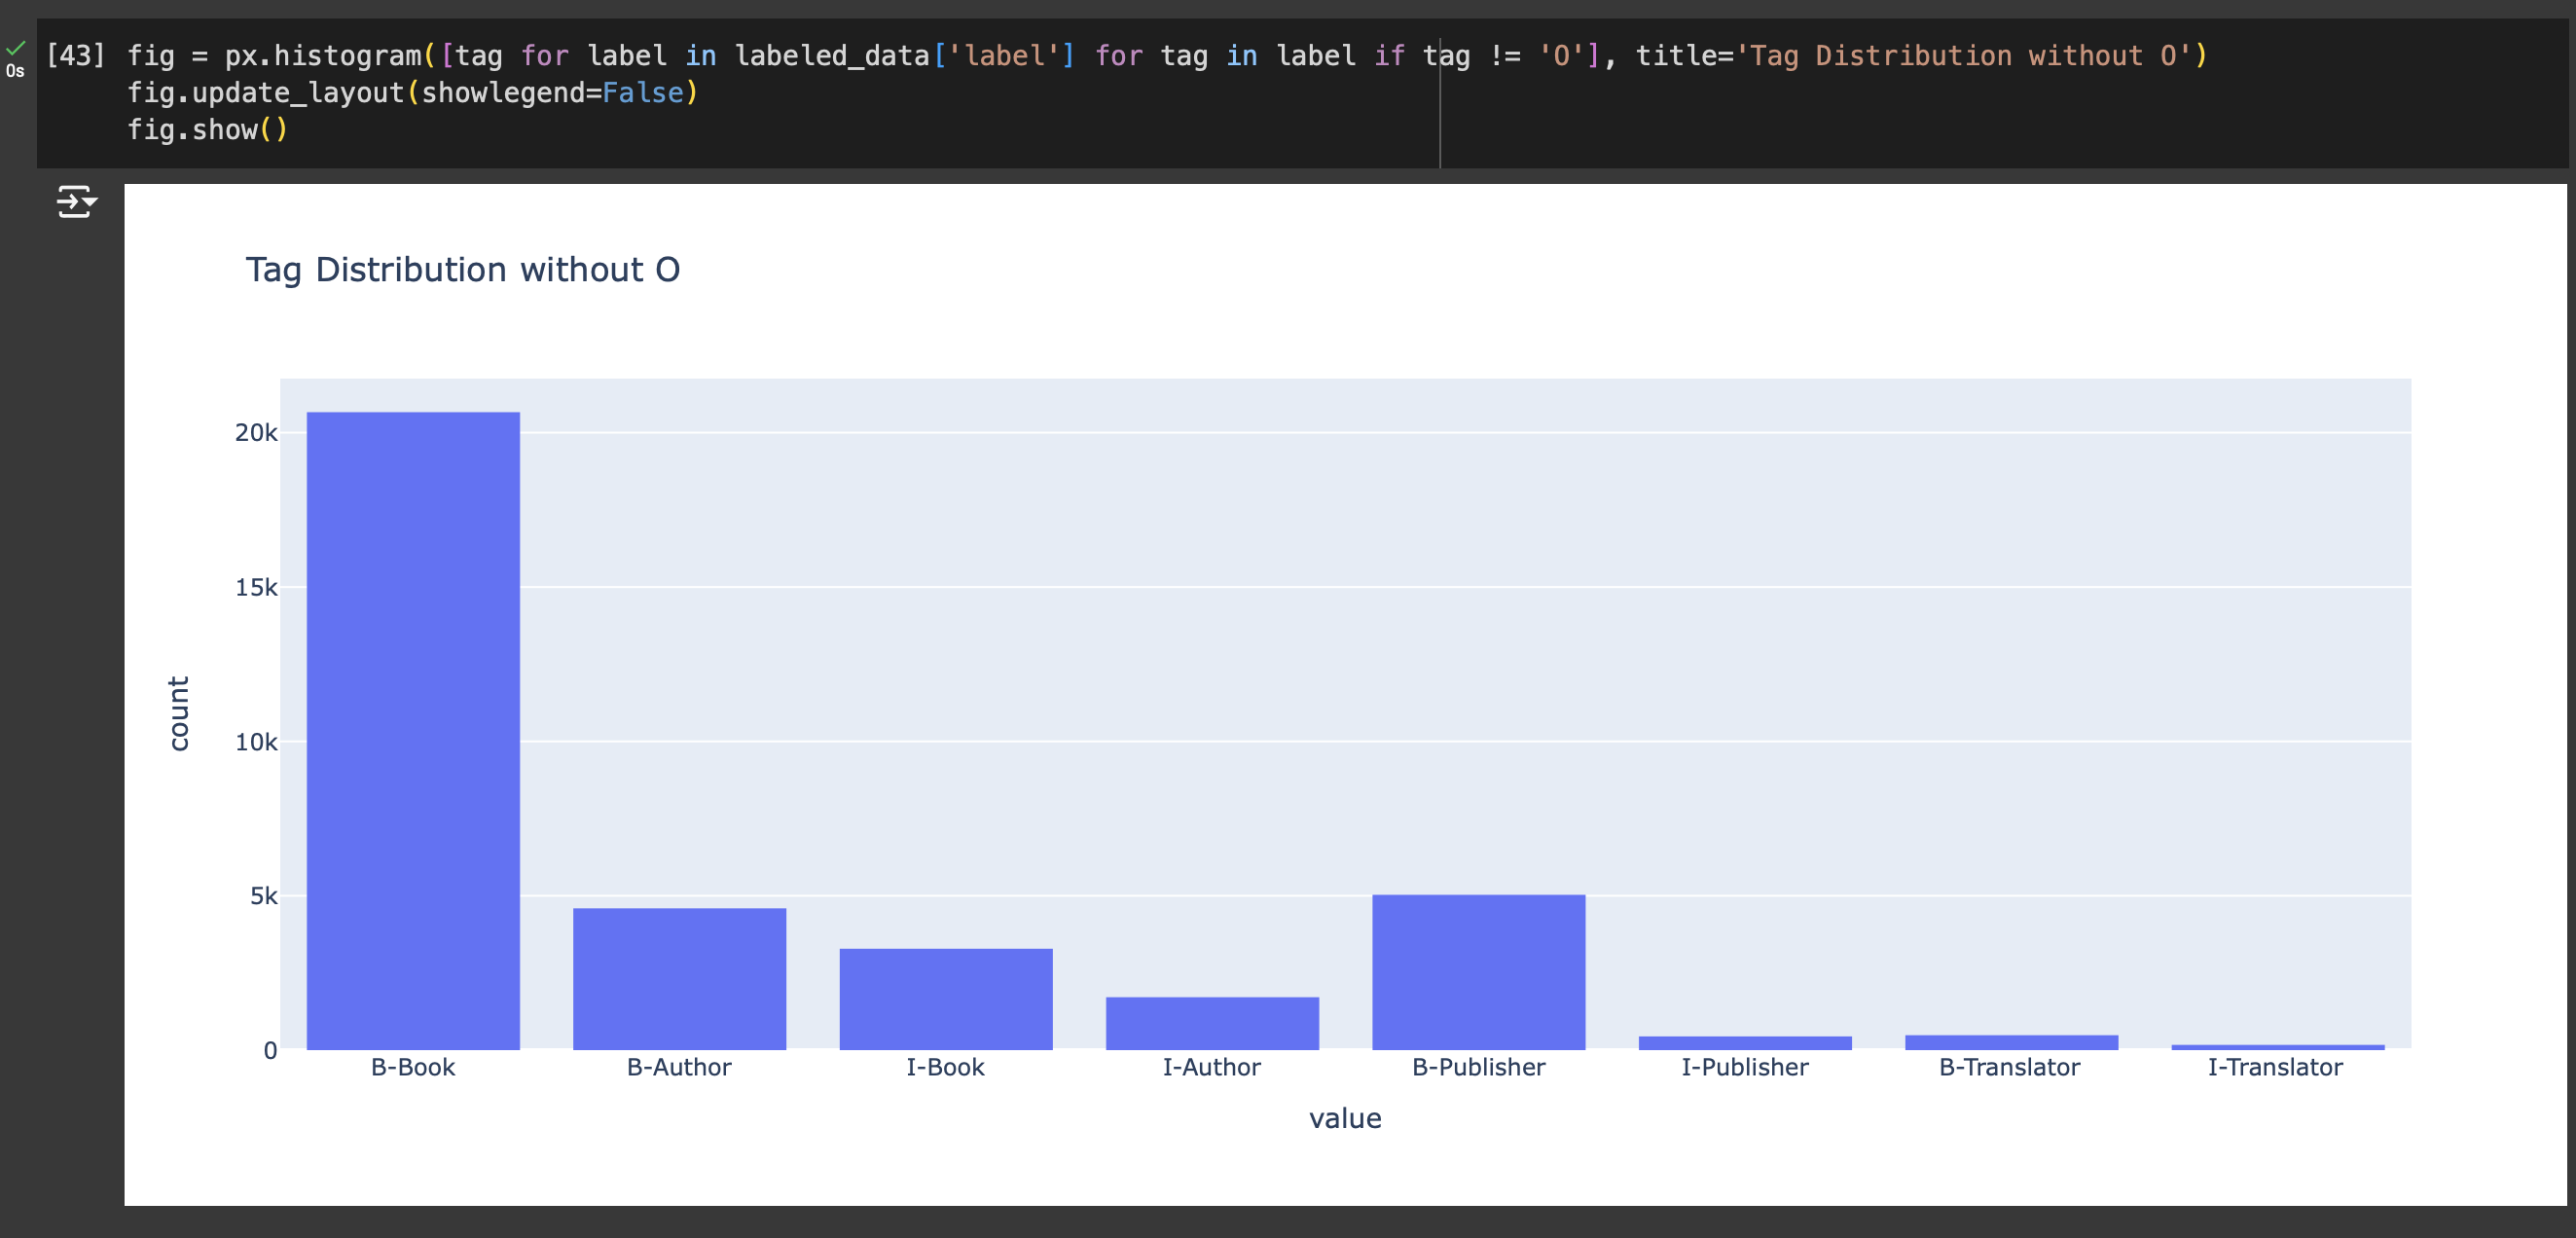
\includegraphics[width=0.5\textwidth]{img/1/3.png}
\end{figure}

\begin{figure}[h!]
    \caption{Sentence (Comment) Length Histogram}
    \centering
    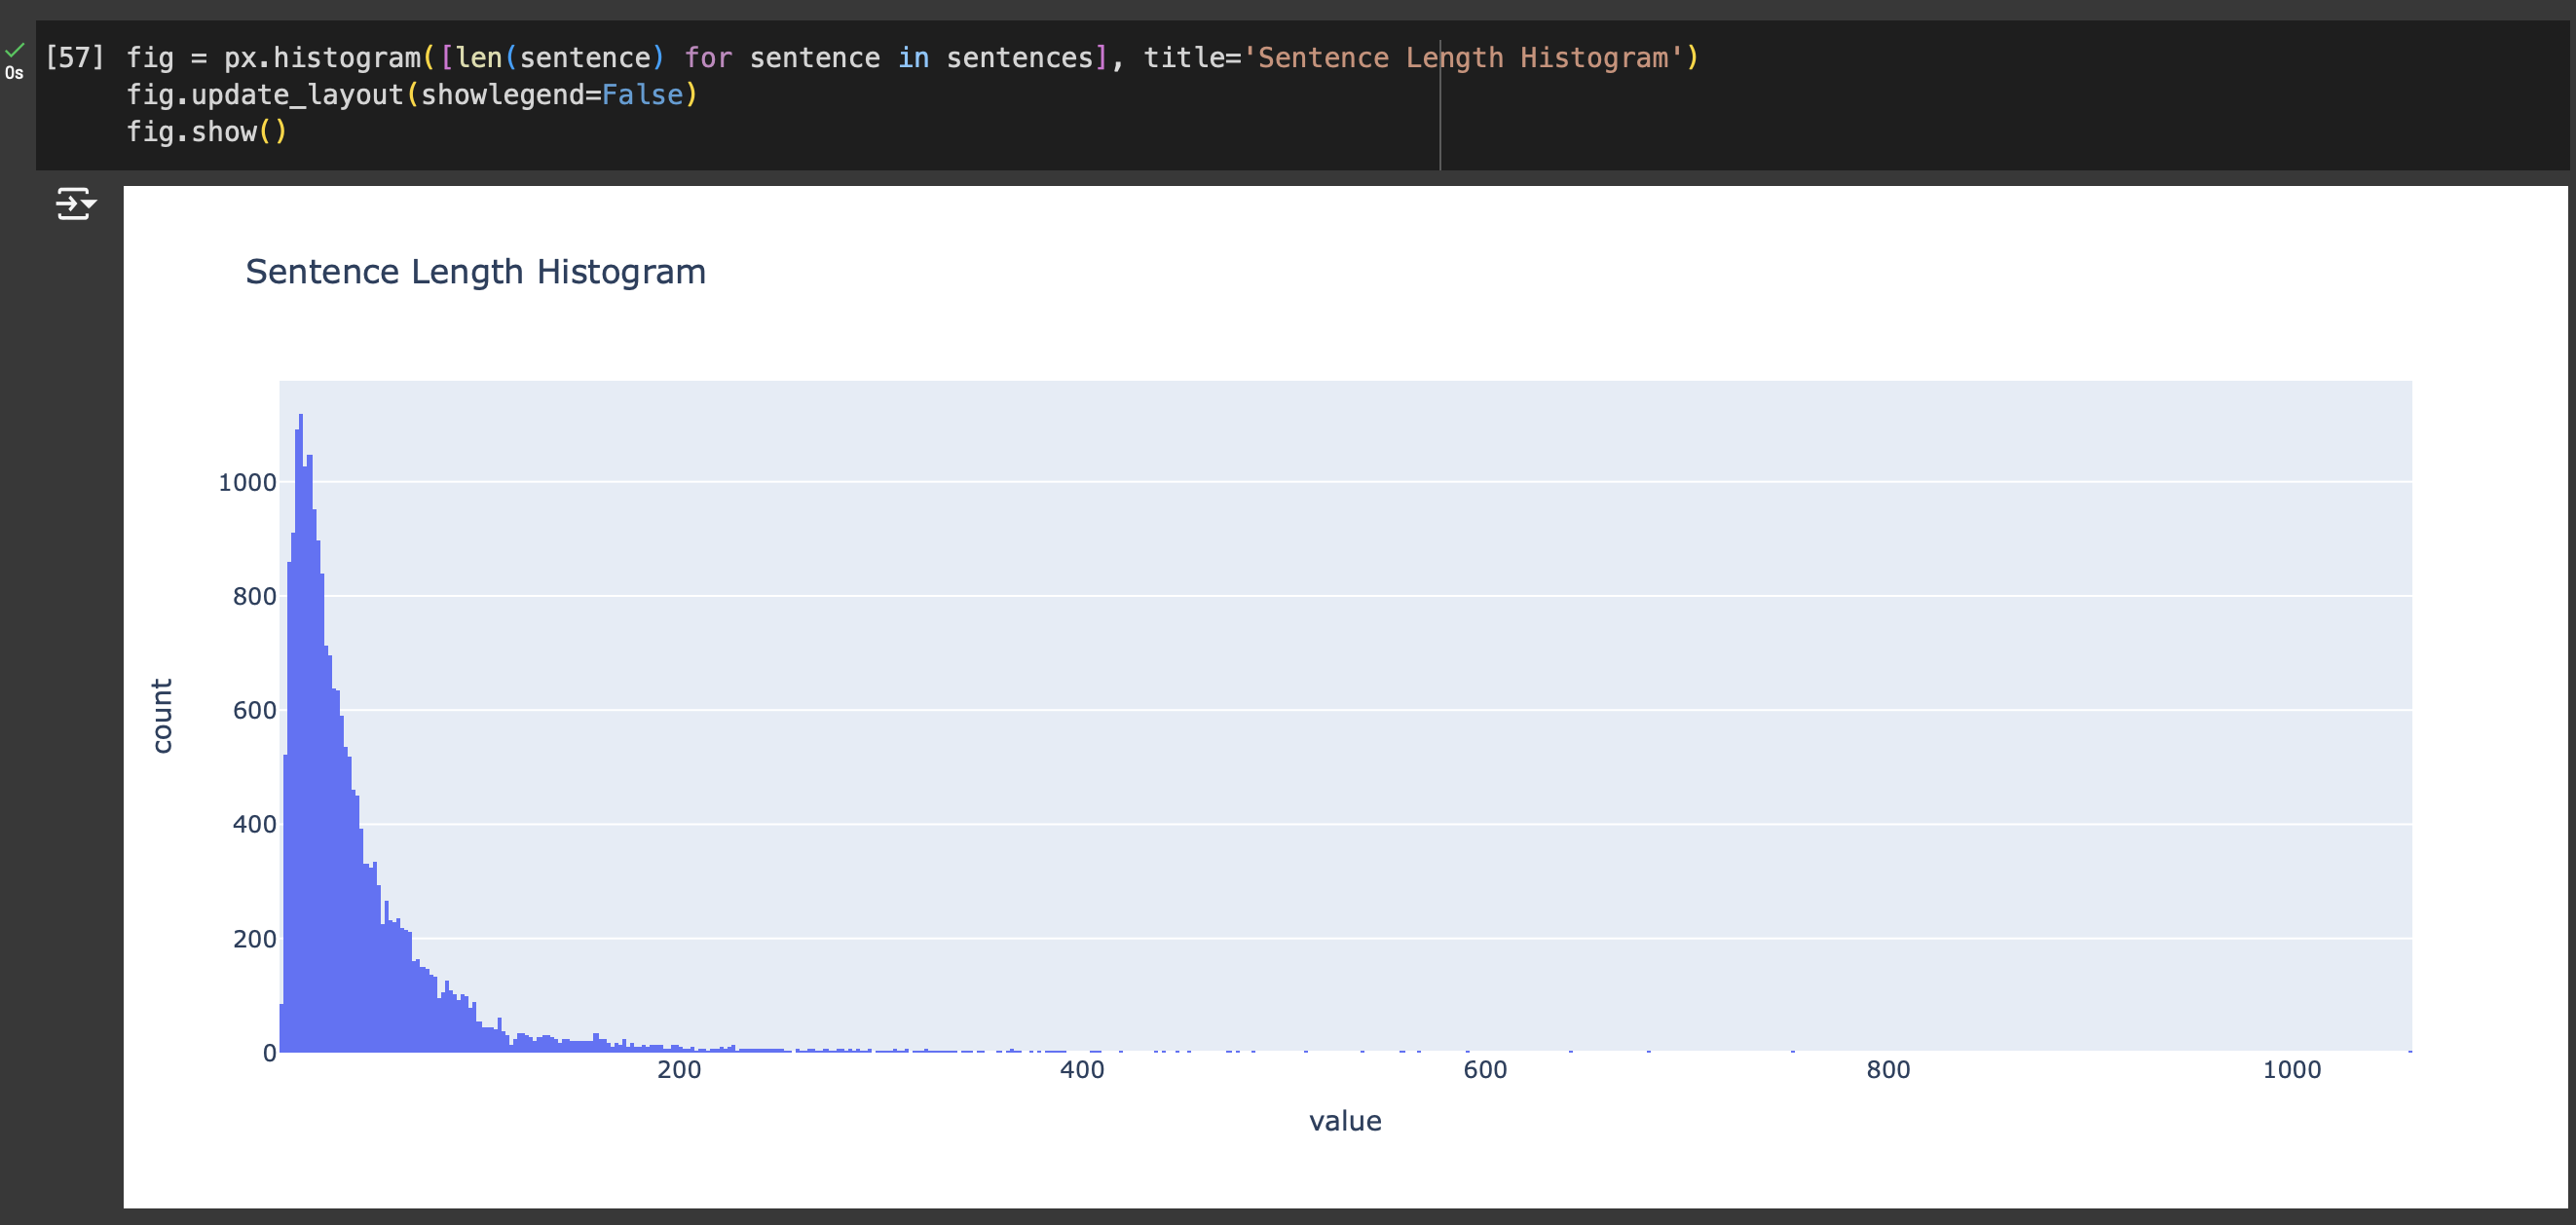
\includegraphics[width=0.5\textwidth]{img/1/4.png}
\end{figure}

\begin{figure}[h!]
    \caption{LSTM Model}
    \centering
    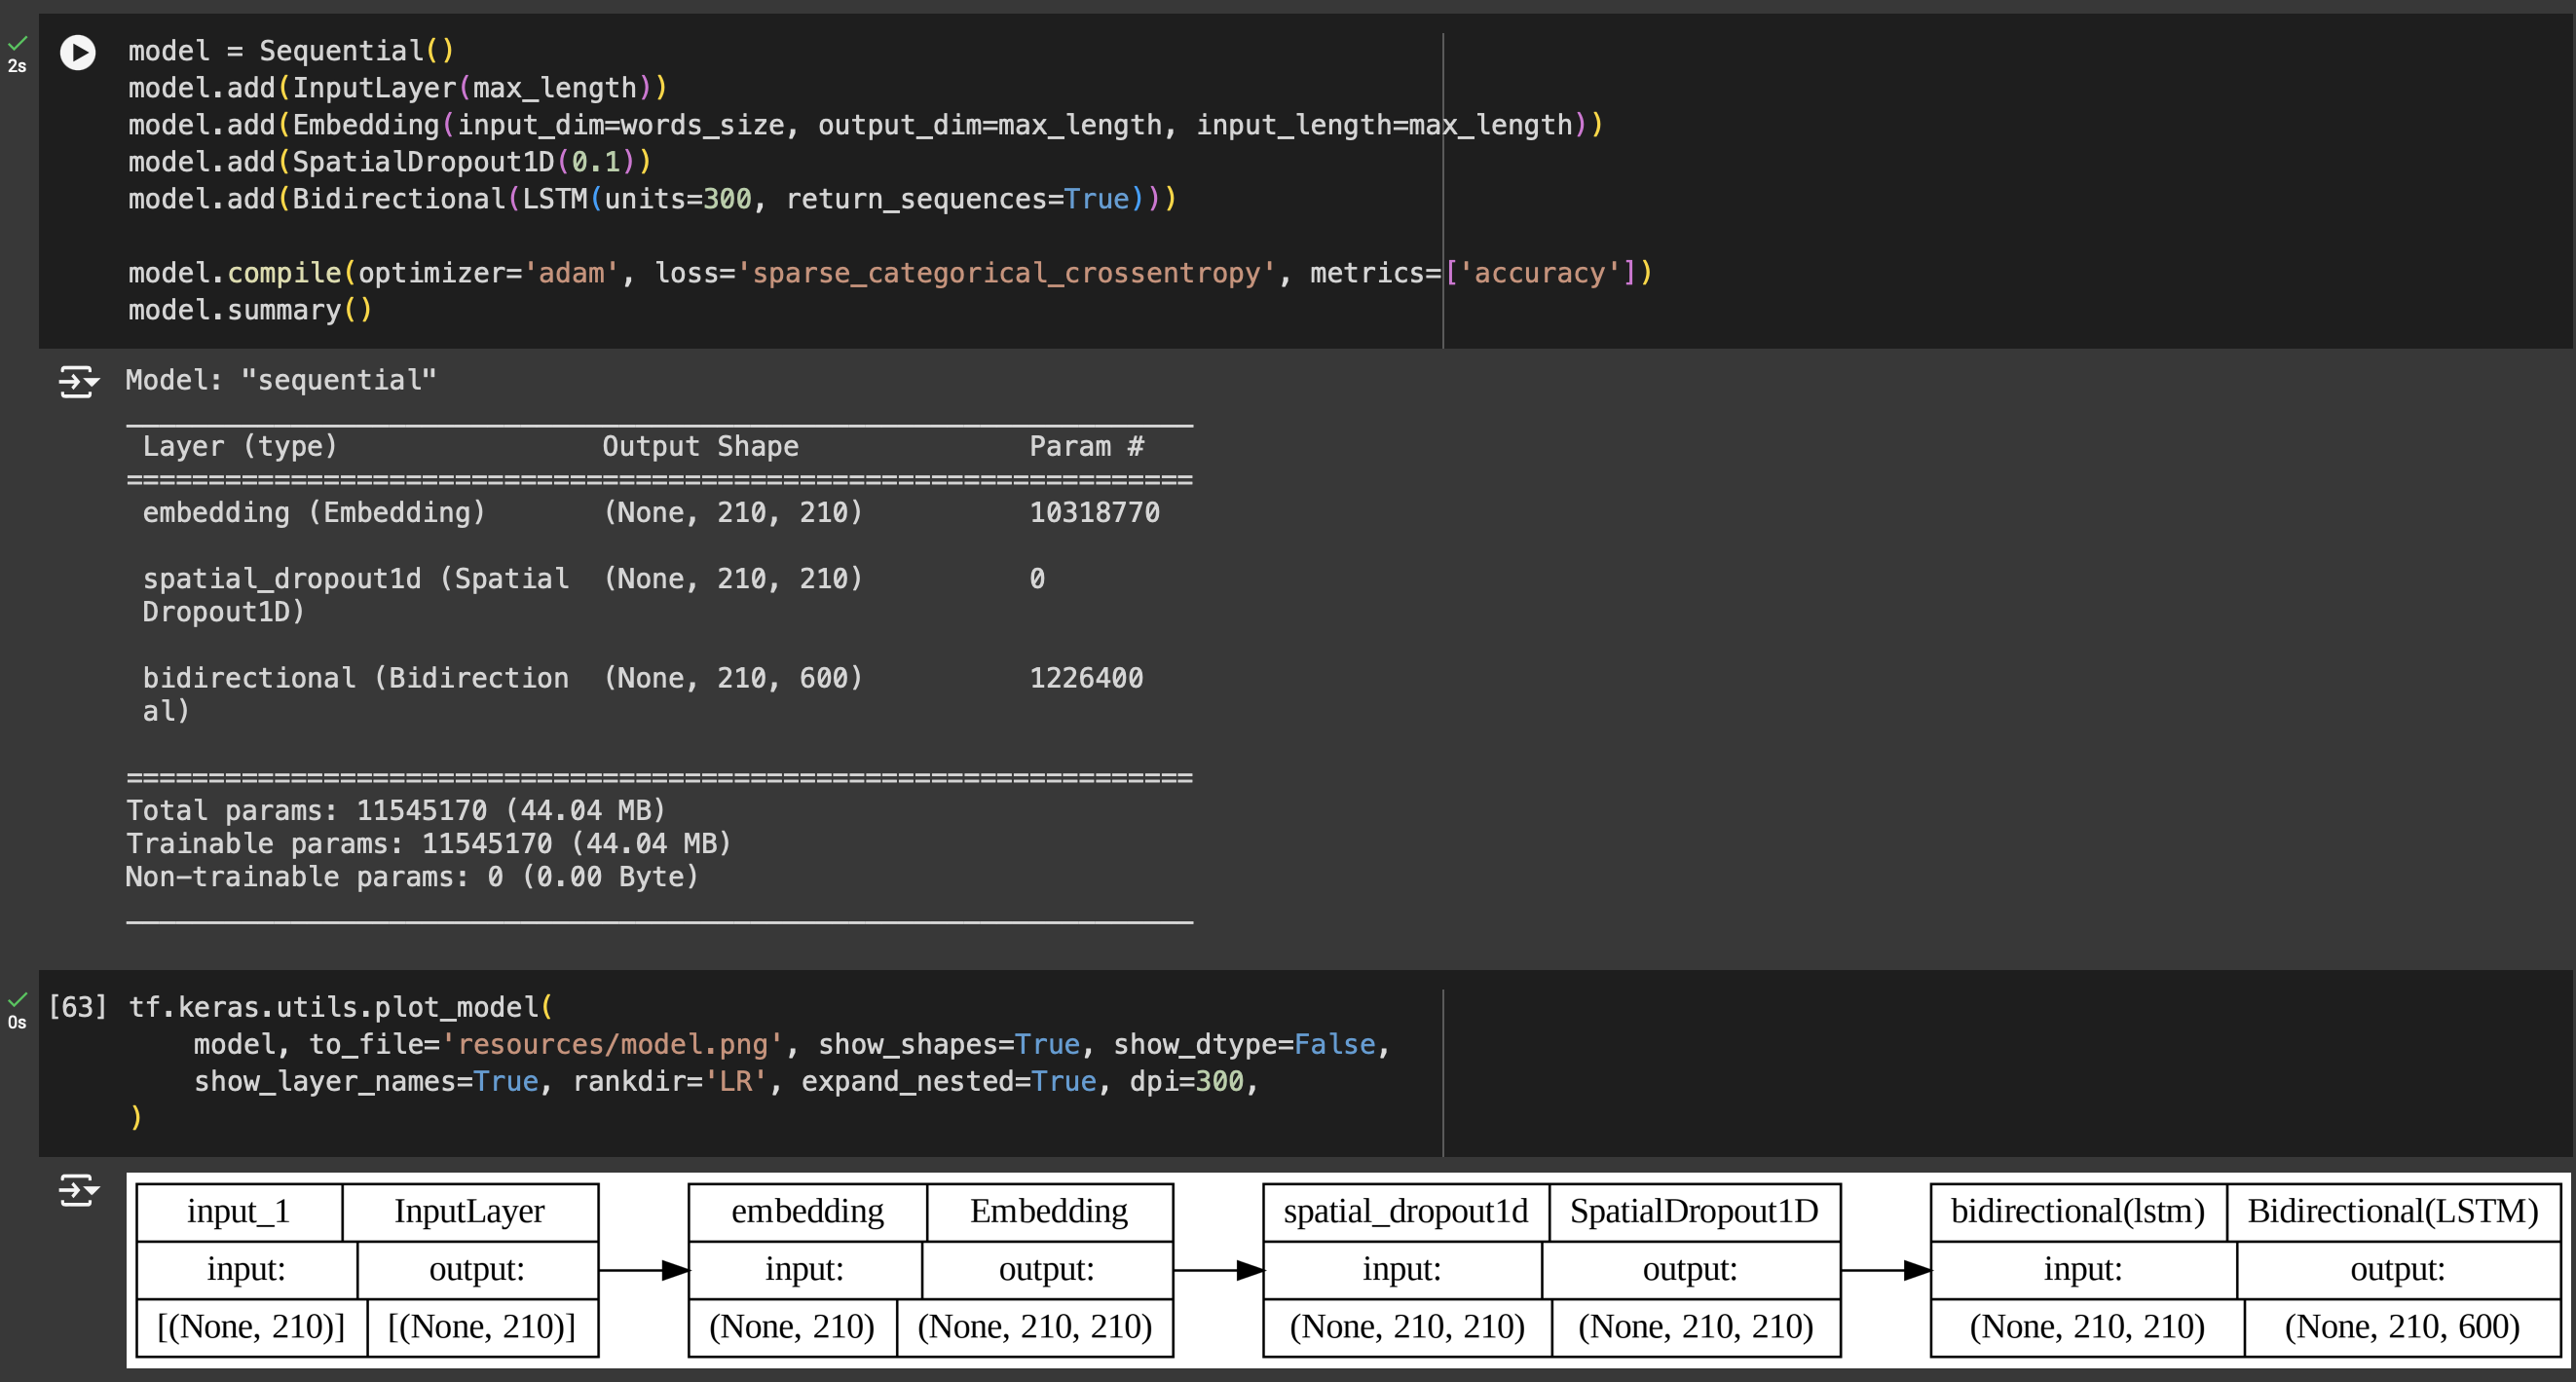
\includegraphics[width=0.5\textwidth]{img/1/5.png}
\end{figure}

\begin{figure}[h!]
    \caption{Accuracy and Loss During Training}
    \centering
    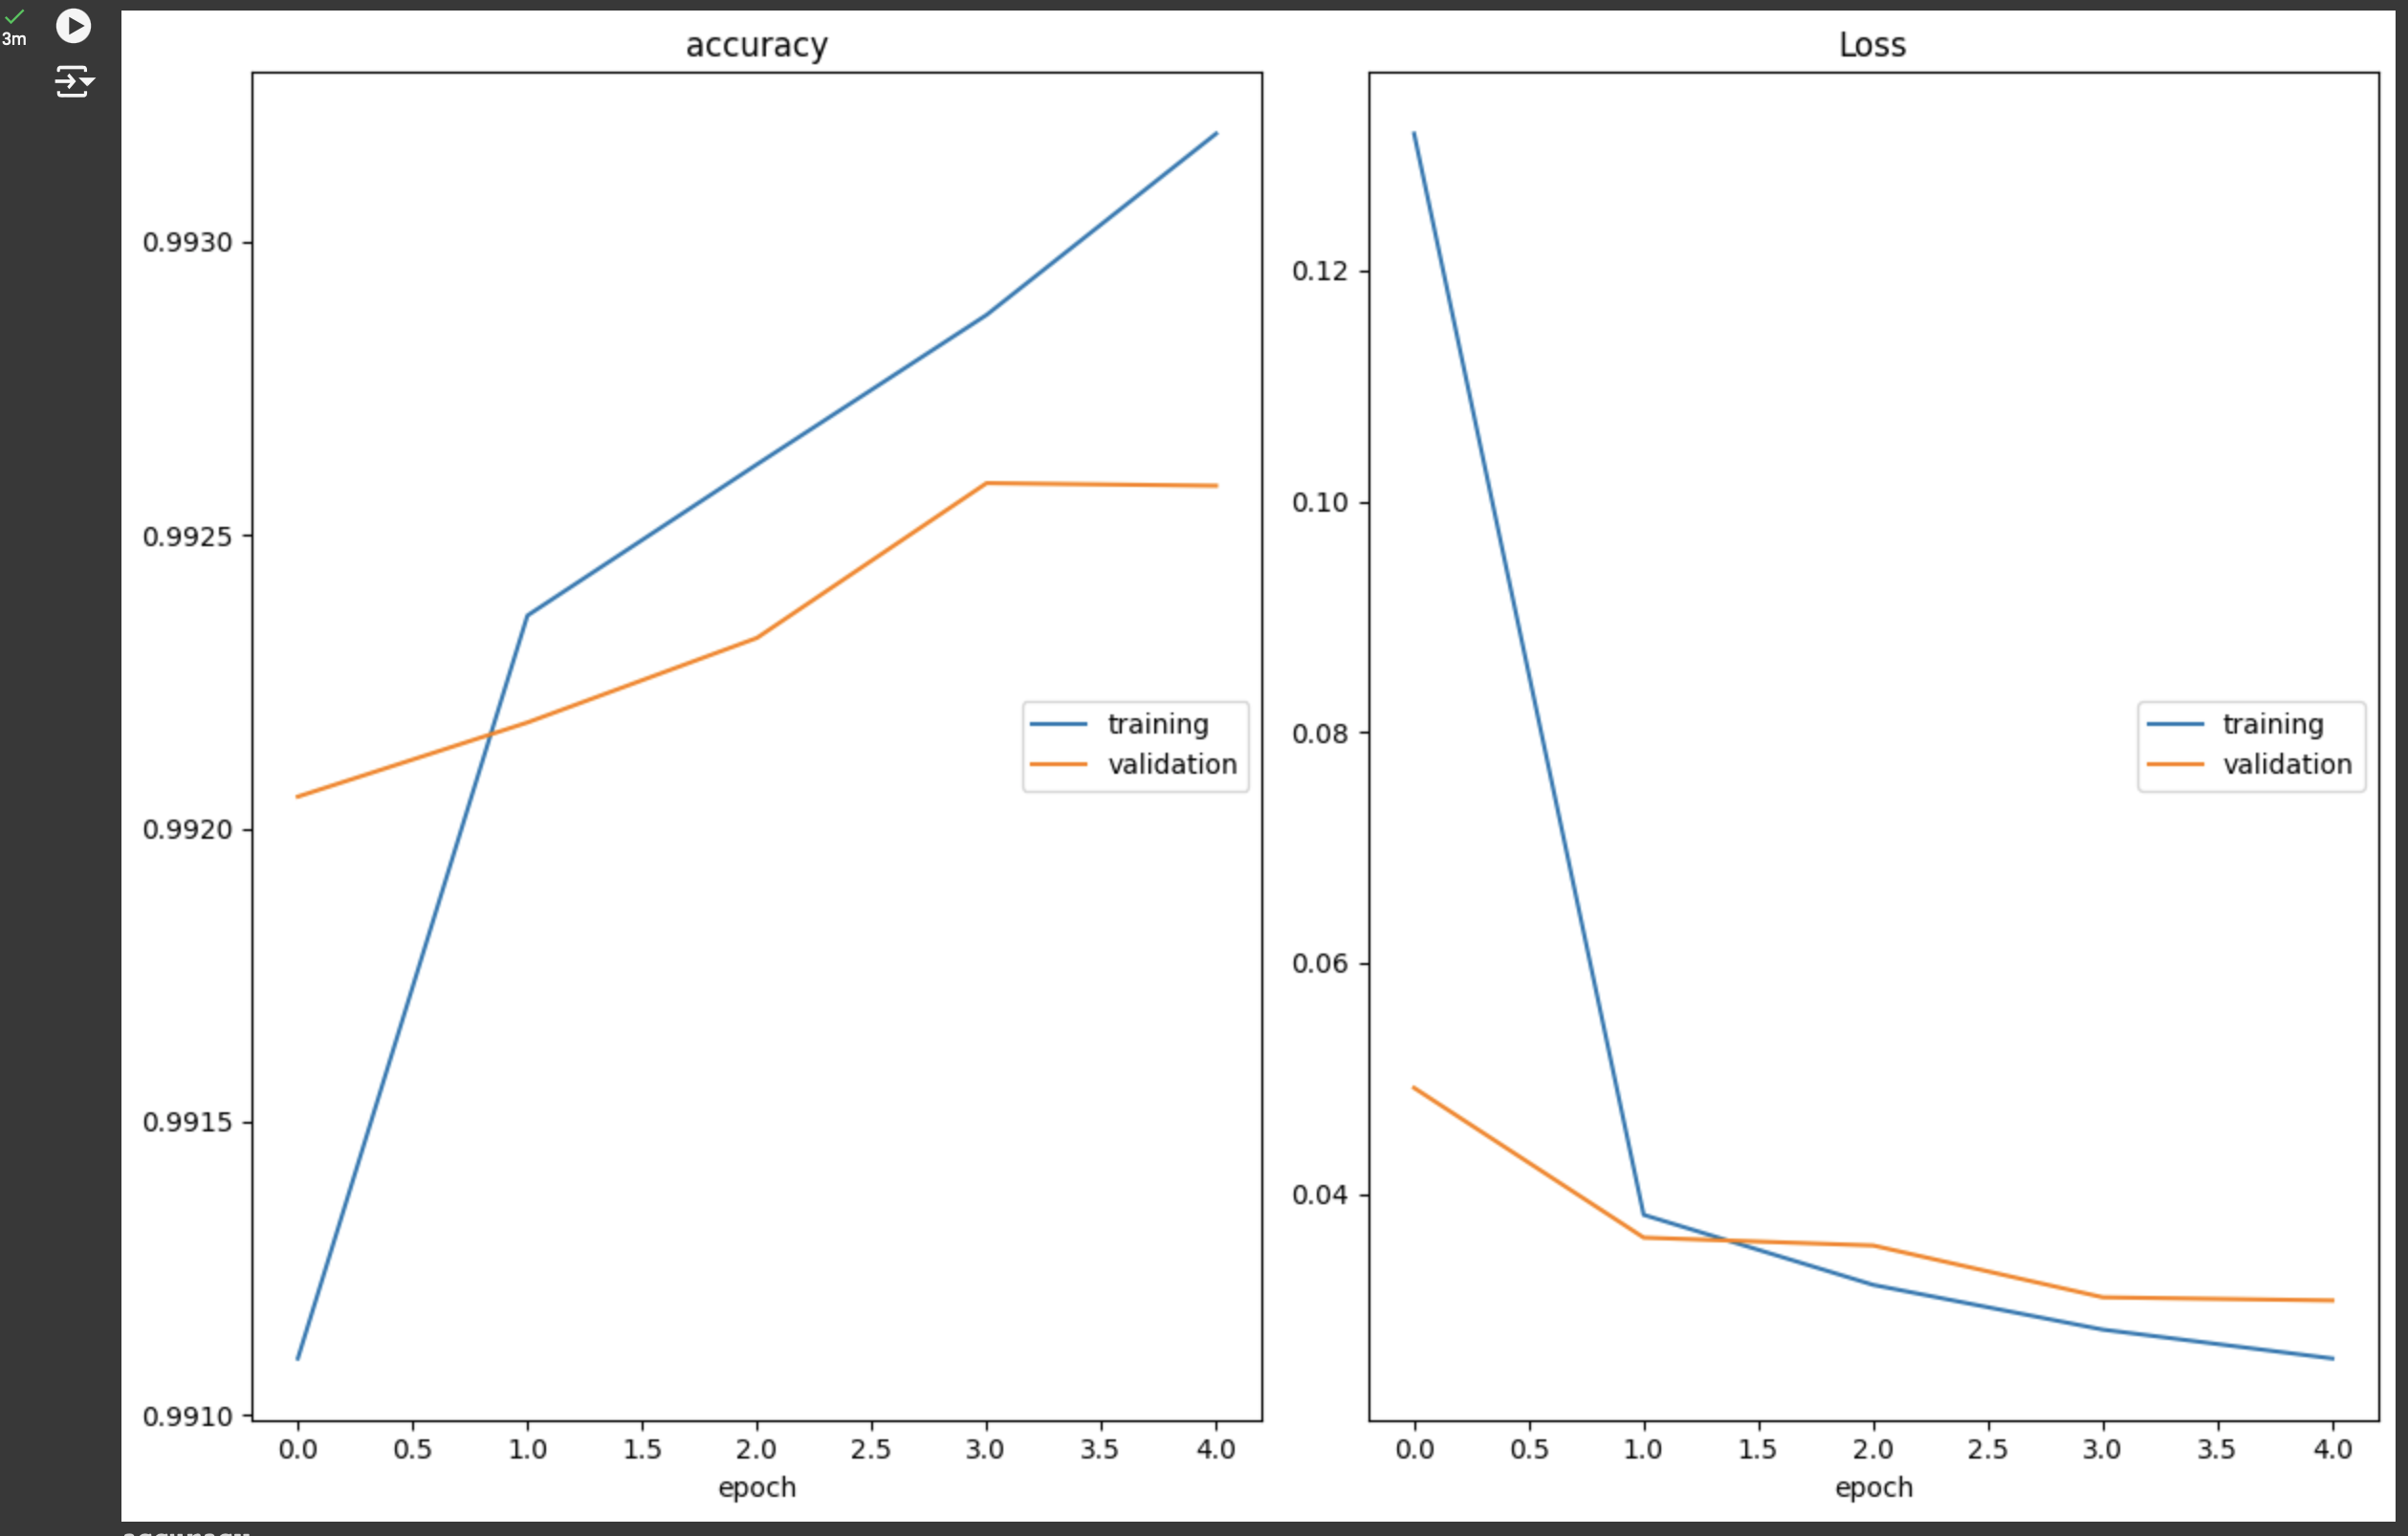
\includegraphics[width=0.5\textwidth]{img/1/6.png}
\end{figure}

\begin{figure}[h!]
    \caption{Text of Running the Model}
    \centering
    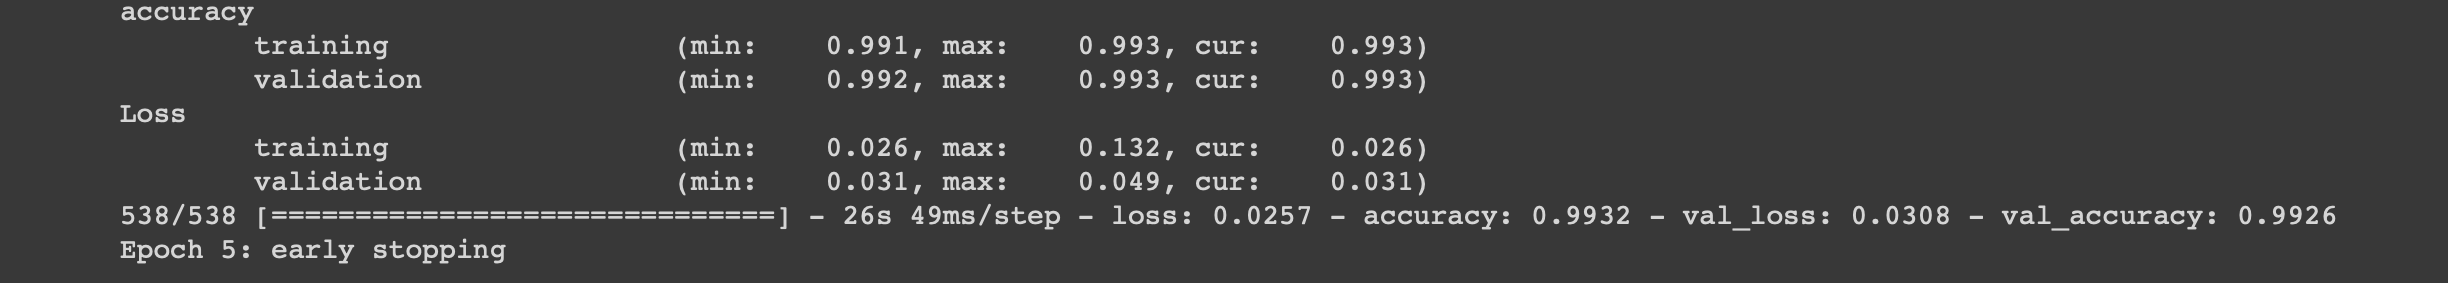
\includegraphics[width=0.5\textwidth]{img/1/7.png}
\end{figure}

\begin{figure}[h!]
    \caption{The Sentence in the Doc}
    \centering
    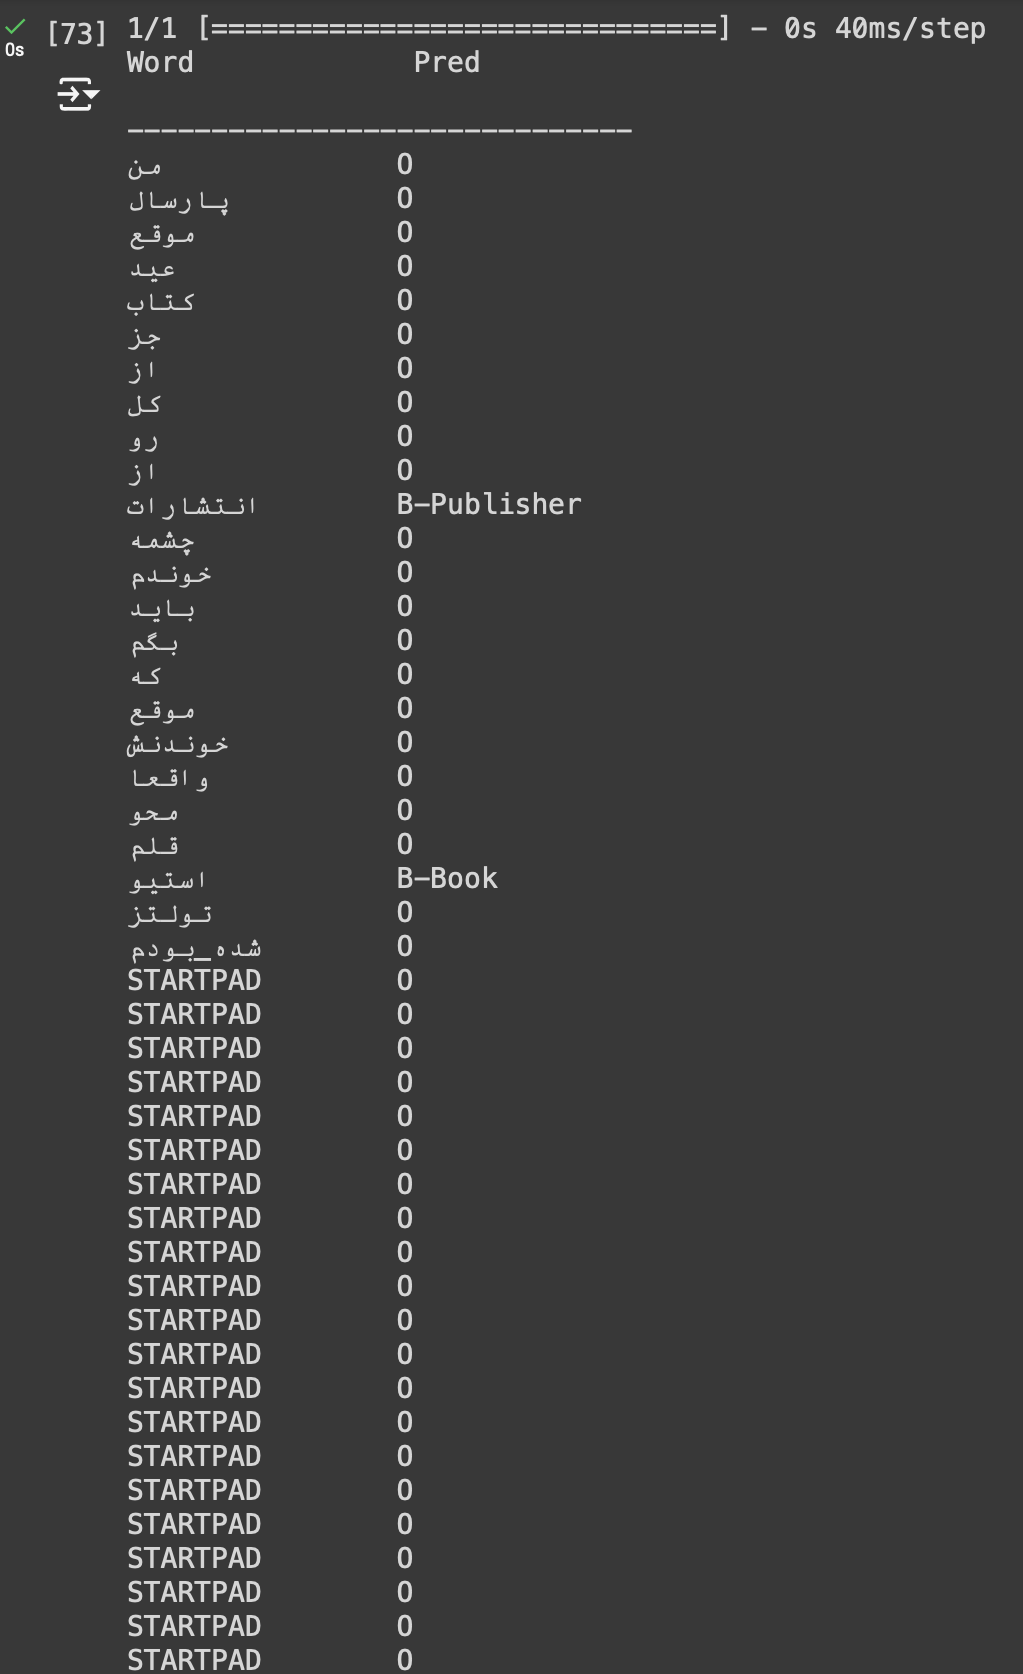
\includegraphics[width=0.5\textwidth]{img/1/8.png}
\end{figure}


\begin{figure}[h!]
    \caption{Classification Report}
    \centering
    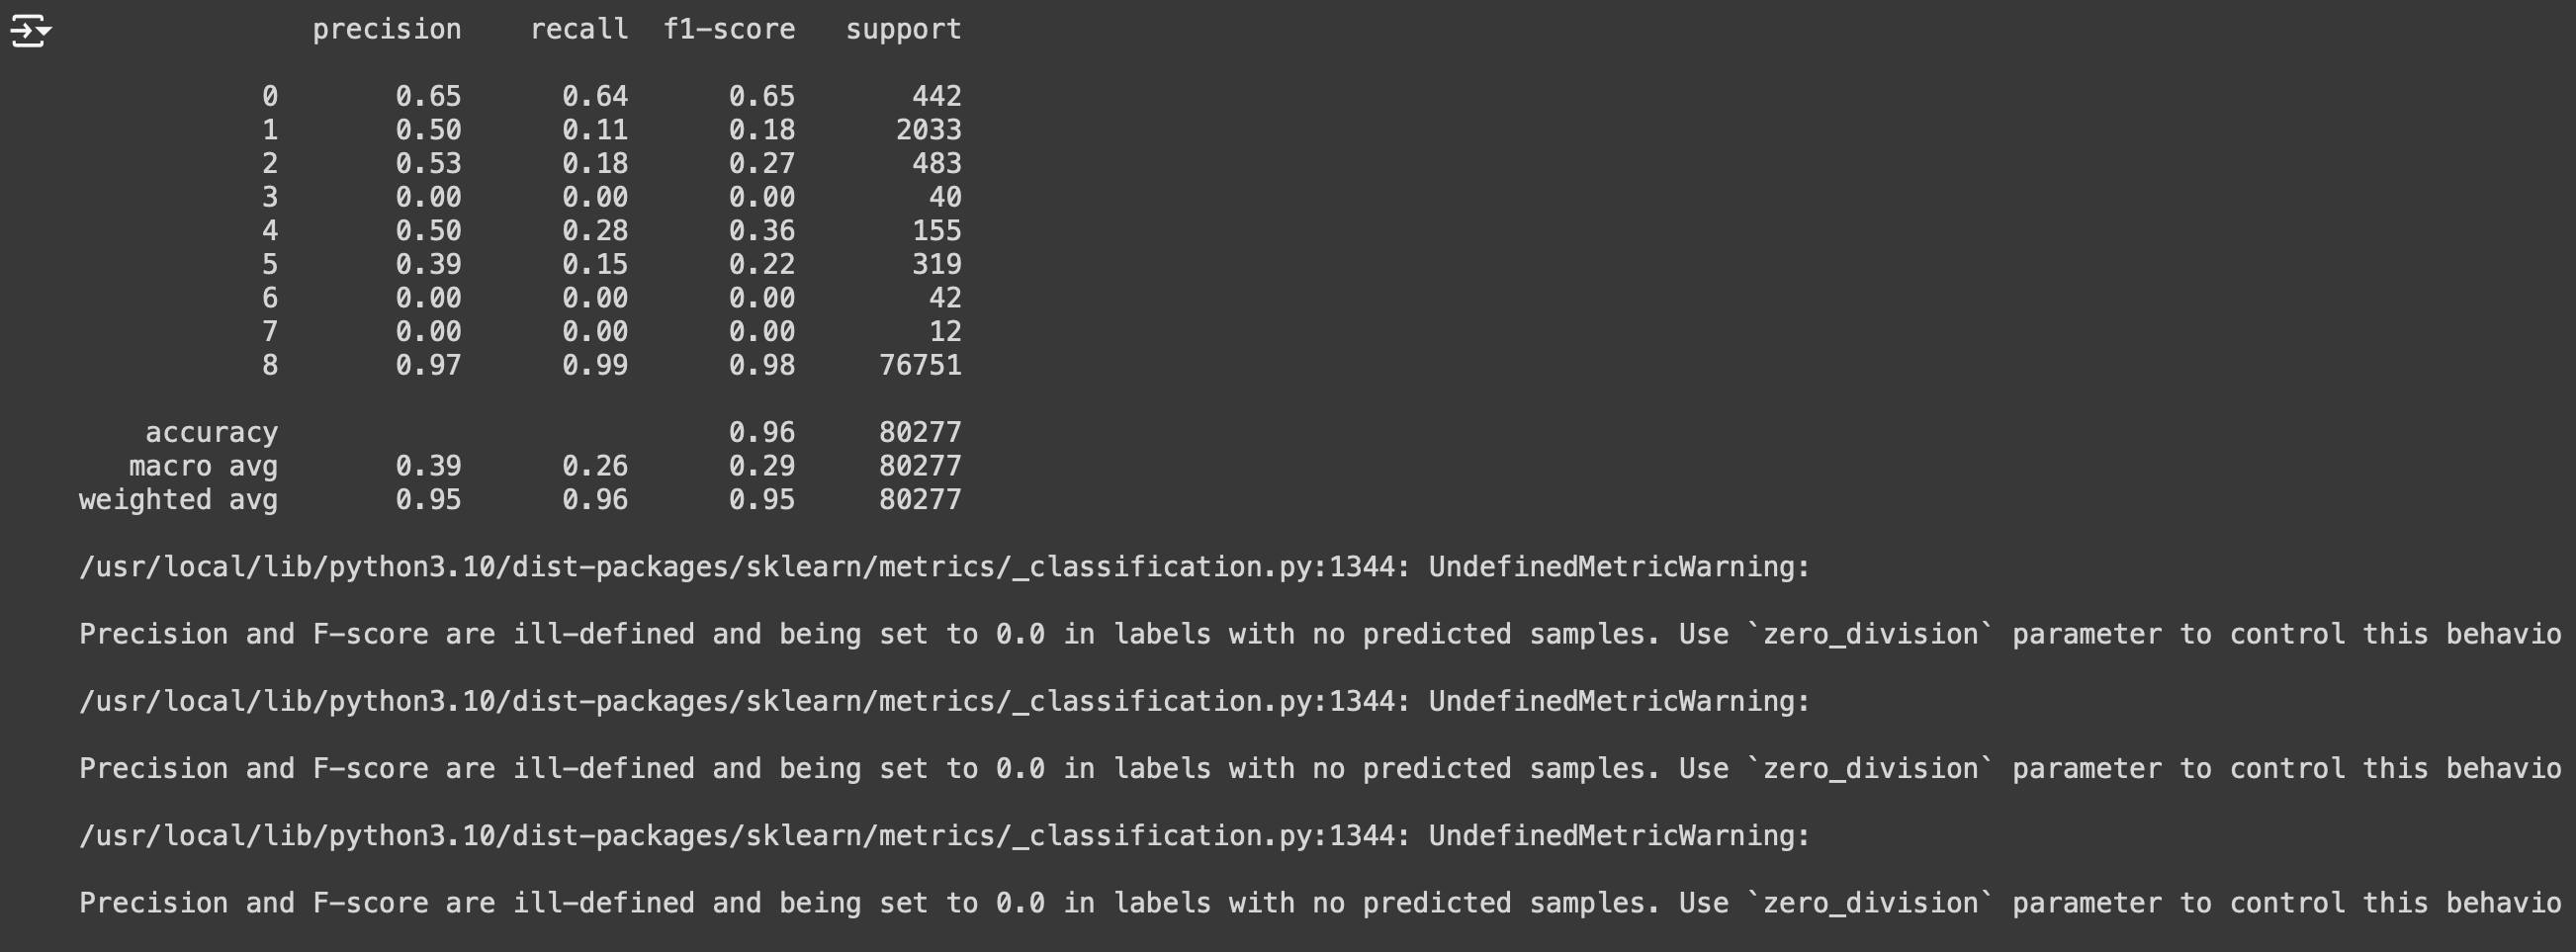
\includegraphics[width=0.5\textwidth]{img/1/10.png}
\end{figure}


\begin{figure}[h!]
    \caption{Confusion matrix}
    \centering
    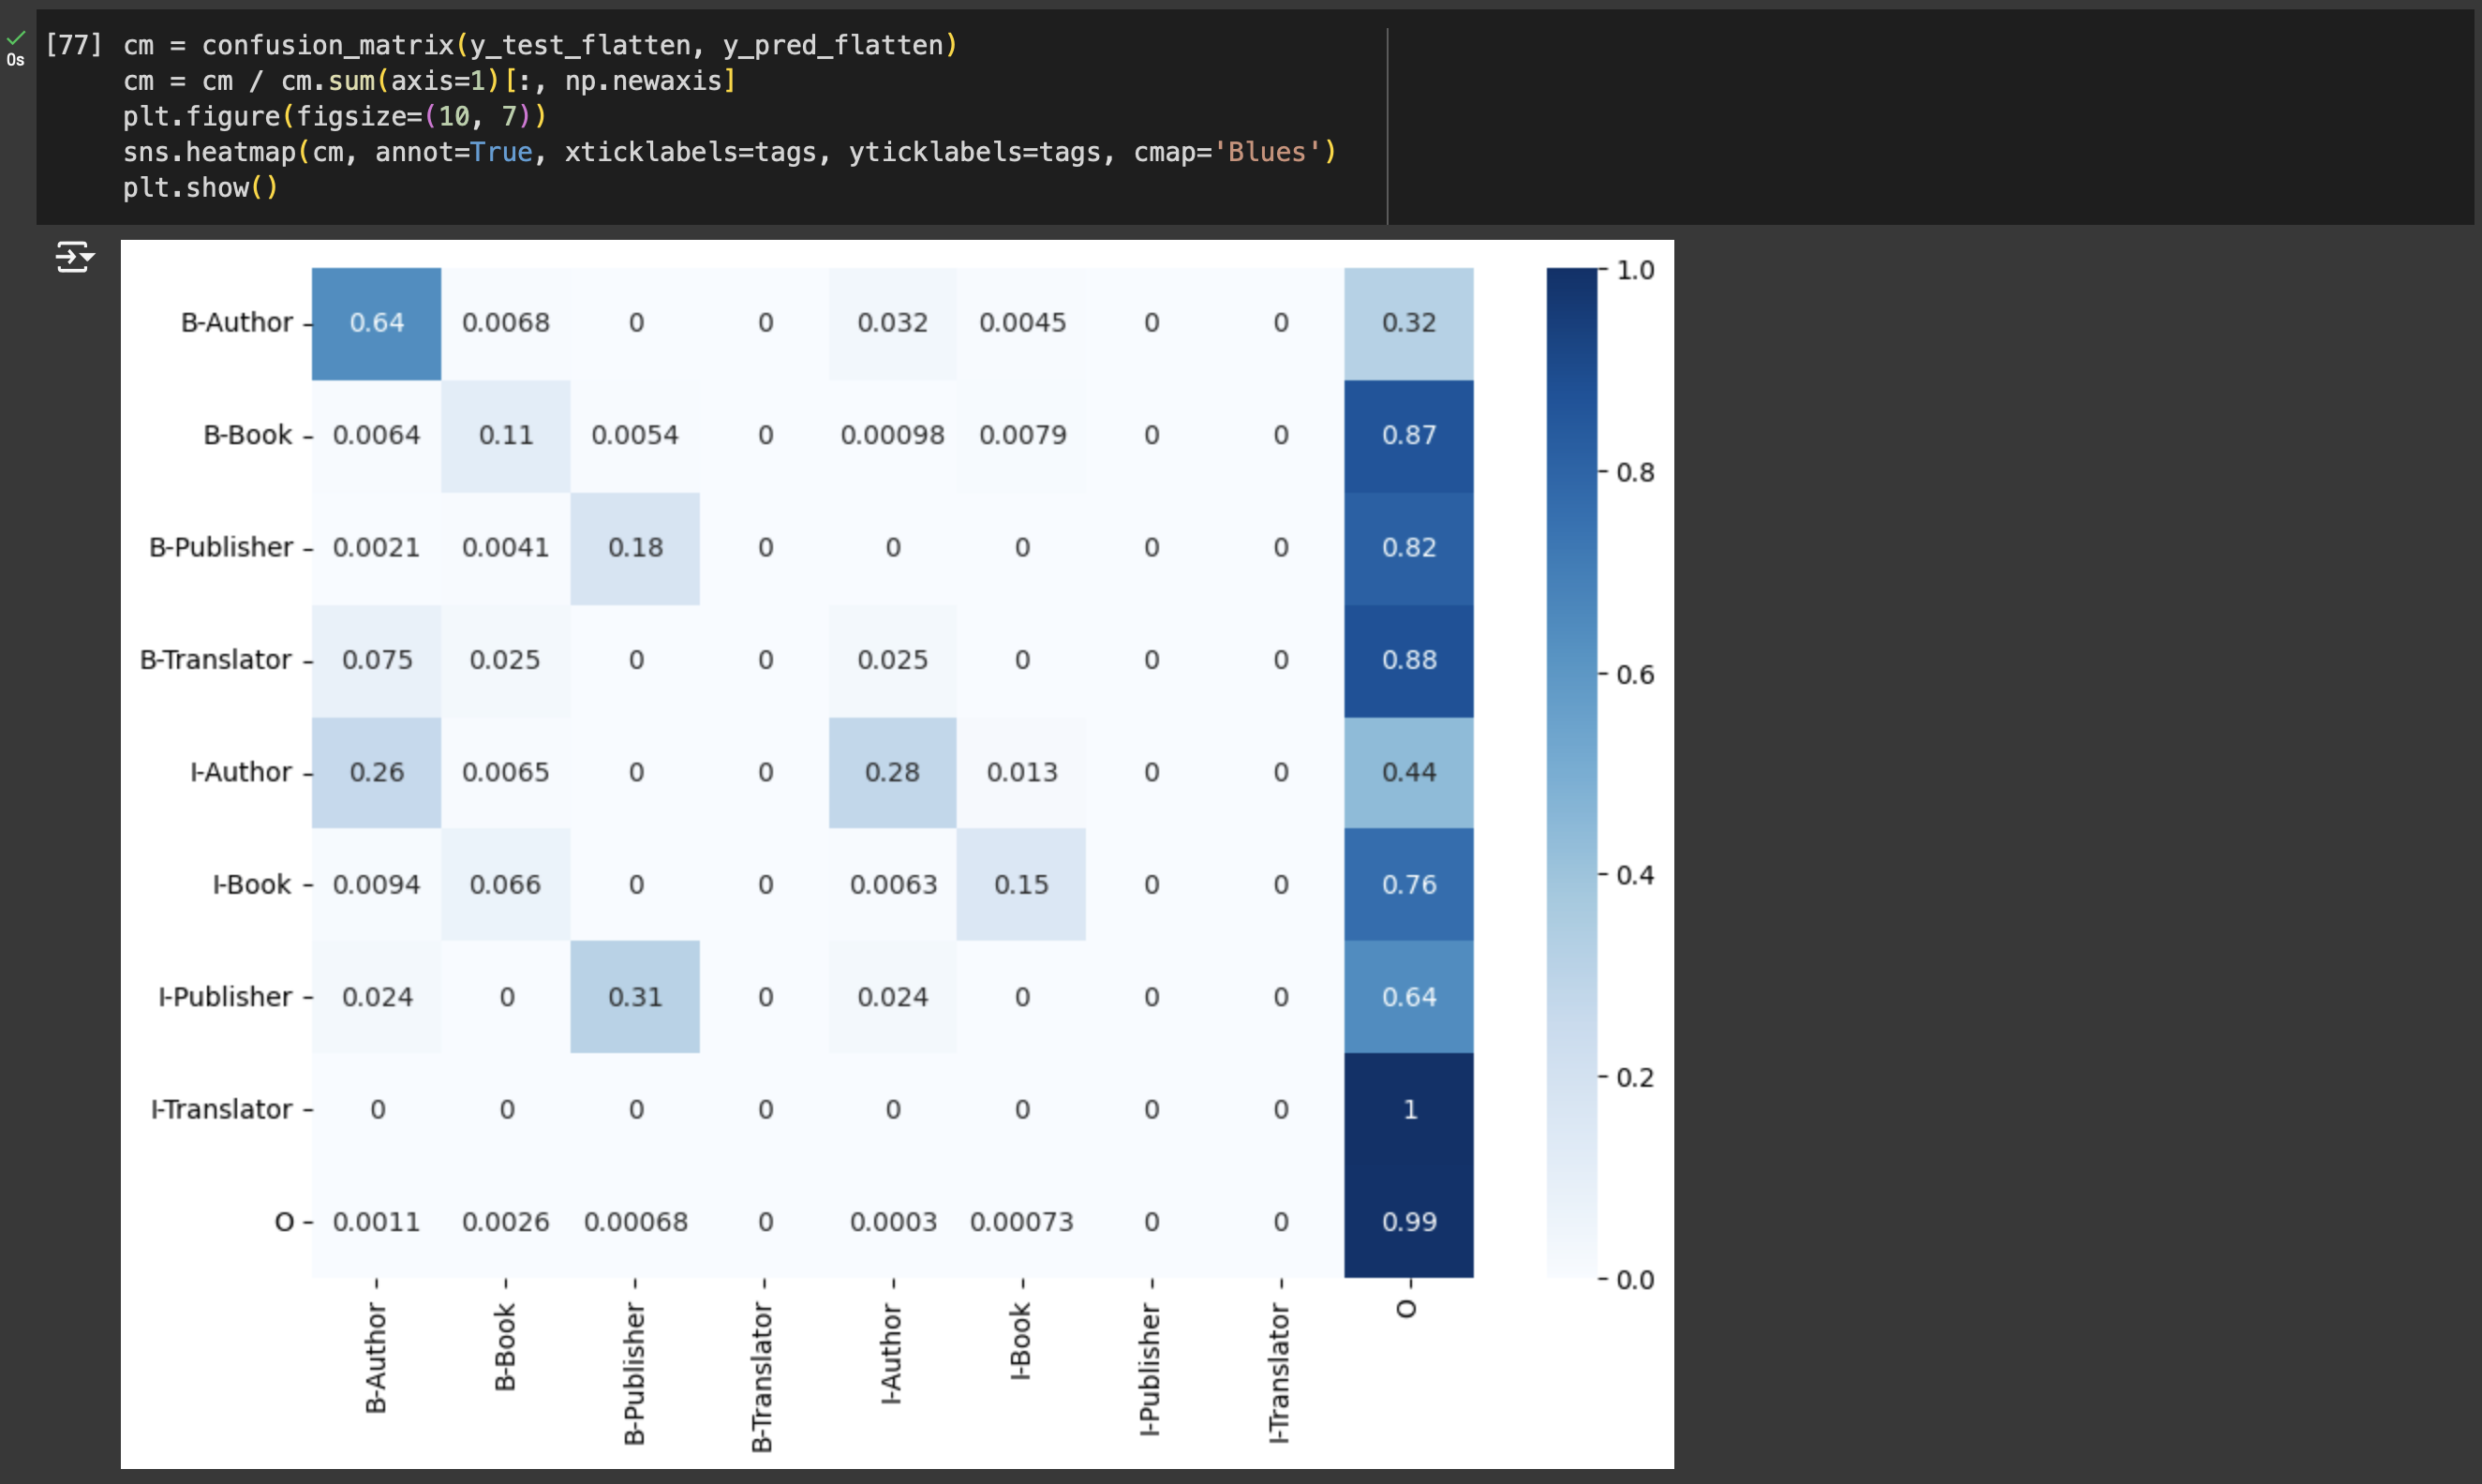
\includegraphics[width=0.5\textwidth]{img/1/11.png}
\end{figure}

\begin{figure}[h!]
    \caption{Metrics}
    \centering
    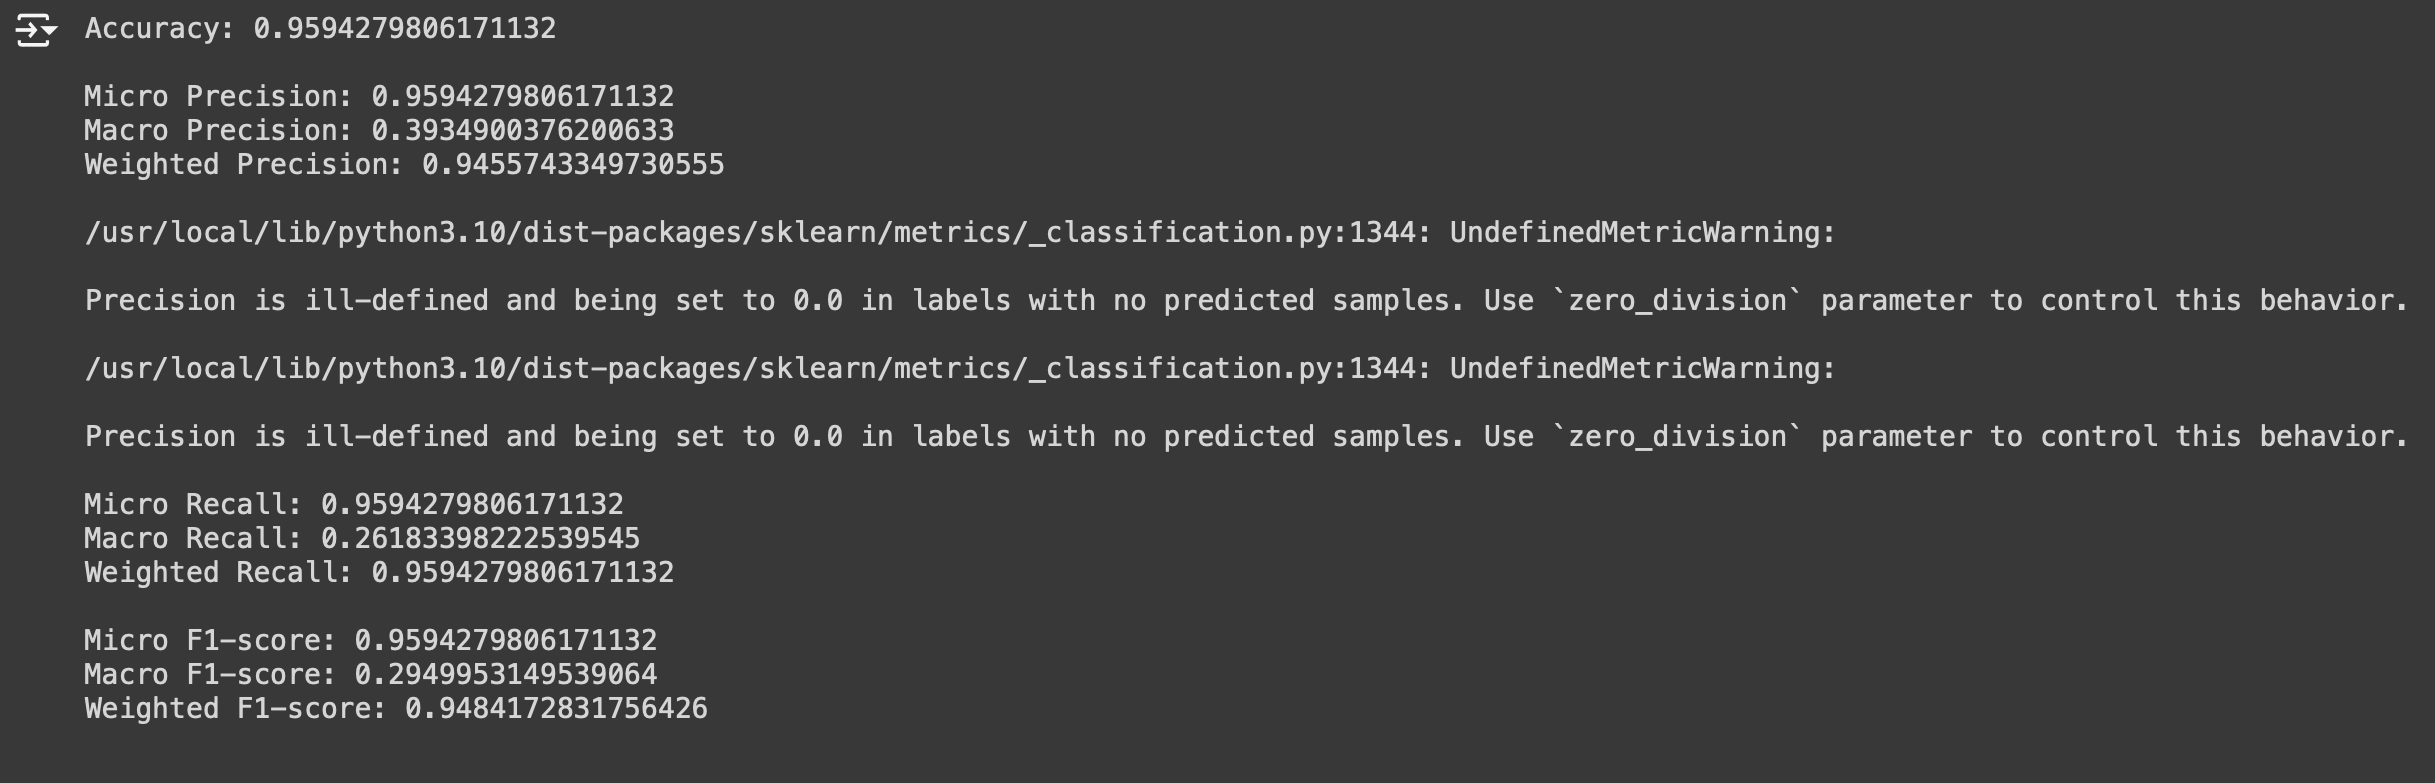
\includegraphics[width=0.5\textwidth]{img/1/12.png}
\end{figure}


\section{Word Classifier -  Transfomer Model}

The first part is exactly similar to the previous section. The only difference is that BERT is used as a normalizer. So, we explain only the transformer model in this section.



\begin{solution}


\begin{lstlisting}
    from transformers import BertConfig
    from transformers import TFBertForTokenClassification, InputFeatures
    import tensorflow as tf
    from livelossplot.tf_keras import PlotLossesCallback
    from sklearn.model_selection import train_test_split
    from sklearn.metrics import classification_report, accuracy_score, confusion_matrix, precision_score, recall_score, f1_score
    \end{lstlisting}
    
    First, the necessary libraries are imported. We use the Hugging Face Transformers library for BERT, TensorFlow for training, and various scikit-learn utilities for data handling and evaluation.
    
    \begin{lstlisting}
    tags = sorted(list(set([tag for label in labeled_data['label'] for tag in label])))
    tags_size = len(tags)
    tags_size, tags
    
    tag2idx = {tag: idx for idx, tag in enumerate(tags)}
    idx2tag = {idx: tag for tag, idx in tag2idx.items()}
    \end{lstlisting}
    
    The tags used for labeling are extracted and encoded into indices. The \texttt{tag2idx} and \texttt{idx2tag} dictionaries map tags to indices and vice versa.
    
    \begin{lstlisting}
    X_train, X_test, y_train, y_test = train_test_split(labeled_data['comment'], labeled_data['label'], test_size=0.2)
    X_val, X_test, y_val, y_test = train_test_split(X_test, y_test, test_size=0.5)
    
    train = pd.DataFrame({'comment': X_train, 'label': y_train})
    val = pd.DataFrame({'comment': X_val, 'label': y_val})
    test = pd.DataFrame({'comment': X_test, 'label': y_test})
    
    train = train[:64]
    val = val[:64]
    test = test[:64]
    
    train = train.reset_index(drop=True)
    val = val.reset_index(drop=True)
    test = test.reset_index(drop=True)
    \end{lstlisting}
    
    The labeled data is split into training, validation, and test sets using an 80-20 split, with the test set further split in half for validation. For demonstration purposes, only the first 64 rows of each dataset are used.
    
    \begin{lstlisting}
    def add_padding(data: pd.DataFrame, max_length: int):
        progress_bar = tqdm(range(len(data)))
        
        for i in progress_bar:
            data['comment'][i] = data['comment'][i][:max_length]
            data['label'][i] = data['label'][i][:max_length]
            
            if len(data['comment'][i]) < max_length:
                data['comment'][i] += ['[PAD]'] * (max_length - len(data['comment'][i]))
                data['label'][i] += ['O'] * (max_length - len(data['label'][i]))
                
        return data
    
    max_length = 128
    
    train = add_padding(train, max_length)
    val = add_padding(val, max_length)
    test = add_padding(test, max_length)
    \end{lstlisting}
    
    The \texttt{add\_padding} function ensures all comments and labels in the data are padded to a fixed length (\texttt{max\_length}). Padding is necessary for BERT to handle inputs of consistent length.
    
    \begin{lstlisting}
    ## Convert to GLUE Format
    
    class InputExample:
        def __init__(self, guid, text_a, text_b=None, label=None):
            self.guid = guid
            self.text_a = text_a
            self.text_b = text_b
            self.label = label
    \end{lstlisting}
    
    The \texttt{InputExample} class is defined to structure each data example with a unique ID, the text, and the label.
    
    \begin{lstlisting}
    def convert_data_to_examples(data: pd.DataFrame):
        examples = []
        
        for i in range(len(data)):
            guid = i
            text_a = data['comment'][i]
            label = data['label'][i]
            examples.append(InputExample(guid=guid, text_a=text_a, label=label))
            
        return examples
    
    
    def convert_examples_to_features(examples, tokenizer, max_length, task=None):
        features = []
        
        for example in examples:
            input_dict = tokenizer.encode_plus(
                example.text_a,
                add_special_tokens=True,
                max_length=max_length,
                return_token_type_ids=True,
                return_attention_mask=True,
                padding='max_length',
                truncation=True
            )
            
            input_ids = input_dict['input_ids']
            attention_mask = input_dict['attention_mask']
            token_type_ids = input_dict['token_type_ids']
            
            label = example.label
            
            if task is not None:
                label = [tag2idx[tag] for tag in label]
            
            features.append(
                InputFeatures(
                    input_ids=input_ids,
                    attention_mask=attention_mask,
                    token_type_ids=token_type_ids,
                    label=label
                )
            )
            
        return features
    
    
    def convert_data_to_features(data: pd.DataFrame, tokenizer, max_length, task=None):
        examples = convert_data_to_examples(data)
        return convert_examples_to_features(examples, tokenizer, max_length, task)
    \end{lstlisting}
    
    Functions are provided to convert data into examples and then into features suitable for BERT. These functions tokenize the text, add special tokens, and ensure padding and truncation to the maximum length.
    
    \begin{lstlisting}
    def convert_data_to_tf_dataset(data: pd.DataFrame, tokenizer, max_length, task=None):
        features = convert_data_to_features(data, tokenizer, max_length, task)
        
        all_input_ids = []
        all_attention_masks = []
        all_token_type_ids = []
        all_labels = []
        
        for feature in features:
            all_input_ids.append(feature.input_ids)
            all_attention_masks.append(feature.attention_mask)
            all_token_type_ids.append(feature.token_type_ids)
            all_labels.append(feature.label)
            
        return (
            tf.data.Dataset.from_tensor_slices((
                {
                    'input_ids': all_input_ids,
                    'attention_mask': all_attention_masks,
                    'token_type_ids': all_token_type_ids
                },
                all_labels
            ))
        )
    \end{lstlisting}
    
    The \texttt{convert\_data\_to\_tf\_dataset} function converts the features into a TensorFlow dataset suitable for training.
    
    \begin{lstlisting}
    max_length = 128
    task = 'ner'
    
    train_dataset = convert_data_to_tf_dataset(train, tokenizer, max_length, task=task)
    val_dataset = convert_data_to_tf_dataset(val, tokenizer, max_length, task=task)
    test_dataset = convert_data_to_tf_dataset(test, tokenizer, max_length, task=task)
    
    train_dataset = train_dataset.shuffle(100).batch(32).repeat(2)
    val_dataset = val_dataset.batch(64)
    test_dataset = test_dataset.batch(64)
    
    train_dataset.element_spec, val_dataset.element_spec, test_dataset.element_spec
    \end{lstlisting}
    
    The datasets for training, validation, and testing are prepared, shuffled, and batched appropriately.
    
    \begin{lstlisting}
    config = BertConfig.from_pretrained(MODEL_NAME_OR_PATH, num_labels=tags_size, id2label=idx2tag, label2id=tag2idx)
    
    model = TFBertForTokenClassification.from_pretrained(MODEL_NAME_OR_PATH, config=config)
    model.summary()
    
    multi_label_loss = tf.keras.losses.SparseCategoricalCrossentropy(from_logits=True)
    model.compile(optimizer='adam', loss=multi_label_loss, metrics=['accuracy'])
    
    plot_losses = PlotLossesCallback()
    
    model.fit(train_dataset, epochs=1, validation_data=val_dataset, callbacks=[plot_losses])
    \end{lstlisting}
    
    The BERT model is configured and initialized for token classification. The model is compiled with a loss function and accuracy metric, and training is initiated with the \texttt{fit} method, including a callback for plotting the training losses.
    
\end{solution}

\newpage
\subsection*{Results and Imporatnt Notes}

We must note that we tried to use Hazm's Informal Normalizer but it was very slow. So, صe customized the Hazm Informal Normalizer. It returns a 3D array in which the third dimension is a candidate for the formal word. We picked the first candidate directly by customizing the Hazm library. Now, it returns a 2D array, and its performance has improved.

For labeling, we iterate over comments and check if the word is in, as an example, in the book name or not. If it was in the book name’s list, we appended the index of the word in the book name’s list to a list. So now we have a list of indexes. Then, we tried to find all consecutive ascending sequences in the list. Then we tag them by BIO, or if they are -1, we tag them by O.


Another important note is related to the distribution of tags. The "O" tag completely dominates other tags by count, and therefore, it impacts our results. You can see the distribution in the following figures.



\begin{figure}[h!]
    \caption{Percentage of O in Each Label List Histogram}
    \centering
    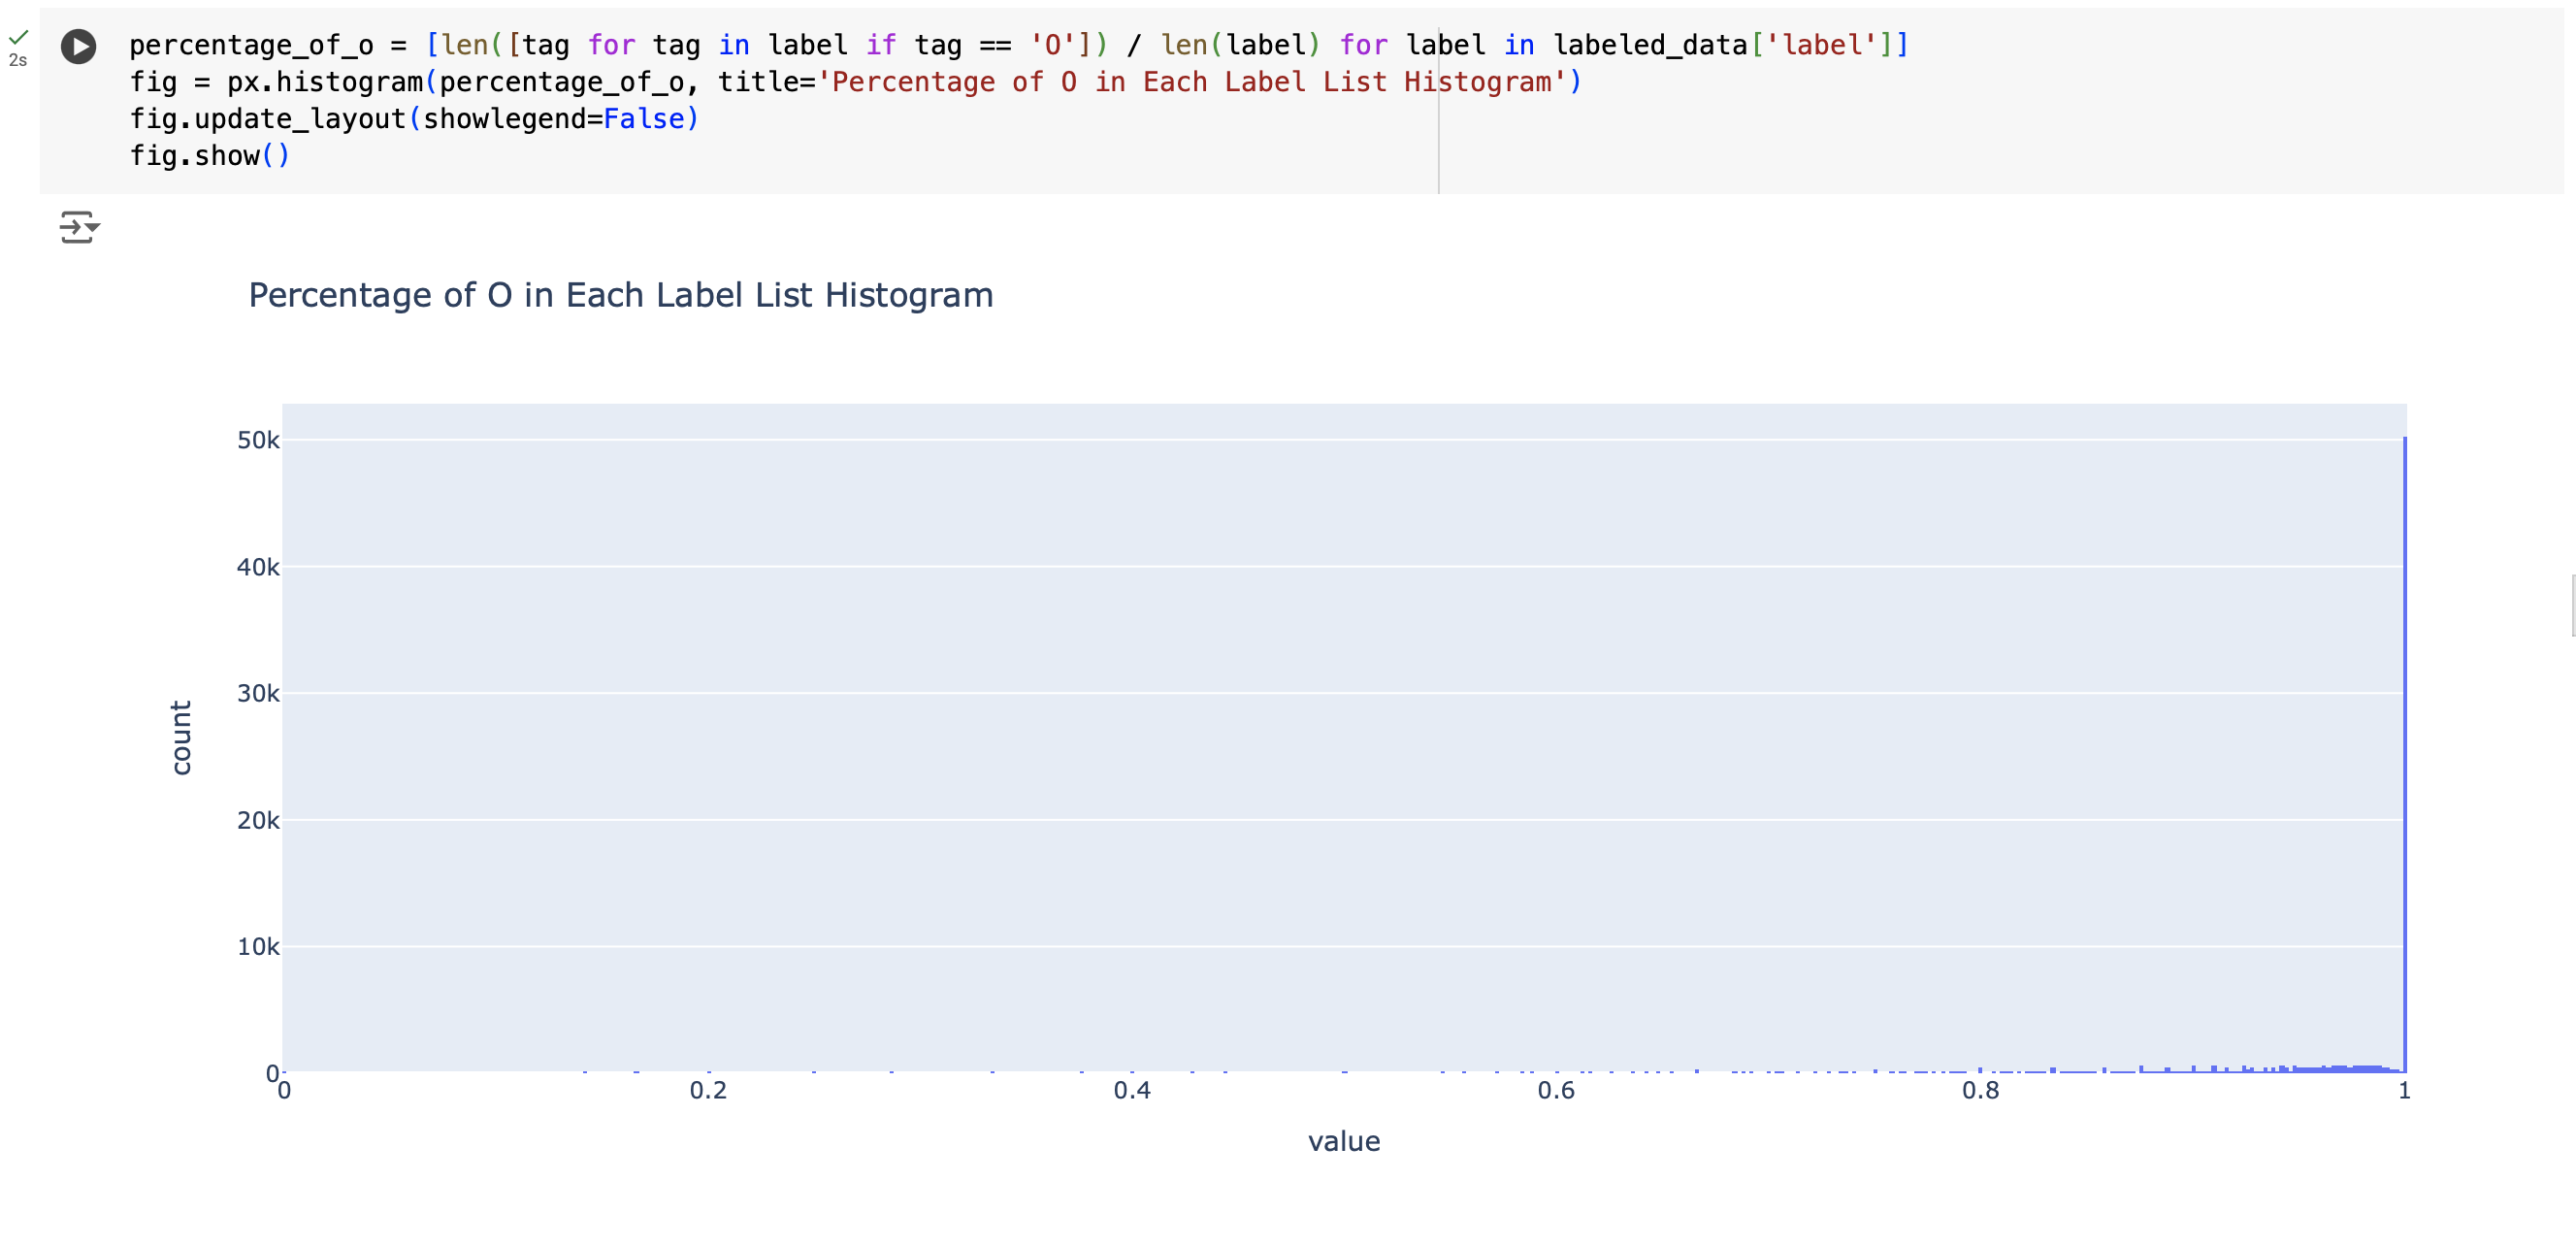
\includegraphics[width=0.5\textwidth]{img/2/1.png}
\end{figure}

\begin{figure}[h!]
    \caption{ Tag Distribution with O}
    \centering
    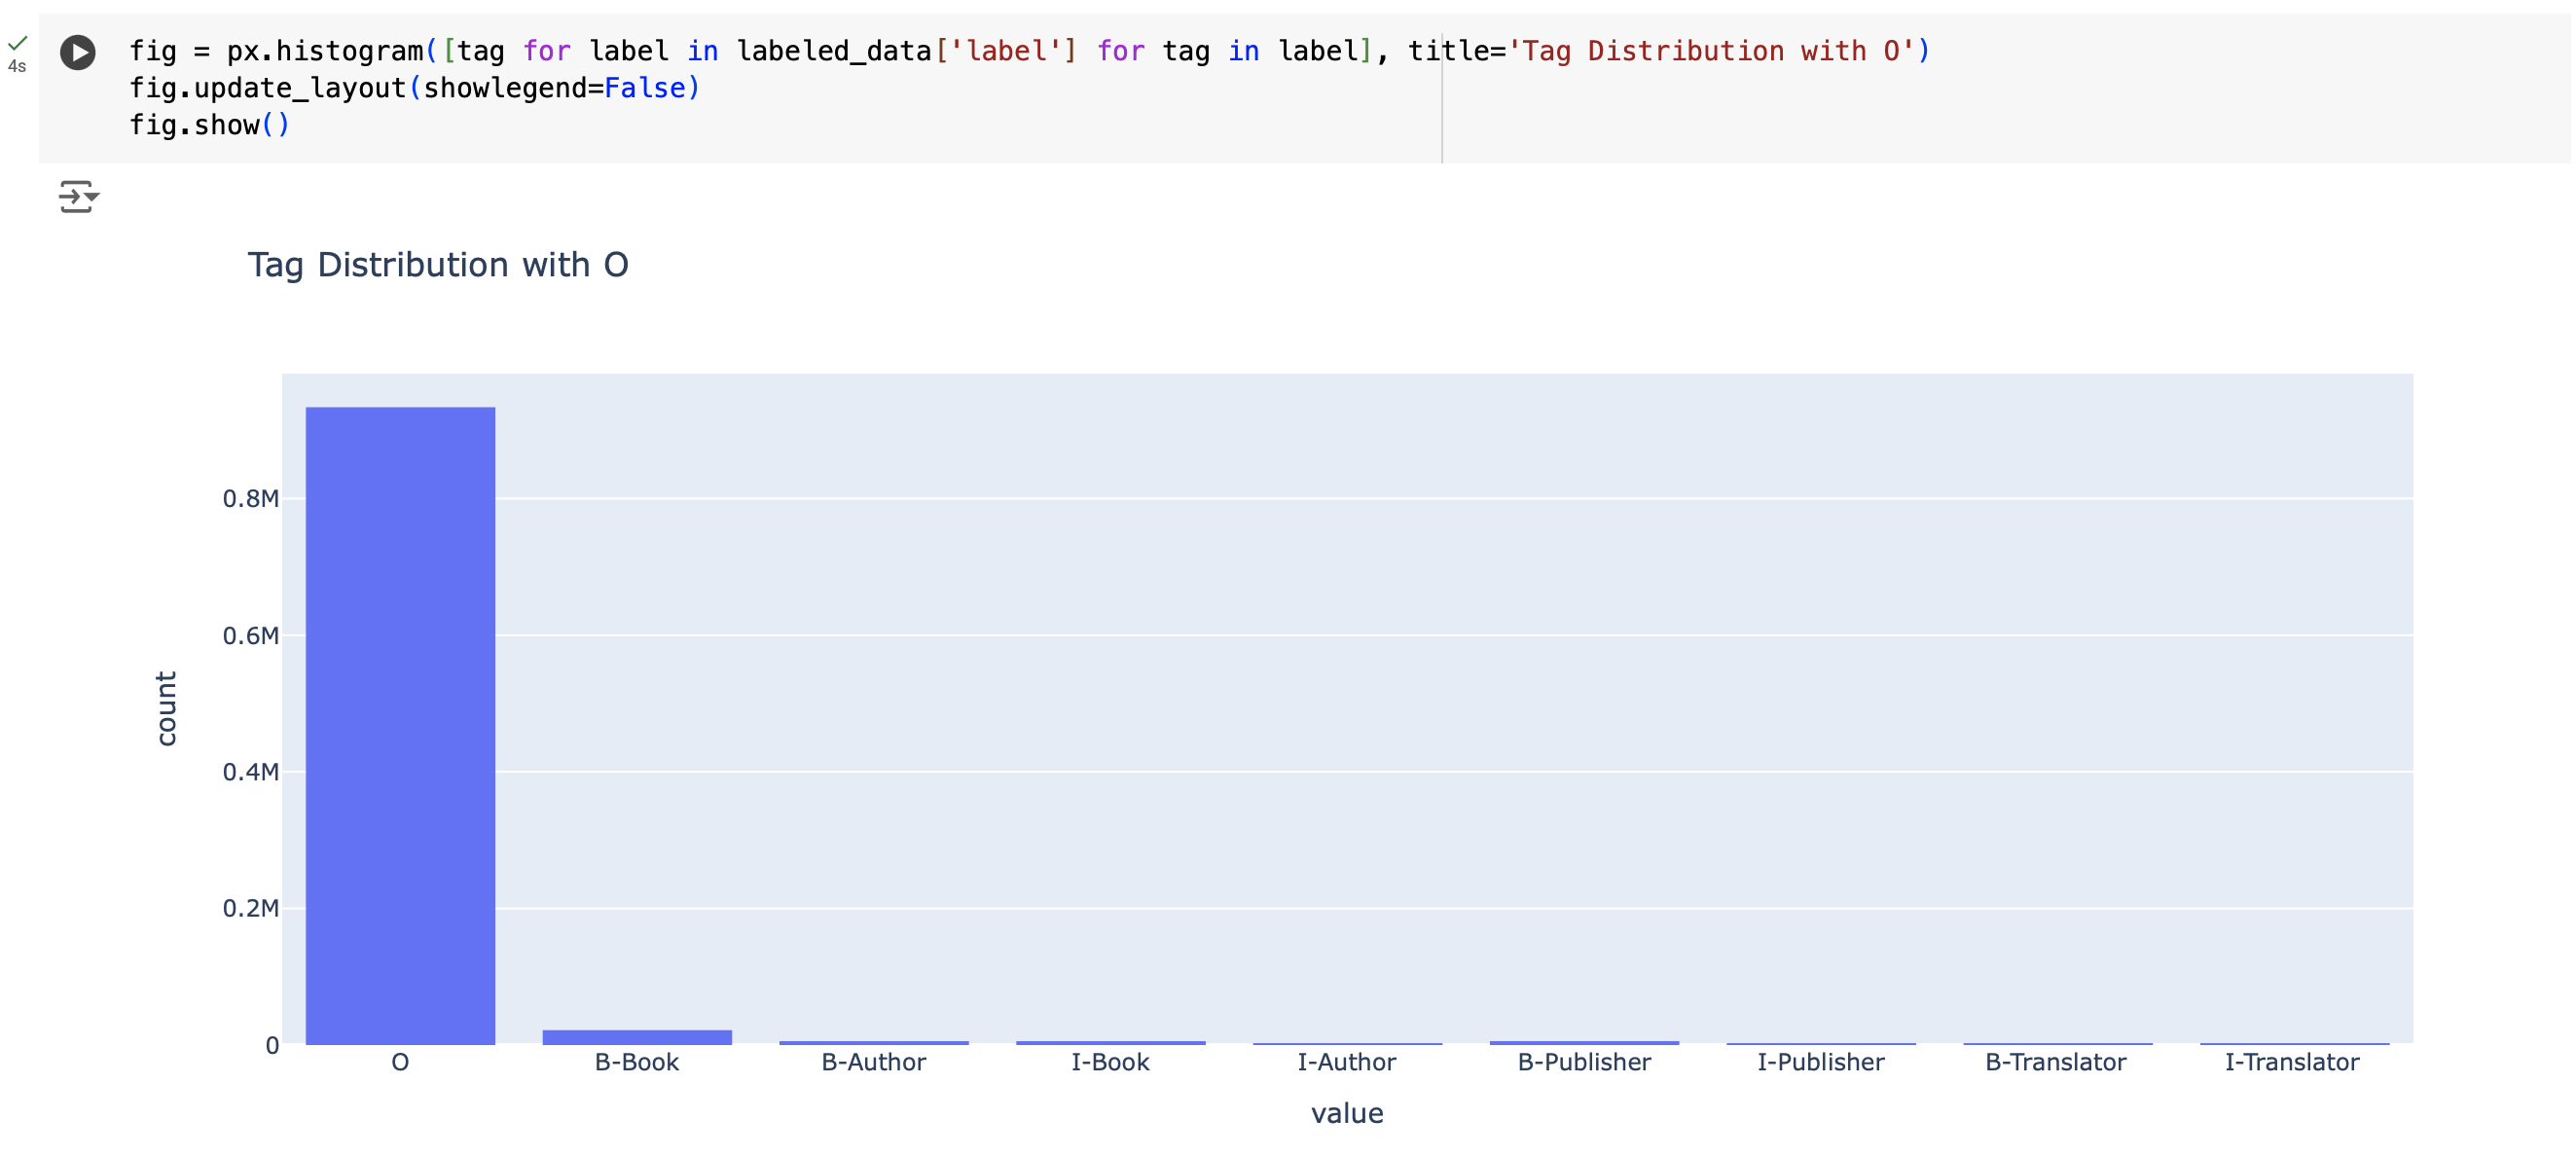
\includegraphics[width=0.5\textwidth]{img/2/2.png}
\end{figure}


\begin{figure}[h!]
    \caption{Tag distribution without O}
    \centering
    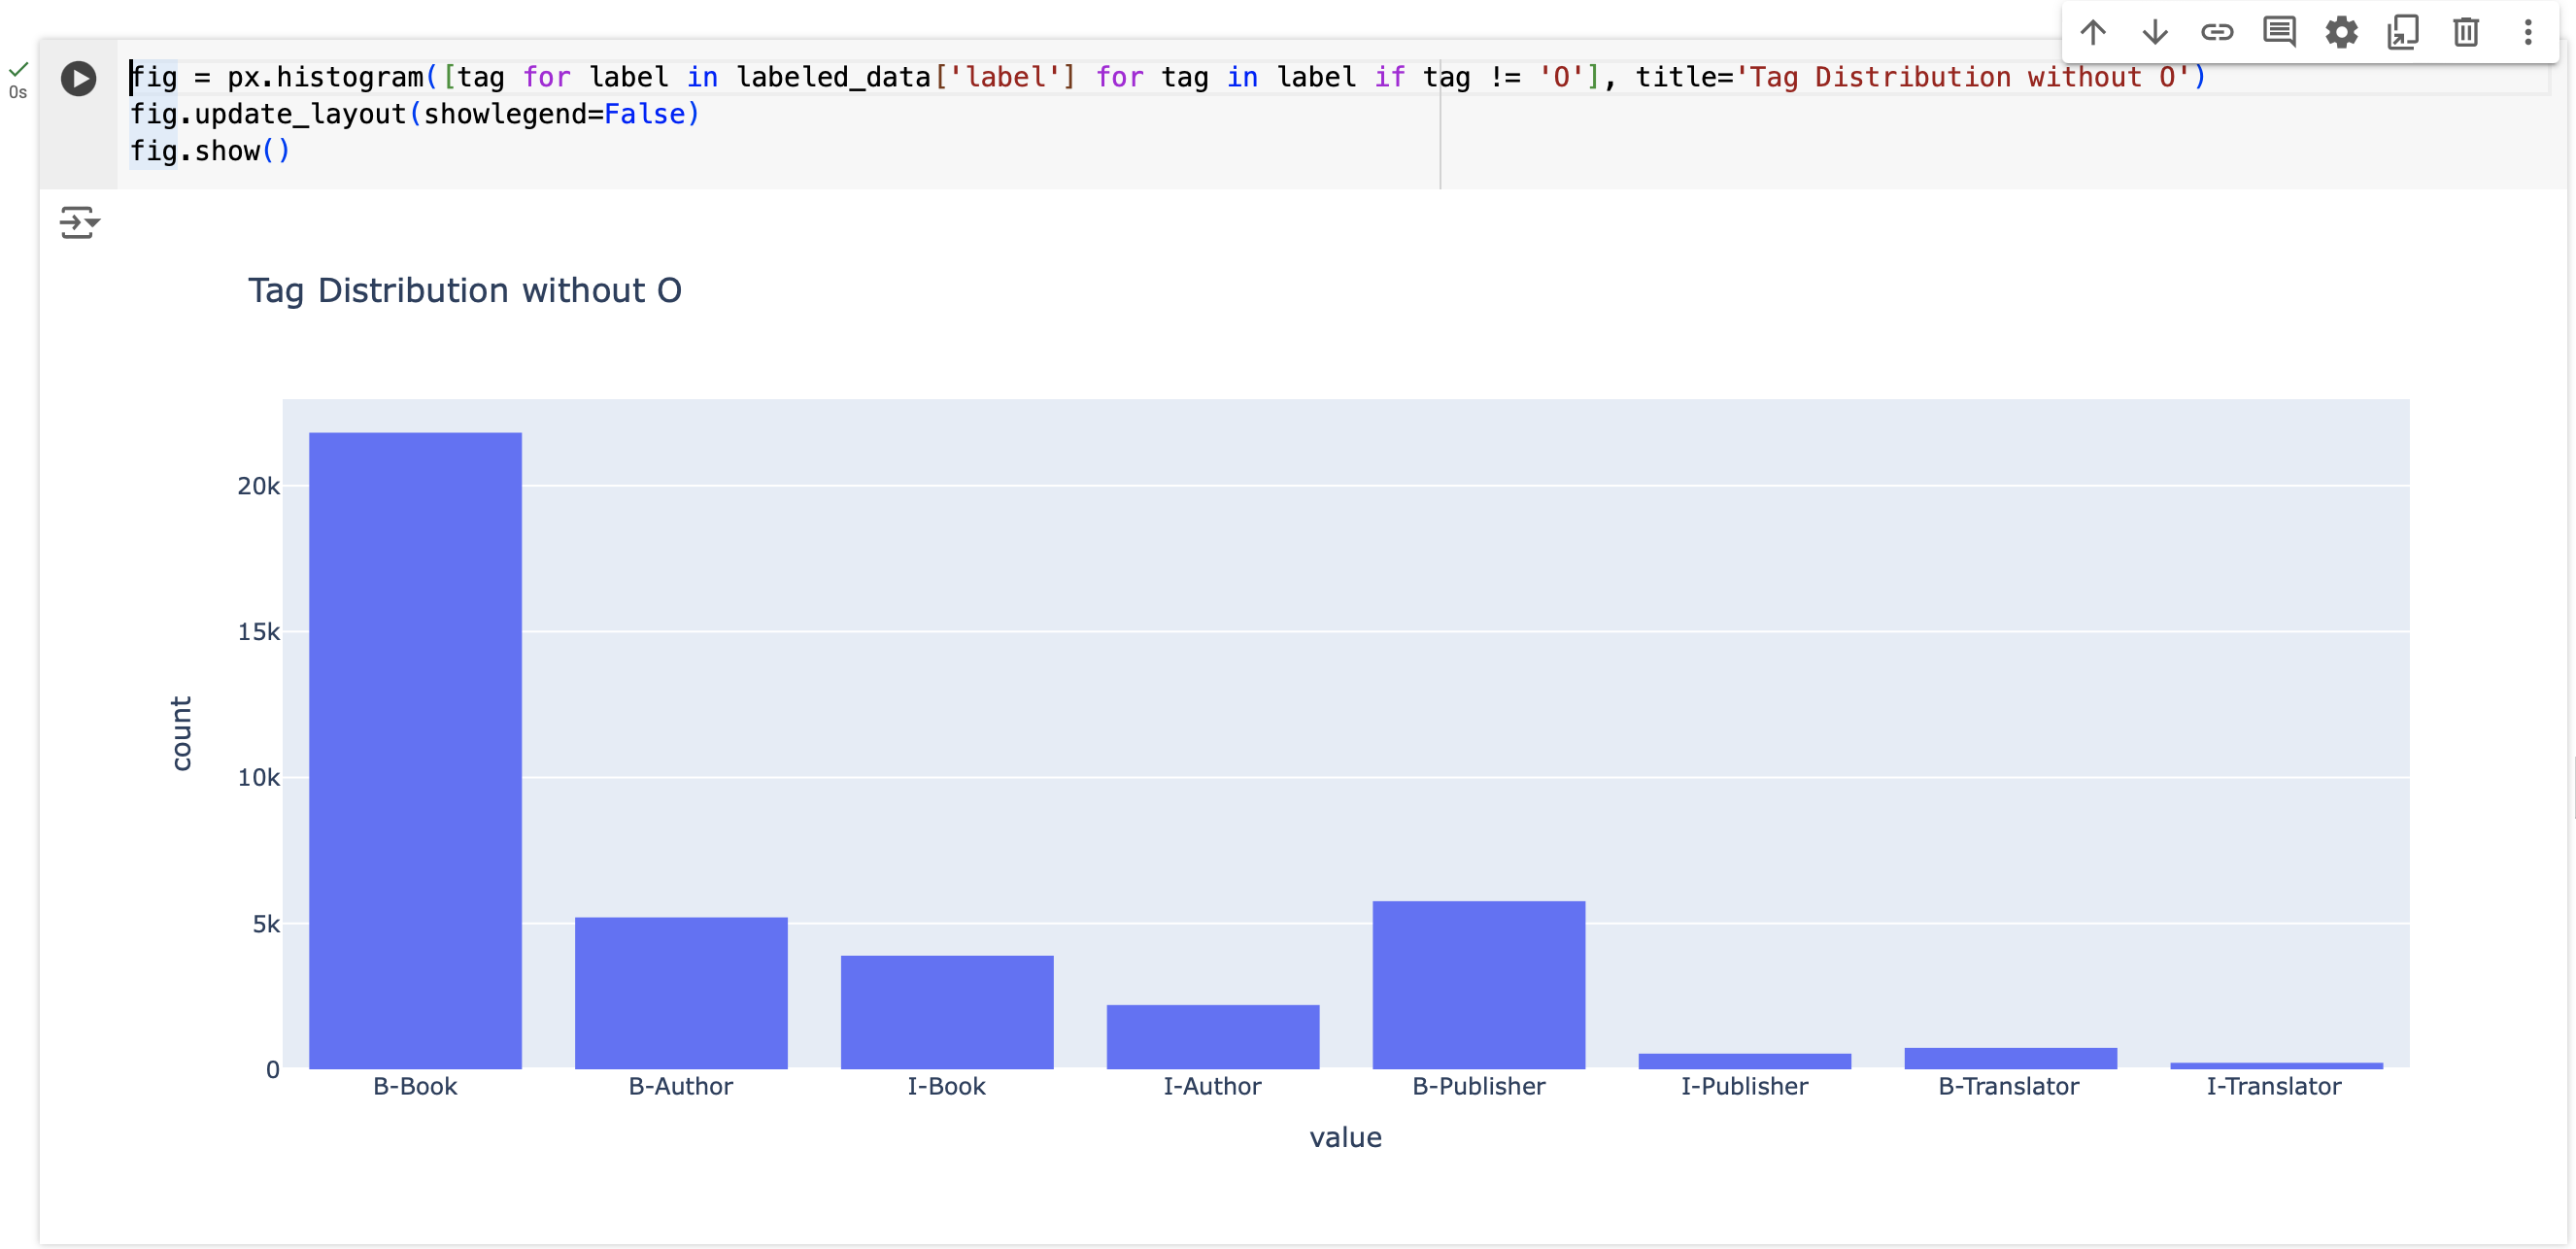
\includegraphics[width=0.5\textwidth]{img/2/3.png}
\end{figure}

\begin{figure}[h!]
    \caption{Transfomer Model}
    \centering
    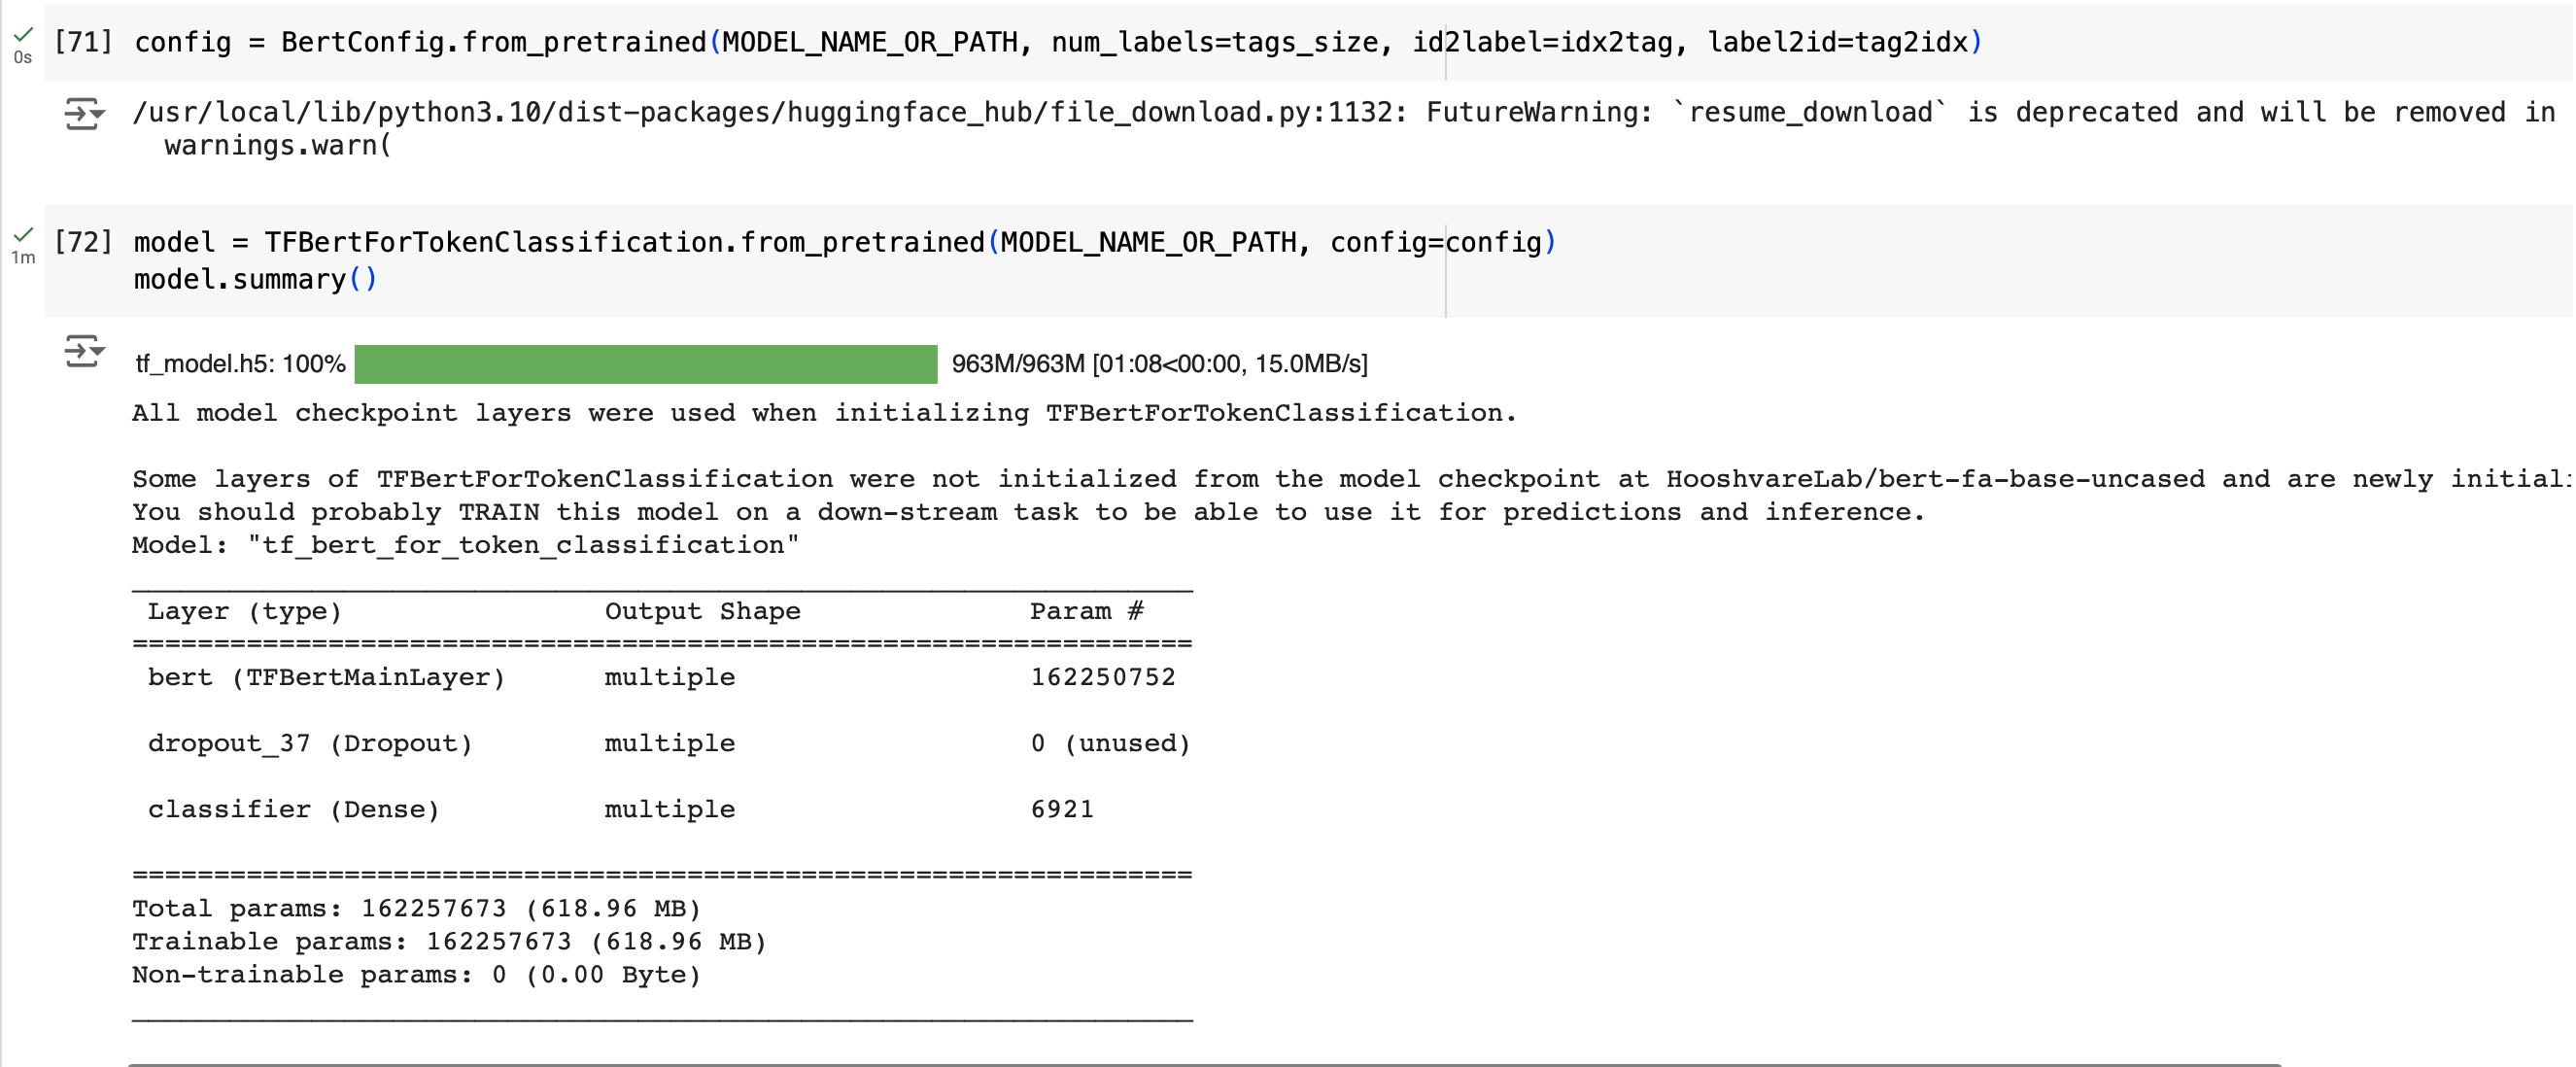
\includegraphics[width=0.5\textwidth]{img/2/4.png}
\end{figure}

\begin{figure}[h!]
    \caption{ Accuracy and Loss During Training}
    \centering
    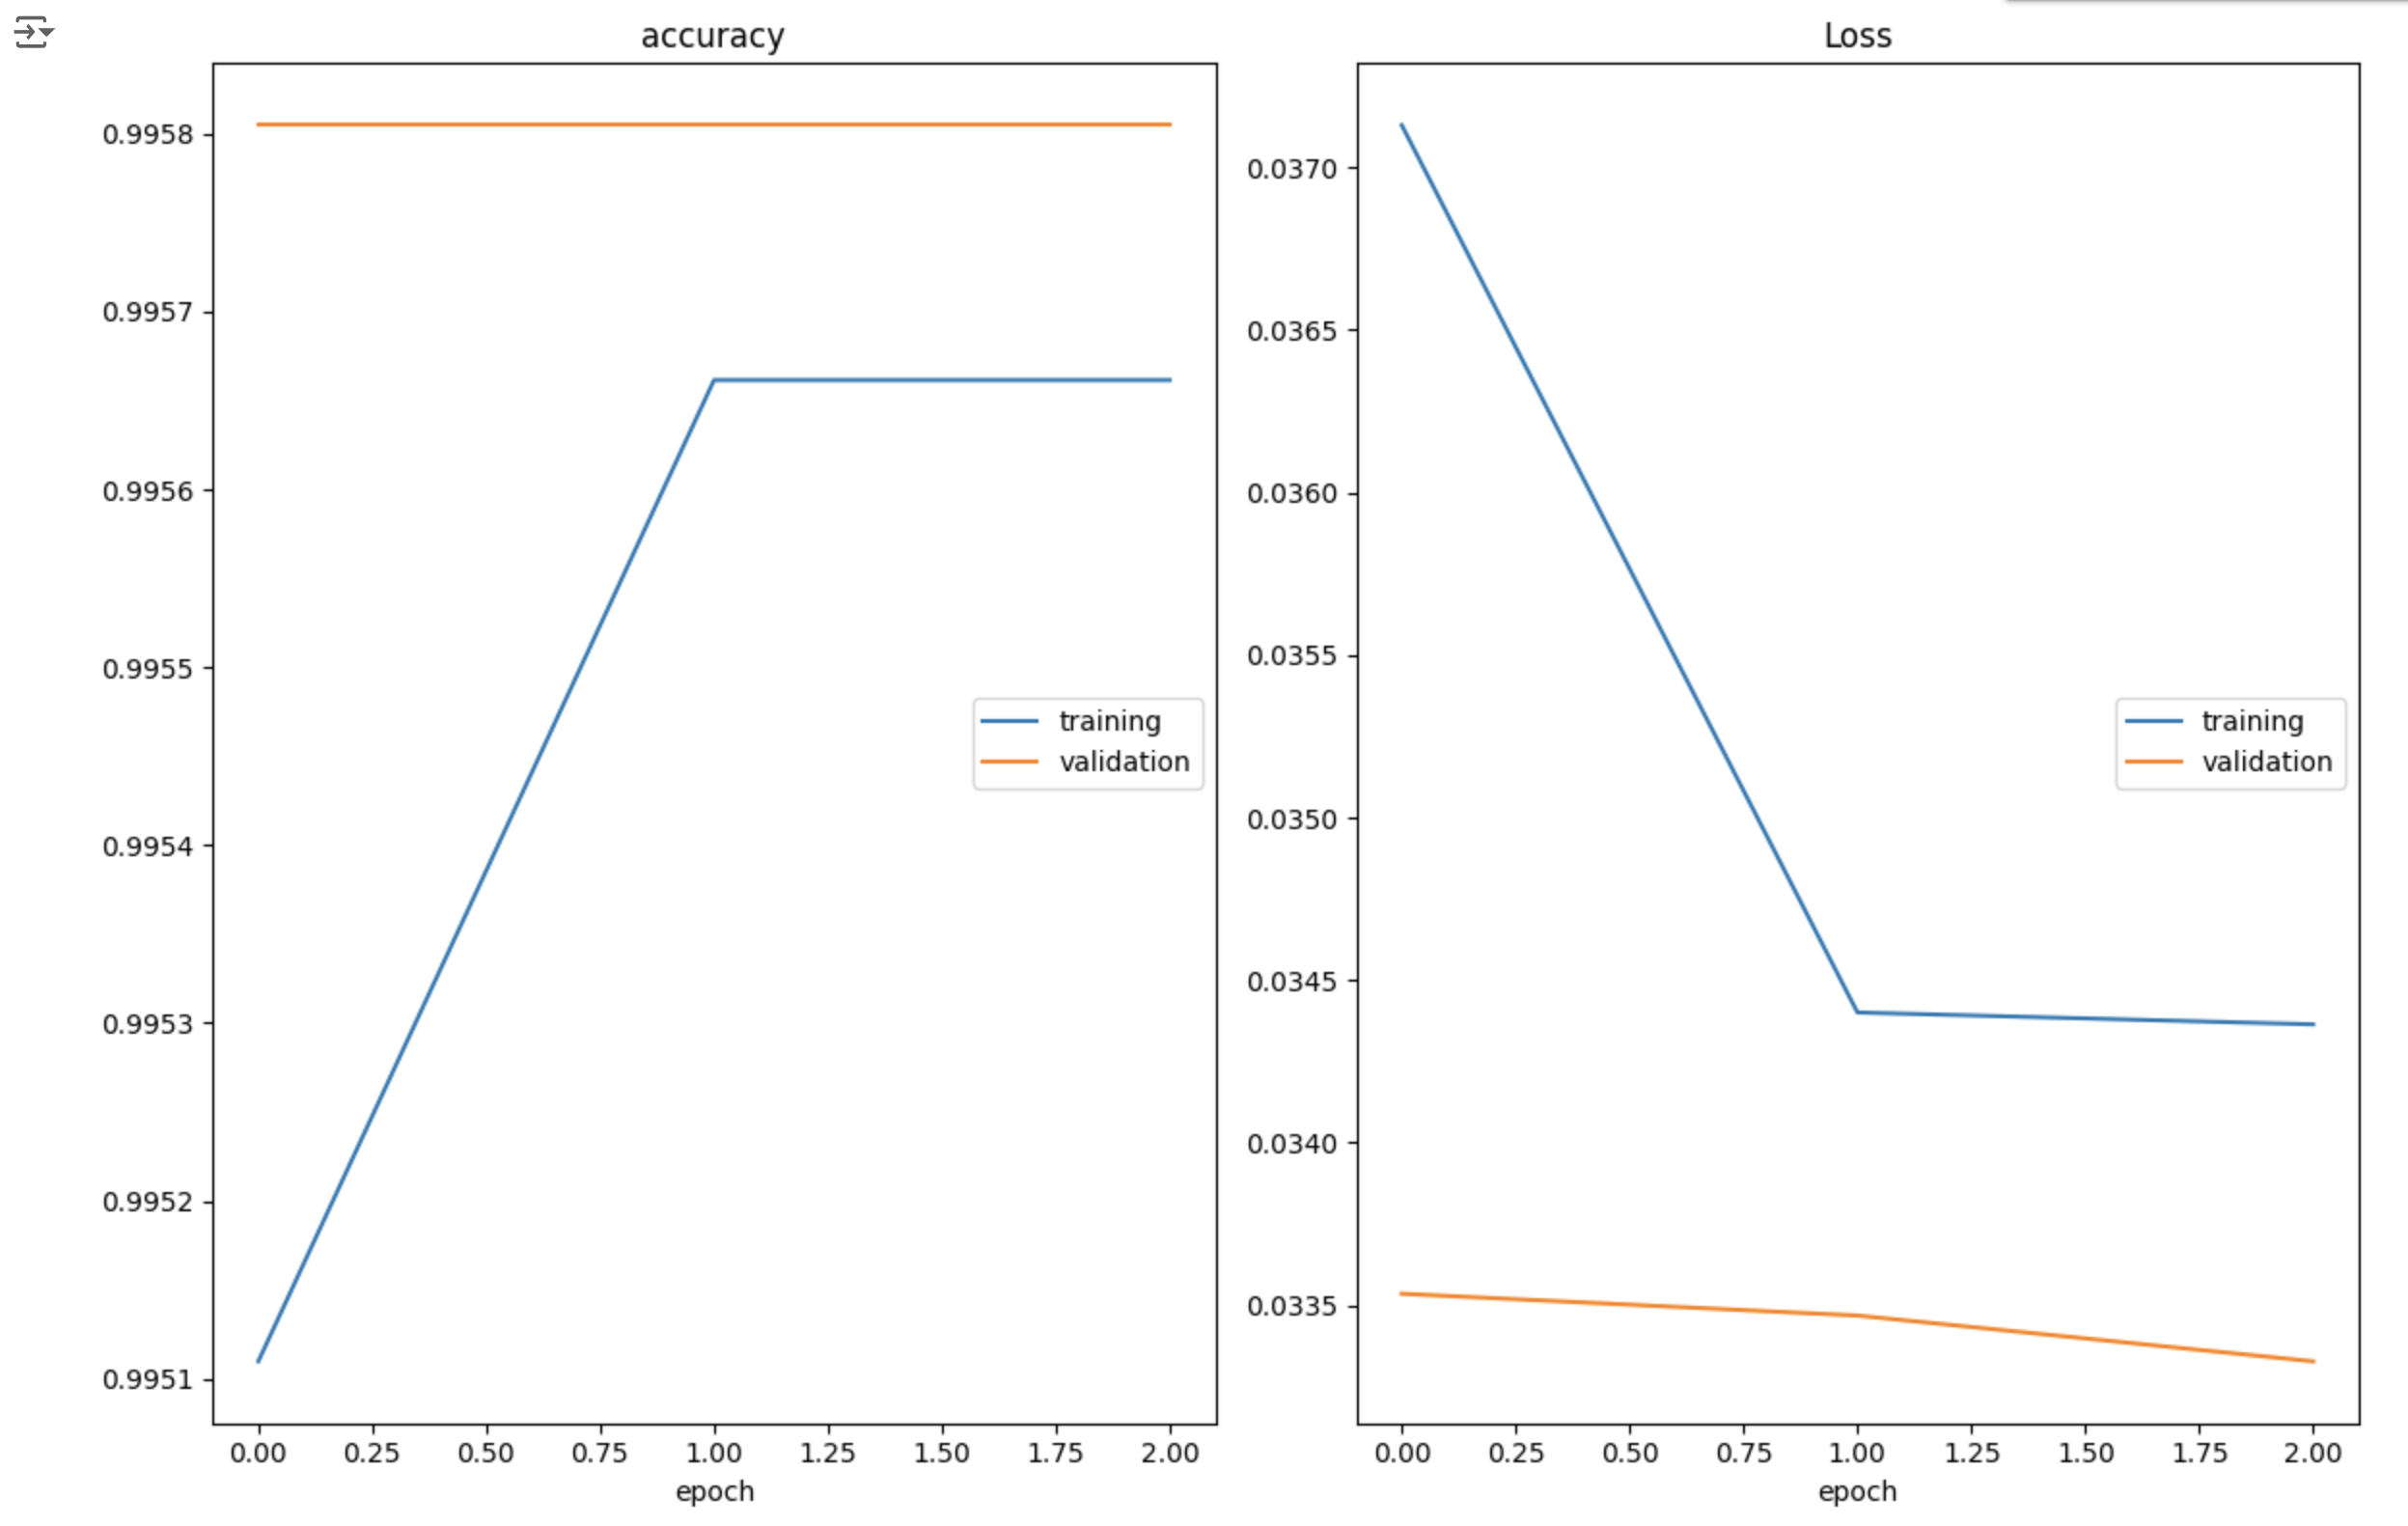
\includegraphics[width=0.5\textwidth]{img/2/5.png}
\end{figure}

\begin{figure}[h!]
    \caption{Some Evaluations}
    \centering
    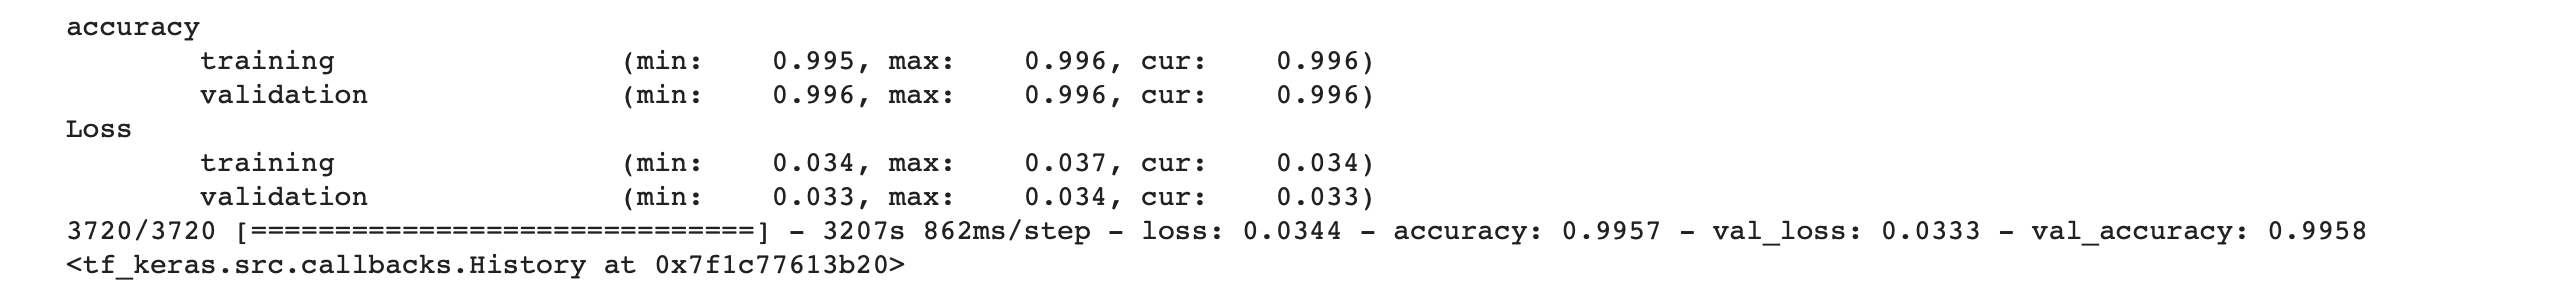
\includegraphics[width=0.5\textwidth]{img/2/6.png}
\end{figure}

\begin{figure}[h!]
    \caption{Classification Report}
    \centering
    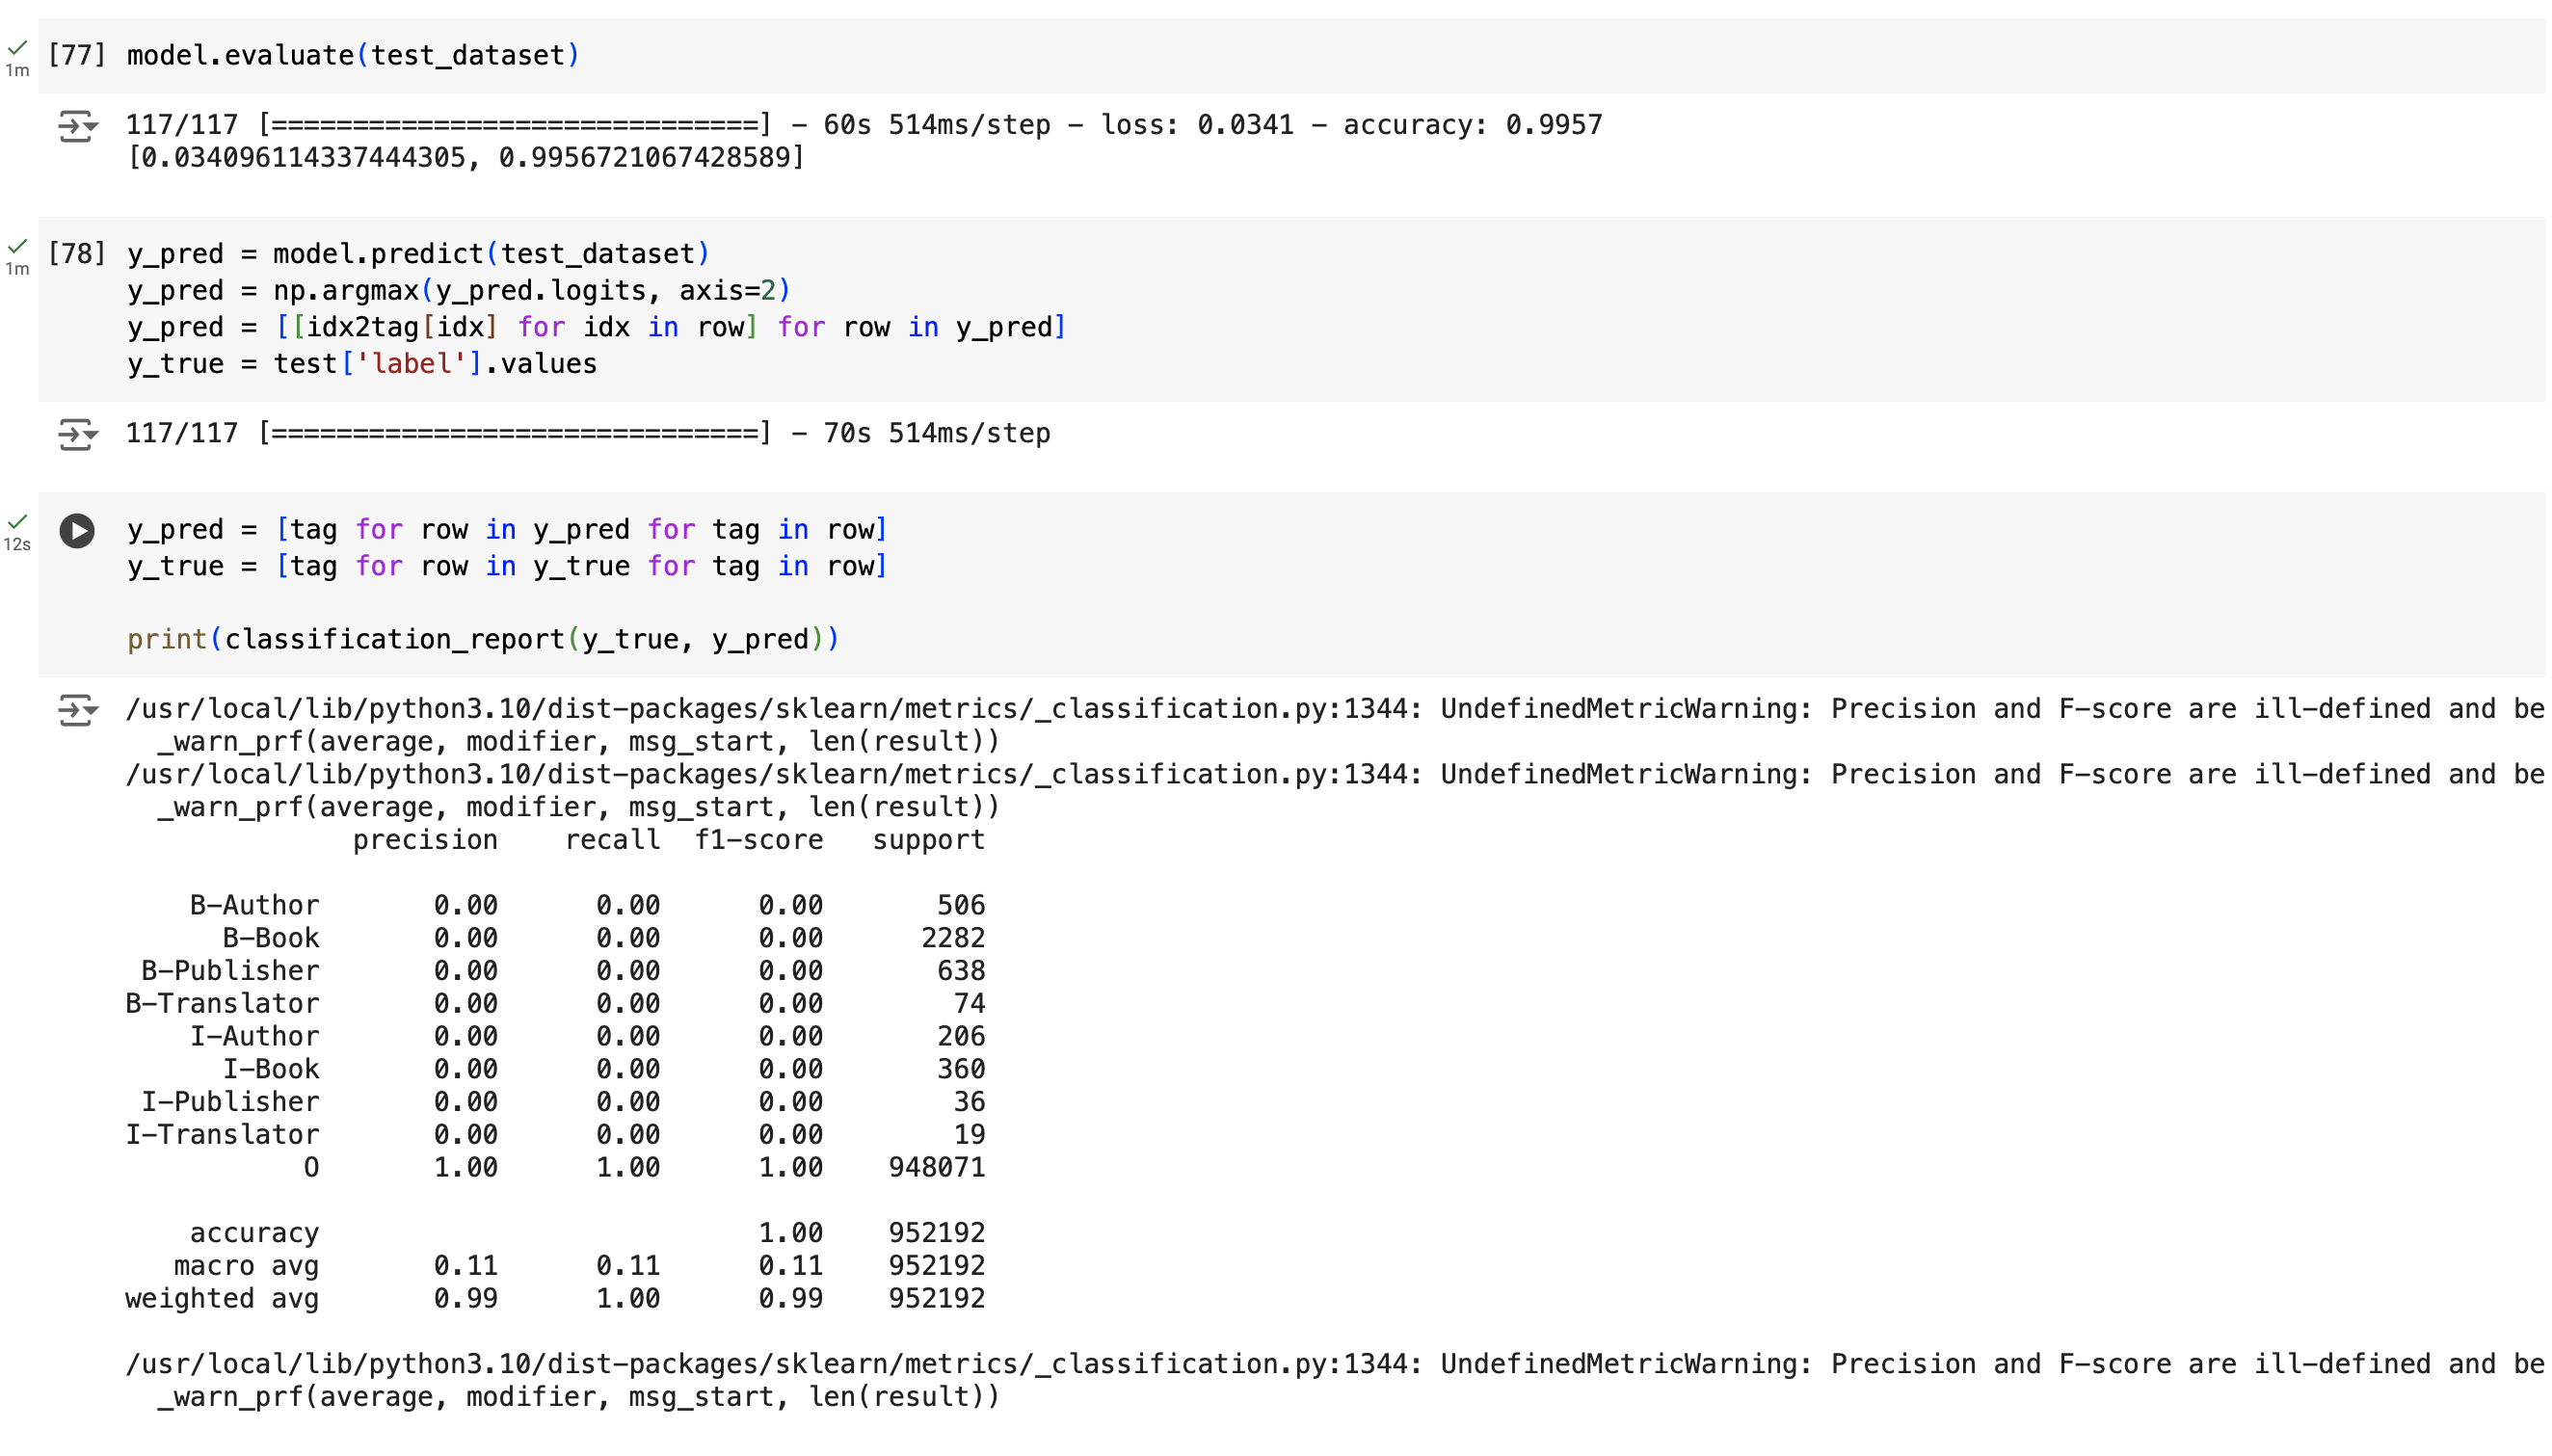
\includegraphics[width=0.5\textwidth]{img/2/7.png}
\end{figure}
\newpage
\begin{figure}[h!]
    \caption{Confusion matrix}
    \centering
    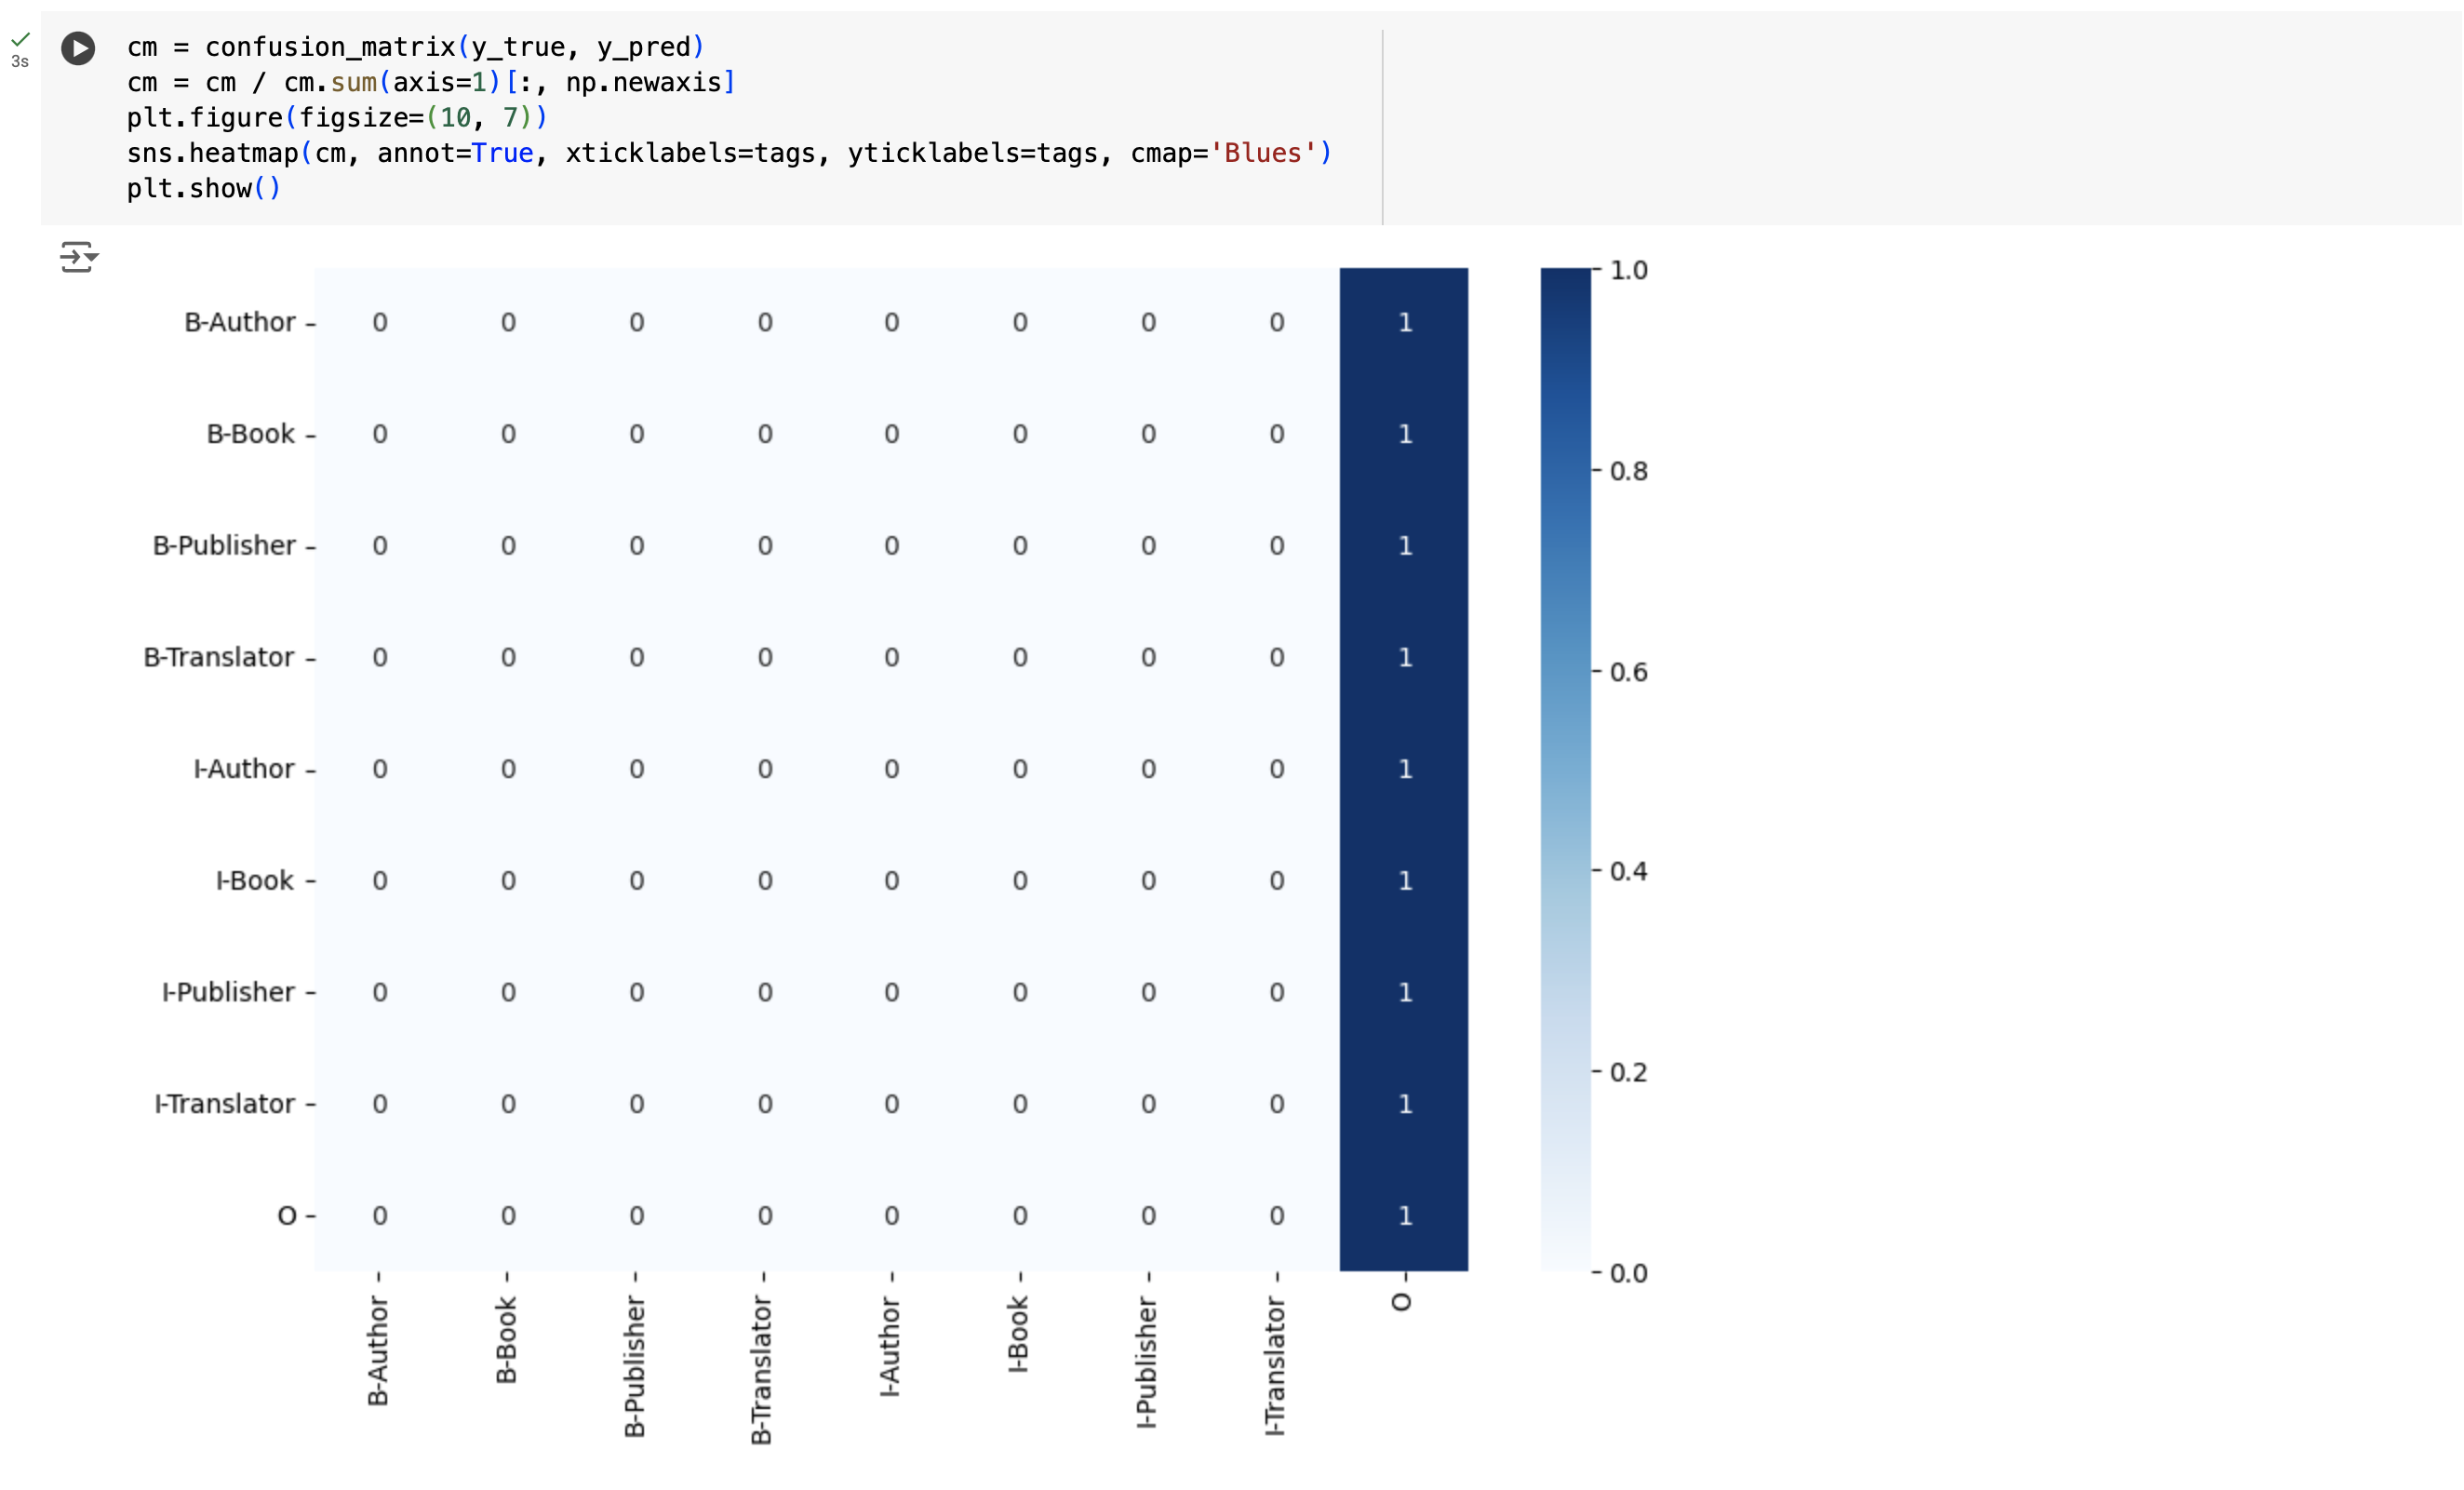
\includegraphics[width=0.5\textwidth]{img/2/8.png}
\end{figure}







\end{document}












